%%%%%%%%%%%%%%%%%%%%%%%%%%%%%%%%%%%%%%%%%%%%%%%%%%%%%%%%%%%%%%%%%
%  _____   ____  _____                                          %
% |_   _| /  __||  __ \    Institute of Computitional Physics   %
%   | |  |  /   | |__) |   Zuercher Hochschule Winterthur       %
%   | |  | (    |  ___/    (University of Applied Sciences)     %
%  _| |_ |  \__ | |        8401 Winterthur, Switzerland         %
% |_____| \____||_|                                             %
%%%%%%%%%%%%%%%%%%%%%%%%%%%%%%%%%%%%%%%%%%%%%%%%%%%%%%%%%%%%%%%%%
%
% Project     : LaTeX doc Vorlage für Windows ProTeXt mit TexMakerX
% Title       : 
% File        : header.tex Rev. 00
% Date        : 23.4.12
% Author      : Remo Ritzmann
% Feedback bitte an Email: remo.ritzmann@pfunzle.ch
%
%%%%%%%%%%%%%%%%%%%%%%%%%%%%%%%%%%%%%%%%%%%%%%%%%%%%%%%%%%%%%%%%%

\documentclass[ oneside,openright,titlepage,numbers=noenddot,headinclude,%1headlines,% letterpaper a4paper
                BCOR=5mm,paper=a4,fontsize=11pt,%11pt,a4paper,%
                ngerman,american,%
                ]{scrreprt}

%***********************************************************************
% include some libs
%***********************************************************************
\usepackage[utf8]{inputenc}
\usepackage{listings}
\usepackage{color}
\usepackage{fancyhdr}
\usepackage{rotating}
\usepackage{titlesec}
\usepackage{mathptmx}
% \usepackage{helvet}
\usepackage[scaled]{uarial}
\renewcommand*\familydefault{\sfdefault} %% Only if the base font of the document is to be sans serif
\usepackage[T1]{fontenc}
\usepackage{ngerman}
\usepackage{textgreek}
\usepackage{textcomp}
\usepackage[squaren]{SIunits}
\usepackage{graphicx}
\usepackage{url}
\usepackage{geometry}
\usepackage[absolute]{textpos}
\usepackage{makeidx}
\usepackage{colortbl}
\usepackage{pdflscape}
\usepackage{pdfpages}
\usepackage{tabularx}
\usepackage{lmodern}
\usepackage{longtable}
\usepackage{array}
\usepackage{float}
\usepackage{scrhack}
\usepackage[plainpages=false]{hyperref}
\usepackage{wallpaper} %\ThisTileWallPaper{}
%\usepackage[super,square]{natbib} für BibTeX Literaturverzeichnis
\usepackage{enumitem}
\usepackage{subfig}
\usepackage[export]{adjustbox}
\usepackage{setspace}
\usepackage{amsmath} 
\usepackage{fancyvrb}
\usepackage{graphicx}
\usepackage{booktabs}

% Bibliography
\usepackage[
backend=bibtex,
style=alphabetic-verb,
citestyle=alphabetic-verb
]{biblatex}
\bibliography{./Citer}

\usepackage{calc}



%***********************************************************************
% various styles
%***********************************************************************	

%create index
\makeindex

%define pagestyle
\pagestyle{fancy}

%use sans-serif font 
%\renewcommand{\familydefault}{\sfdefault}

%define page margin
\geometry{a4paper, top=30mm, left=30mm, right=30mm, bottom=30mm,headsep=10mm,footskip=10mm}

%textpos parameter
\setlength{\TPHorizModule}{30mm}
\setlength{\TPVertModule}{\TPHorizModule}
\textblockorigin{10mm}{10mm} % start everything near the top-left corner
\setlength{\parindent}{0pt}

%horizontal lines for titlepage 
\newcommand{\HRule}{\rule{\linewidth}{0.5mm}}

%reference to source items inlc source number
\newcommand{\srcref}[1]{\nameref{src:#1} \cite{#1}}

%header / footer 
\renewcommand{\headrulewidth}{0.3pt}
\renewcommand{\footrulewidth}{0.3pt}

\fancyhead[LO,RE]{} %clear headings for contents 

\fancyhead[RO,LE]{\nouppercase{\rightmark}} %right odd pages and left even pages
\fancyhead[LO,RE]{\MakeUppercase{\leftmark}} %left odd pages and right even pages
%\fancyhead[LO,RE]{\fontsize{9}{9}}
\fancyfoot[LE,RO]{\thepage} %page numbering
\fancyfoot[C]{} %clear centered page numbering 

%define some colors
\definecolor{gray}{rgb}{0.95,0.95,0.95}
\definecolor{darkgray}{rgb}{0.4,0.4,0.4}
%listing colors
\definecolor{lgray}{RGB}{250,250,250}
\definecolor{lgreen}{RGB}{63,127,95}
\definecolor{lred}{RGB}{127,0,85}
\definecolor{lblue}{RGB}{42,0,255}

%***********************************************************************
% listing
%***********************************************************************

\lstset{		
		basicstyle=\small\ttfamily,
		frame=single,
		numbers=left,	
		numberstyle=\tiny,
		%firstnumber=auto,
		numberblanklines=true,
		captionpos=b,
		extendedchars=true,
		float=ht,
		showtabs=false,
		tabsize=2,
		showspaces=false,
		showstringspaces=false,
		breaklines=true,
		%prebreak=\Righttorque,
		backgroundcolor=\color{lgray},
		keywordstyle=\color{lred}\bfseries, 
		commentstyle=\color{lgreen}\ttfamily,
%		morekeywords={printstr, printhexln},
		stringstyle=\color{lblue},
		xleftmargin=0.5cm,
		xrightmargin=0.5cm
}

\lstloadlanguages{R}

%\lstdefinelanguage{xc}{
%     keywords={printstr, printhexln, attributes, class, classend, do, empty, endif, endwhile, fail, function, functionend, if, implements, in, inherit, inout, not, of, operations, out, return, set, then, types, while, use},
%     keywordstyle=\color{lred}\bfseries,
%     ndkeywords={},
%     ndkeywordstyle=\color{yellow}\bfseries,
%     identifierstyle=\color{black},
%     sensitive=false,
%     comment=[l]{//},
%     commentstyle=\color{lgreen}\ttfamily,
%     string=[l]{"},
%     stringstyle=\color{lblue}\ttfamily
%  }




\begin{document}
%%%%%%%%%%%%%%%%%%%%%%%%%%%%%%%%%%%%%%%%%%%%%%%%%%%%%%%%%%%%%%%%%
%  _____   ____  _____                                          %
% |_   _| /  __||  __ \    Institute of Computitional Physics   %
%   | |  |  /   | |__) |   Zuercher Hochschule Winterthur       %
%   | |  | (    |  ___/    (University of Applied Sciences)     %
%  _| |_ |  \__ | |        8401 Winterthur, Switzerland         %
% |_____| \____||_|                                             %
%%%%%%%%%%%%%%%%%%%%%%%%%%%%%%%%%%%%%%%%%%%%%%%%%%%%%%%%%%%%%%%%%
%
% Project     : LaTeX doc Vorlage für Windows ProTeXt mit TexMakerX
% Title       : 
% File        : titlepage.tex Rev. 01
% Date        : 23.4.12
% Author      : Remo Ritzmann
% Feedback bitte an Email: remo.ritzmann@pfunzle.ch
%
%%%%%%%%%%%%%%%%%%%%%%%%%%%%%%%%%%%%%%%%%%%%%%%%%%%%%%%%%%%%%%%%%

\begin{titlepage}

% Logo
\ThisTileWallPaper{\paperwidth}{\paperheight}{images/logos/SoE.pdf} % {images/logos/*.pdf}
% Wählen Sie aus folenden pdf Files: ICP, IDP, IEFE, IMES, IMPE, IMS, INE, InES, InIT, KSR, SoE, ZAMP, ZAV, ZIL, ZPP, ZSN

\begin{minipage}[b]{0.117\textwidth}
\hskip 0.05cm
\end{minipage}
\begin{minipage}[b]{0.91\textwidth}
\begin{tiny}.\end{tiny}\vskip 2.8cm
	{\huge
	
	% Projekt Name
	\textbf{\underline{Bachelorarbeit (Informatikingenieurwesen)}}\\
	%\textbf{\underline{ }}
	
	% Projekt Titel
	Individuell Konfigurierbarer Authentifizierungsservice für Votings und Wettbewerbe
	\vskip 3.5cm}
	
	\begin{minipage}[b]{0.27\textwidth}
	\hrule\vskip 0.5cm
		\textbf{Autor}\\
		\\
	\end{minipage}
	\begin{minipage}[b]{0.03\textwidth}
	\hskip 0.5cm
	\end{minipage}
	\begin{minipage}[b]{0.7\textwidth}
	\hrule\vskip 0.5cm
	    Christian Bachmann\\
	    \\
	\end{minipage}
	
	\begin{minipage}[b]{0.27\textwidth}
	\hrule\vskip 0.5cm
		\textbf{Betreuung}\\
		\\
	\end{minipage}
	\begin{minipage}[b]{0.03\textwidth}
	\hskip 0.5cm
	\end{minipage}
	\begin{minipage}[b]{0.7\textwidth}
	\hrule\vskip 0.5cm
		Jaime Oberle\\
		 \\
	
	\end{minipage}
	
%	\begin{minipage}[b]{0.27\textwidth}
%	\hrule\vskip 0.5cm
%		\textbf{Nebenbetreuung}\\
%		\\
%	\end{minipage}
%	\begin{minipage}[b]{0.03\textwidth}
%	\hskip 0.5cm
%	\end{minipage}
%	\begin{minipage}[b]{0.7\textwidth}
%	\hrule\vskip 0.5cm
%		 keine\\
%		 \\
%	\end{minipage}
	
	\begin{minipage}[b]{0.27\textwidth}
	\hrule\vskip 0.5cm
		\textbf{Auftraggeber}\\
		\\
	\end{minipage}
	\begin{minipage}[b]{0.03\textwidth}
	\hskip 0.5cm
	\end{minipage}
	\begin{minipage}[b]{0.7\textwidth}
	\hrule\vskip 0.5cm
		inaffect AG\\
		\\
	\end{minipage}
	
%	\begin{minipage}[b]{0.27\textwidth}
%	\hrule\vskip 0.5cm
%		\textbf{Externe Betreuung}\\
%		\\
%	\end{minipage}
%	\begin{minipage}[b]{0.03\textwidth}
%	\hskip 0.5cm
%	\end{minipage}
%	\begin{minipage}[b]{0.7\textwidth}
%	\hrule\vskip 0.5cm
%		Elmer Melanie\\
%		Hürlimann Erich\\
%	\end{minipage}
	
	\begin{minipage}[b]{0.27\textwidth}
	\hrule\vskip 0.5cm
		\textbf{Datum}
	\end{minipage}
	\begin{minipage}[b]{0.03\textwidth}
	\hskip 0.5cm
	\end{minipage}
	\begin{minipage}[b]{0.7\textwidth}
	\hrule\vskip 0.5cm
		23.12.2015
	\end{minipage}
\end{minipage}
\vskip 0.5cm


%\textcolor{darkgray}{
%Bitte füllen Sie das Titelblatt aus und berücksichtigen Sie Folgendes:\\
% -> Bitte auf keinen Fall Schriftart und Schriftgrösse ändern. Text soll lediglich überschrieben werden!\\
% -> Bitte pro Tabellenzeile max. 4 Textzeilen!\\
%\\
%•	Vorlage: Haben Sie die richtige Vorlage gewählt? Logo Institut/Zentrum\\
%•	Titel: Fügen Sie Ihren Studiengang direkt nach dem Wort „Bachelorarbeit“ ein (max. 2 Zeilen).\\
%•	Titel der Arbeit: Überschreiben Sie den Lauftext mit dem Titel Ihrer Arbeit (max. 4 Zeilen).\\
%•	Autoren: Tragen Sie Ihre Vor- und Nachnamen ein (alphabetisch nach Name).\\
%•	Betreuer: Tragen Sie Ihren Betreuer / Ihre Betreuer ein (alphabetisch nach Name).\\
%•	Ohne Nebenbetreuung, Industriepartner oder externe Betreuung, ganze Tabellenzeile löschen.\\
%•	Datum: Aktuelles Datum eintragen.\\
%•	Am Schluss löschen Sie den ganzen Beschrieb (grau) und speichern das Dokument als pdf. ab.
%}


\end{titlepage}



% We will generate all images so they have a width \maxwidth. This means
% that they will get their normal width if they fit onto the page, but
% are scaled down if they would overflow the margins.
\makeatletter
\def\maxwidth{\ifdim\Gin@nat@width>\linewidth\linewidth
\else\Gin@nat@width\fi}
\makeatother
\let\Oldincludegraphics\includegraphics
\renewcommand{\includegraphics}[1]{\Oldincludegraphics[width=\maxwidth]{#1}}

\VerbatimFootnotes

\setlength{\parindent}{0pt}
\setlength{\parskip}{6pt plus 2pt minus 1pt}
\setlength{\emergencystretch}{3em}  % prevent overfull lines
\providecommand{\tightlist}{%
  \setlength{\itemsep}{0pt}\setlength{\parskip}{0pt}}
\VerbatimFootnotes % allows verbatim text in footnotes




\setcounter{page}{1}


%Inhaltsverzeichnis
\tableofcontents
\newpage

\chapter{Einführung}\label{einfuxfchrung}

\section{Motivation}\label{motivation}

Die Digitalisierung fordert die Schweizer Wirtschaft heraus. Ob Banken,
Pharma, Detailhandel oder Medienhäuser -- es gibt keine Branche, die
nicht vor fundamentalen Veränderungen steht.\footnote{\autocite{digitalerevolutionhz}}
Da verwundert es nicht, dass Wettbewerbe oder Kreuzworträtsel nicht nur
auf den letzten Seiten des Klatschhafte oder Zeitungen abgedruckt werden
sondern vermehrt online publiziert und durchgeführt werden. Dass bei
meinungsbildenden Umfragen oder Abstimmungen weniger auf Telefonumfragen
zurückgegriffen wird sondern diese immer mehr im Internet durchgeführt
werden.

In der Schweiz konnten die grossen Medienhäuser ihre Zugriffszahlen auch
2015 steigern und ihre Toprangierungen beibehalten.\footnote{\autocite{netmatrixaudit}}
Um Ihren Werbegewinn und Resonanz zu bewahren oder sogar auszubauen sind
Medien angewiesen, dass Ihre Stories/Content auf den Social Media
Kanälen verlinkt und so viral verbreitet werden. Neben altbekannten
plakativen Titeln und interessanten Bildern beleben die Medienhäuser
immer mehr ihren Content mit so genannten Playfull Content integriert
durch Social Module. Dabei handelt sich um Abstimmungen, Wettbewerbe und
Umfragen oder anderen Interaktivitäten im Zusammenhang mit dem
verfassten Inhalt. Diese Social-Module werden gerne verlinkt und fördern
so die Verbreitung des Contents und dadurch einen Anstieg der
Besucherzahlen.

Bei den meisten angebotenen Umfragen, Abstimmungen und Wettbewerbe ist
es relativ simpel (gewisses Know-How vorausgesetzt) mehrfach
teilzunehmen oder gefälschte Daten zu übermitteln. Dies ist auf zu
einfach realisierte Programmierungen zurückzuführen, was der
Glaubwürdigkeit solcher Angebote schadet. Social-Module wie Umfragen,
Abstimmungen oder Wettbewerbe bedürfen somit einer Authentifizierung, um
Betrug oder falschen Stimmabgaben vorzubeugen. Die Eigenentwicklung der
gewünschten Authentifizierung für ein Modul übersteigt meist die kleinen
Budgets für diese Angebote.

Die Glaubwürdigkeit der Umfragen, Abstimmungen und Wettbewerbe ist durch
die aktuelle Situation gefährdet und soll wiederhregestellt werden.
Deshalb soll diese Bachlorarbeit die Möglichkeit eines
Authentifizierungsservice erörtern. Mit dieser sollen Programmierer über
eine visuelle Oberfläche die Bedürfnisse eines Angebots konfigurieren
und in ihren jeweiliges Modulen einbinden können.

\newpage

\section{Aufgabenstellung}\label{aufgabenstellung}

\subsection{Ausgangslage}\label{ausgangslage}

Bei populären Medienhäusern und grösseren Unternehmen werden häufig
Umfragen, Abstimmungen oder Gewinnspiele im Internet durchgeführt. Bei
den meisten angebotenen Programmen ist es relativ simpel (gewisses
Know-How vorausgesetzt) mehrfach teilzunehmen oder gefälschte Daten zu
übermitteln. Dies ist auf zu einfach realisierte Programmierungen
zurückzuführen, was der Glaubwürdigkeit solcher Angebote schadet.
Social-Media Module wie Umfragen, Abstimmungen oder Wettbewerbe bedürfen
somit einer Authentifizierung, um Betrug oder falschen Stimmabgaben
vorzubeugen. Die Eigenentwicklung der gewünschten Authentifizierung für
ein Modul übersteigt meist die kleinen Budgets für diese Angebote. Die
Firma inaffect AG erstellt Individuallösungen und Webapplikationen im
Bereich neuer Medien. Sie ist auf der Suche nach einem
Authentifizierungsservice, welche ihre Programmierer mit einer visuellen
Oberfläche den Bedürfnissen eines Angebots konfigurieren und in ihr
jeweiliges Modul einbinden können.

\subsection{Ziel der Arbeit}\label{ziel-der-arbeit}

Es soll ein Konzept für eine Authentifizierungsschnittstelle erstellt
werden. Dieser Service wird über mehrere Sicherheitsstufen verfügen, die
sich in der Menge und Art der zu übermittelnden User-Informationen
unterscheiden. Diese Stufen sollen für den Programmierer eines Angebots
über eine grafische Oberfläche individuell konfigurierbar sein. Das
Konzept soll in Form eines Prototypen umgesetzt werden. Weiter soll mit
mehreren Usern eine Studie zur Akzeptanz und Geschwindigkeit der
verschiedenen Sicherheitsstufen durchgeführt werden. Die Ergebnisse der
Studie werden im Prototyp integriert sein und sollen den Programmierer
bei der Auswahl der Sicherheitsstufe unterstützen.

\subsection{Aufgabenstellung}\label{aufgabenstellung-1}

Im Rahmen der Bachelorarbeit werden vom Studenten folgende Aufgaben
durchgeführt:

Recherche

\begin{itemize}
\tightlist
\item
  Research und Marktanalyse bestehender Produkte
\item
  Arten und Methoden der Sicherheits- und Identitätsüberprüfung
\item
  Durchführung einer Anforderungsanalyse für eine
  Authentifizierungsschnittstelle
\end{itemize}

Konzept

\begin{itemize}
\tightlist
\item
  Evaluation von geeigneten Authentifizierungsmethoden für verschiedene
  Stufen
\item
  Spezifikation einer Prototypenapplikation für die
  Authentifizierungsschnittstelle
\item
  Spezifikation einer Prototypenapplikation für das Verwalten der
  Authentifizierungsschnittstelle
\item
  Erstellen einer Software-Architektur für die
  Authentifizierungsschnittstelle und dessen Verwaltung
\item
  Ausarbeiten einer Studie über Akzeptanz und Geschwindigkeit von
  Authentifizierungsmethoden
\end{itemize}

\newpage

Studie

\begin{itemize}
\tightlist
\item
  Durchführen der ausgearbeiteten Studie
\item
  Auswertung der Studie
\end{itemize}

Proof of Concept

\begin{itemize}
\tightlist
\item
  Entwicklung eines Prototypen der Authtenifizierungsschnittstelle und
  der Verwaltung, basierend auf den erarbeiteten Spezifikationen und
  Architektur
\item
  Integration der Studienresultate im Prototypen
\end{itemize}

Fazit

\subsection{Erwartete Resultate}\label{erwartete-resultate}

Im Rahmen dieser Bachelorarbeit werden vom Studenten folgende Resultate
erwartet:

Recherche

\begin{itemize}
\tightlist
\item
  Dokumentation des Research und Marktanalyse bestehender Produkte
\item
  Dokumentation der Arten und Methoden der Sicherheits- und
  Identitätsüberprüfung
\end{itemize}

Analyse

\begin{itemize}
\tightlist
\item
  Dokumentierte Anforderungsanalyse für eine
  Authentifizierungsschnittstelle
\end{itemize}

Konzept

\begin{itemize}
\tightlist
\item
  Dokumentation der Evaluation von geeigneten Authentifizierungsmethoden
  für verschiedene Stufen
\item
  Dokumentierte Spezifikation einer Prototypenapplikation für die
  Authentifizierungsschnittstelle
\item
  Dokumentierte Spezifikation einer Prototypenapplikation für das
  Verwalten der Authentifizierungsschnittstelle
\item
  Dokumentation der Software-Architektur für die
  Authentifizierungsschnittstelle und dessen Verwaltung
\item
  Dokumentation des Ausarbeitens einer Studie über Akzeptanz und
  Geschwindigkeit von Authentifizierungsmethoden
\end{itemize}

Studie

\begin{itemize}
\tightlist
\item
  Dokumentation der Studien-Durchführung
\item
  Dokumentation der Auswertung der Studie
\end{itemize}

Proof of Concept

\begin{itemize}
\tightlist
\item
  Dokumentierte Entwicklung eines Prototypen der
  Authentifizierungsschnittstelle und der Verwaltung, basierend auf den
  erarbeiteten Spezifikationen und Architektur
\item
  Dokumentierte Integration der Studienresultate im Prototypen
\item
  Dokumentiertes Fazit
\end{itemize}

\hypertarget{rahmenbedingungen-bachelorarbeit}{\section{Rahmenbedingungen
Bachelorarbeit}\label{rahmenbedingungen-bachelorarbeit}}

Die vorliegende Bachelorarbeit umfasst gemäss Regelment unter anderem
folgende Punkte:

\begin{itemize}
\tightlist
\item
  Eine Bachelorarbeit besteht aus einer konzeptionellen Arbeit und deren
  Umsetzung. Der Schwerpunkt liegt auf dem konzeptionellen Teil, in dem
  die theoretischen und methodischen Grundlagen einer Entwicklung oder
  eines Konzeptes ausgearbeitet und dargelegt werden. Im Umsetzungsteil
  erfolgt anschliessend die Beschreibung der Implementierung bzw. der
  Anwendung. Die Umsetzung besteht zumindest aus einem „Proof of
  Concept``, um die prinzipielle Realisierbarkeit darzulegen. Die
  Bachelorarbeit ist als praxisnahes Projekt durchzuführen.
\item
  Der Aufwand für die Fertigstellung einer Bachelorarbeit beträgt
  insgesamt mindestens 360 Stunden.
\item
  Die Bachelorarbeit hat die Form eines technischen Berichtes.
  \footnote{\autocite{bachelorreglement}}
\end{itemize}

\newpage

\chapter{Projektmanagement}\label{projektmanagement}

In diesem Kapitel wird die Planung der Bachelorarbeit ausgeführt. Weiter
wird die verwendete Infrastruktur erläutert.

\section{Grobe Projektplanung}\label{grobe-projektplanung}

Der grobe Projektplan illustriert die Strukturierung der Bachelorarbeit
über die knapp sechs Monate lange Projektzeit. Der Projektplan liefert
einen generellen Überblick über den zeitlichen Ablauf der Bachelorarbeit
und legt die Milestons fest. Als Soll Aufwand der Bachelorarbeit wurden
375 Stunden veranschlagt. Der effektive aufgelaufene Aufwand betrug xx
Stunden.

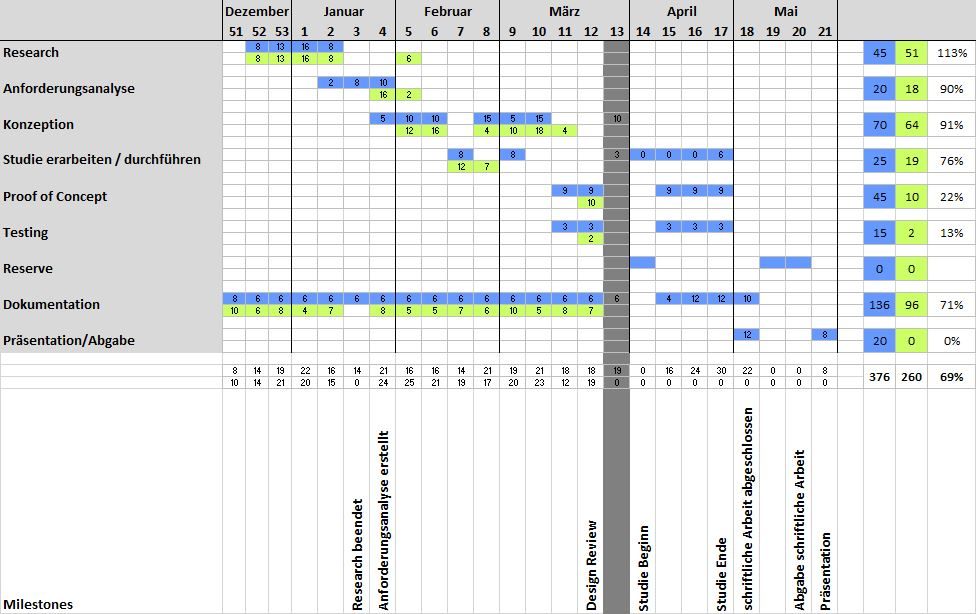
\includegraphics{images/projektplan.jpg}

\newpage

\section{Aufwand}\label{aufwand}

Im Unterkapitel
\protect\hyperlink{rahmenbedingungen-bachelorarbeit}{Rahmenbedingungen
Bachelorarbeit} wurde bereits ausgeführt, dass eine Bachelorarbeit laut
Regelement mindestens 360 Stunden betragen soll. Diese Rahmenbedingung
wurde bei Aufgabenstellung und Aufwandschätzung der Bachelorarbeit
berücksichtigt.

\begin{longtable}[c]{@{}lcl@{}}
\caption{Soll/Ist Analyse}\tabularnewline
\toprule
\begin{minipage}[b]{0.32\columnwidth}\raggedright\strut
\textbf{Arbeitsschritt}
\strut\end{minipage} &
\begin{minipage}[b]{0.24\columnwidth}\centering\strut
\textbf{Soll}
\strut\end{minipage} &
\begin{minipage}[b]{0.35\columnwidth}\raggedright\strut
\textbf{Ist}
\strut\end{minipage}\tabularnewline
\midrule
\endfirsthead
\toprule
\begin{minipage}[b]{0.32\columnwidth}\raggedright\strut
\textbf{Arbeitsschritt}
\strut\end{minipage} &
\begin{minipage}[b]{0.24\columnwidth}\centering\strut
\textbf{Soll}
\strut\end{minipage} &
\begin{minipage}[b]{0.35\columnwidth}\raggedright\strut
\textbf{Ist}
\strut\end{minipage}\tabularnewline
\midrule
\endhead
\begin{minipage}[t]{0.32\columnwidth}\raggedright\strut
Initialisierung
\strut\end{minipage} &
\begin{minipage}[t]{0.24\columnwidth}\centering\strut
10
\strut\end{minipage} &
\begin{minipage}[t]{0.35\columnwidth}\raggedright\strut
\strut\end{minipage}\tabularnewline
\begin{minipage}[t]{0.32\columnwidth}\raggedright\strut
Recherche
\strut\end{minipage} &
\begin{minipage}[t]{0.24\columnwidth}\centering\strut
45
\strut\end{minipage} &
\begin{minipage}[t]{0.35\columnwidth}\raggedright\strut
\strut\end{minipage}\tabularnewline
\begin{minipage}[t]{0.32\columnwidth}\raggedright\strut
Analyse
\strut\end{minipage} &
\begin{minipage}[t]{0.24\columnwidth}\centering\strut
20
\strut\end{minipage} &
\begin{minipage}[t]{0.35\columnwidth}\raggedright\strut
\strut\end{minipage}\tabularnewline
\begin{minipage}[t]{0.32\columnwidth}\raggedright\strut
Konzeption
\strut\end{minipage} &
\begin{minipage}[t]{0.24\columnwidth}\centering\strut
80
\strut\end{minipage} &
\begin{minipage}[t]{0.35\columnwidth}\raggedright\strut
\strut\end{minipage}\tabularnewline
\begin{minipage}[t]{0.32\columnwidth}\raggedright\strut
Prototyp
\strut\end{minipage} &
\begin{minipage}[t]{0.24\columnwidth}\centering\strut
60
\strut\end{minipage} &
\begin{minipage}[t]{0.35\columnwidth}\raggedright\strut
\strut\end{minipage}\tabularnewline
\begin{minipage}[t]{0.32\columnwidth}\raggedright\strut
Dokumentation
\strut\end{minipage} &
\begin{minipage}[t]{0.24\columnwidth}\centering\strut
140
\strut\end{minipage} &
\begin{minipage}[t]{0.35\columnwidth}\raggedright\strut
\strut\end{minipage}\tabularnewline
\begin{minipage}[t]{0.32\columnwidth}\raggedright\strut
Abgabe
\strut\end{minipage} &
\begin{minipage}[t]{0.24\columnwidth}\centering\strut
20
\strut\end{minipage} &
\begin{minipage}[t]{0.35\columnwidth}\raggedright\strut
\strut\end{minipage}\tabularnewline
\begin{minipage}[t]{0.32\columnwidth}\raggedright\strut
\textbf{Total}
\strut\end{minipage} &
\begin{minipage}[t]{0.24\columnwidth}\centering\strut
\textbf{375}
\strut\end{minipage} &
\begin{minipage}[t]{0.35\columnwidth}\raggedright\strut
\textbf{xx}
\strut\end{minipage}\tabularnewline
\bottomrule
\end{longtable}

\newpage

\section{Meilensteine}\label{meilensteine}

Meilensteine sind zum einen sehr wichtig für das Projektmanagement, da
sie den gesamten Ablauf der Bachelorarbeit in mehrere kleine und
überschaubarere Etappen und Zwischenziele einteilen. Dadurch kann auf
dem Weg die Bachelorarbeit erfolgreich umzusetzten immer wieder Inne
gehalten und kontrolliert werden, wie der Stand der Dinge ist, ob die
Richtung geändert werden muss. So bleibt stets der Überblick gewahrt und
das Projekt Bachelorarbeit gerät nicht ausser Kontrolle. \footnote{\autocite{meilensteine}}

\begin{longtable}[c]{@{}ll@{}}
\caption{Meilensteine}\tabularnewline
\toprule
\begin{minipage}[b]{0.37\columnwidth}\raggedright\strut
\textbf{Ende Meilstein}
\strut\end{minipage} &
\begin{minipage}[b]{0.26\columnwidth}\raggedright\strut
\textbf{Meilenstein}
\strut\end{minipage}\tabularnewline
\midrule
\endfirsthead
\toprule
\begin{minipage}[b]{0.37\columnwidth}\raggedright\strut
\textbf{Ende Meilstein}
\strut\end{minipage} &
\begin{minipage}[b]{0.26\columnwidth}\raggedright\strut
\textbf{Meilenstein}
\strut\end{minipage}\tabularnewline
\midrule
\endhead
\begin{minipage}[t]{0.37\columnwidth}\raggedright\strut
bis 10. Januar 2016
\strut\end{minipage} &
\begin{minipage}[t]{0.26\columnwidth}\raggedright\strut
Recherche beendet
\strut\end{minipage}\tabularnewline
\begin{minipage}[t]{0.37\columnwidth}\raggedright\strut
bis 28. Februar 2016
\strut\end{minipage} &
\begin{minipage}[t]{0.26\columnwidth}\raggedright\strut
Anforderungsanalyse beendet
\strut\end{minipage}\tabularnewline
\begin{minipage}[t]{0.37\columnwidth}\raggedright\strut
bis 20. März 2016
\strut\end{minipage} &
\begin{minipage}[t]{0.26\columnwidth}\raggedright\strut
Design Review
\strut\end{minipage}\tabularnewline
\begin{minipage}[t]{0.37\columnwidth}\raggedright\strut
bis 24. April 2016
\strut\end{minipage} &
\begin{minipage}[t]{0.26\columnwidth}\raggedright\strut
Applikation steht zur Verfügung
\strut\end{minipage}\tabularnewline
\begin{minipage}[t]{0.37\columnwidth}\raggedright\strut
bis 8. Mai 2016
\strut\end{minipage} &
\begin{minipage}[t]{0.26\columnwidth}\raggedright\strut
schriftliche Arbeit abgeschlossen
\strut\end{minipage}\tabularnewline
\begin{minipage}[t]{0.37\columnwidth}\raggedright\strut
bis 22. Mai 2016
\strut\end{minipage} &
\begin{minipage}[t]{0.26\columnwidth}\raggedright\strut
Abgabe schriftliche Arbeit
\strut\end{minipage}\tabularnewline
\begin{minipage}[t]{0.37\columnwidth}\raggedright\strut
bis 29. Mai 2016
\strut\end{minipage} &
\begin{minipage}[t]{0.26\columnwidth}\raggedright\strut
Präsentation
\strut\end{minipage}\tabularnewline
\bottomrule
\end{longtable}

\newpage

\section{Termine}\label{termine}

\begin{longtable}[c]{@{}ll@{}}
\caption{Termine der Bachelorarbeit}\tabularnewline
\toprule
\begin{minipage}[b]{0.16\columnwidth}\raggedright\strut
\textbf{Datum}
\strut\end{minipage} &
\begin{minipage}[b]{0.47\columnwidth}\raggedright\strut
\textbf{Termin}
\strut\end{minipage}\tabularnewline
\midrule
\endfirsthead
\toprule
\begin{minipage}[b]{0.16\columnwidth}\raggedright\strut
\textbf{Datum}
\strut\end{minipage} &
\begin{minipage}[b]{0.47\columnwidth}\raggedright\strut
\textbf{Termin}
\strut\end{minipage}\tabularnewline
\midrule
\endhead
\begin{minipage}[t]{0.16\columnwidth}\raggedright\strut
28.10.2015
\strut\end{minipage} &
\begin{minipage}[t]{0.47\columnwidth}\raggedright\strut
Besprechung Aufgabenstellung mit Betreuer
\strut\end{minipage}\tabularnewline
\begin{minipage}[t]{0.16\columnwidth}\raggedright\strut
18.11.2015
\strut\end{minipage} &
\begin{minipage}[t]{0.47\columnwidth}\raggedright\strut
Freigabe der Aufgabenstellung
\strut\end{minipage}\tabularnewline
\begin{minipage}[t]{0.16\columnwidth}\raggedright\strut
9.12.2015
\strut\end{minipage} &
\begin{minipage}[t]{0.47\columnwidth}\raggedright\strut
Kichkoff
\strut\end{minipage}\tabularnewline
\begin{minipage}[t]{0.16\columnwidth}\raggedright\strut
6.01.2016
\strut\end{minipage} &
\begin{minipage}[t]{0.47\columnwidth}\raggedright\strut
Statusmeeting mit Betreuer
\strut\end{minipage}\tabularnewline
\begin{minipage}[t]{0.16\columnwidth}\raggedright\strut
\strut\end{minipage} &
\begin{minipage}[t]{0.47\columnwidth}\raggedright\strut
Statusmeeting mit Betreuer
\strut\end{minipage}\tabularnewline
\begin{minipage}[t]{0.16\columnwidth}\raggedright\strut
\strut\end{minipage} &
\begin{minipage}[t]{0.47\columnwidth}\raggedright\strut
Statusmeeting mit Betreuer
\strut\end{minipage}\tabularnewline
\begin{minipage}[t]{0.16\columnwidth}\raggedright\strut
\strut\end{minipage} &
\begin{minipage}[t]{0.47\columnwidth}\raggedright\strut
Statusmeeting mit Betreuer
\strut\end{minipage}\tabularnewline
\begin{minipage}[t]{0.16\columnwidth}\raggedright\strut
\strut\end{minipage} &
\begin{minipage}[t]{0.47\columnwidth}\raggedright\strut
Designreview
\strut\end{minipage}\tabularnewline
\begin{minipage}[t]{0.16\columnwidth}\raggedright\strut
\strut\end{minipage} &
\begin{minipage}[t]{0.47\columnwidth}\raggedright\strut
Statusmeeting mit Betreuer
\strut\end{minipage}\tabularnewline
\begin{minipage}[t]{0.16\columnwidth}\raggedright\strut
\strut\end{minipage} &
\begin{minipage}[t]{0.47\columnwidth}\raggedright\strut
Abgabe schriftliche Arbeit
\strut\end{minipage}\tabularnewline
\begin{minipage}[t]{0.16\columnwidth}\raggedright\strut
\strut\end{minipage} &
\begin{minipage}[t]{0.47\columnwidth}\raggedright\strut
Präsentation
\strut\end{minipage}\tabularnewline
\bottomrule
\end{longtable}

\newpage

\section{Infrastruktur}\label{infrastruktur}

Im Unterkapitel Infrastruktur sollen die verwendeten Tools erläutert
werden.

\subsection{Quellcode-Verwaltung}\label{quellcode-verwaltung}

Um einerseits eine Datensicherung zu gewährleisten und anderseits die
Änderungen nachvollziehbar abzulegen, wird die Bachelorarbeit mittels
Git und GitHub versioniert. Das Repository \footnote{https://github.com/coffeefan/bachelorarbeit}
ist für den Betreuer, Experten und Auftrageber jederzeit einsehbar.

\subsection{Zeitmanagement}\label{zeitmanagement}

Beim Arbeiten an der Bachelorarbeit kann man sich schnell in details
verlieren. Das Zeitmanagement Tool toggl\footnote{https://toggl.com}
gibt einem schnell ein Feedback zu aktuell verbrauchten Zeit und einen
Überblick um das geplante mit der realen Zeit zu vergleichen.Die
Software ist besonders unter Kreativagenturen und Freelancern beliebt.
Sie präsentiert sich als eine besonders simple Lösung, die die flexible
Zeiterfassung in den Fokus stellt. Der User kann neue Aufgaben mit nur
einem Klick anlegen und die Stoppuhr starten, um Arbeitszeiten
automatisch zu erfassen.

\newpage

\subsection{yUML}\label{yuml}

Um Abläufe, Use Case und andere Uml-Diagramme zu visualisieren bedarf es
ein Tool dass die Diagramm sowohl optisch ansprechend wie aber auch
einfach und schnell anpassbar umsetzt. yUML ist ein gratis online
service über welchen Code und dadurch ziemlich strukturiert ein
UML-Diagramm kreiert werden kann. Der Code welche zum Diagramm führt
kann so einfach als Textdatei abgespeichert werden und wird in dieser
Bachelorarbeit im Github-Repository hinterlegt.

\begin{figure}[htbp]
\centering
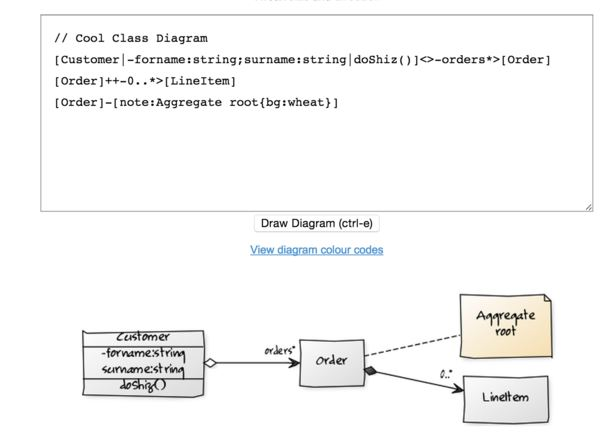
\includegraphics{images/yuml.JPG}
\caption{Screenshot yUML Beispiel Klassendiagramm}
\end{figure}

\newpage

\chapter{Recherche}\label{recherche}

\section{Fachbegriffe}\label{fachbegriffe}

Eine ausführliche Erklärung der Fachbegriffe befindet sich im Anhang
unter dem Kapitel ``\protect\hyperlink{glossar}{Glossar}''.

\section{Erläuterung der
Grundlagen}\label{erluxe4uterung-der-grundlagen}

In diesem Kapitel werden Funktionsweisen und Grundlage ausgeführt, die
als für die Bearbeitung dieser Bachelorthesis herangezogen wurden.

\hypertarget{authentifizierung}{\subsection{Authentifizierung}\label{authentifizierung}}

Authentifizierung - beglaubigen, die Echtheit von etwas bezeugen
\footnote{\autocite{duden}}

Eine Person oder Objekt eindeutig zu \textbf{authentifizieren} bedeute
zu ermitteln ob die oder derjenige auch der ist als welcher er sich
ausgibt. \footnote{\autocite{authentifizierungsdef}} Dies unterstreicht
auch die Ableitung des Wortes vom Englischen Verb \emph{authenicate},
was auf Deutsch sich als \emph{echt erweisen, sich verbürgen,
glaubwürdig sein} bedeutet. Das bekannteste Verfahren der
Authenfizierung ist die Eingabe von Benutzernamen und Passwort. Weiter
ist die PIN-Eingabe bei Bankautomaten oder Mobiletelefon häufig
verbreitet. Die Möglichkeiten der Authentifizierung nahe zu grenzenlos.
\footnote{\autocite{authentifizierungsdeforg}}

\subsection{Autorisierung}\label{autorisierung}

Autorisierung - Befugnis, Berechtigung, Erlaubnis, Genehmigung
\footnote{\autocite{duden}}

Wenn die
Authenfizierung\protect\hyperlink{authentifizierung}{Authentifizierung}
erfolgreich war erteilt das System die Autorisierung. Dabei wird der
Person oder Objekt erlaubt bestimmte Aktionen/Zugriffe durchzuführen.
Meist verfügen unterschiedliche Benutzer eines Systems über verschiedene
Zugriffsrechte. Die korrekte Zuweisung der individuellen Rechte ist
ebenfalls Bestandteil der Autorisierung.

Der Begriff Authentifizierung wird vielfach mit dem Begriff
Autorisierung verwechselt. Die Authentifizierung wird vom Benutzer
initiiert. Sie dient dem Nachweis, zur Ausübung bestimmter Rechte befugt
zu sein. Die anschließende Autorisierung erfolgt automatisch durch das
System selbst. Im Zuge der Autorisierung werden dem Benutzer seine
Zugriffsrechte zugewiesen. \autocite{authentifizierungsdeforg}

\newpage

\hypertarget{oauth}{\subsection{OAuth}\label{oauth}}

OAuth ist ein Protokoll. Es erlaubt sichere API-Autorisierungen.

\subsubsection{Das Bedürfnis nach
OAuth}\label{das-beduxfcrfnis-nach-oauth}

2006 implementiere Blaine Cook OpenID für Twitter. Ma.gnolia erhielt
dabei ein Dashboard welches sich durch OpenID autorisieren lies. Deshalb
suchten die Entwickler von Ma.gnolia und Blaine Cook eine Möglichkeit
OpenID auch für die Verwendung von APIs zu gebrauchen. Sie diskutierten
Implementierungen und stellten fest, dass es keinen offenen Standart für
API-Access Delegation gab. So fingen sie an den Standard zu entwickeln.
2007 entstand daraus eine Google Group. Am 3. October 2007 war dann der
OAuth Core 1.0 bereits released worden.

\subsubsection{Funktionalität von
OAuth}\label{funktionalituxe4t-von-oauth}

Ein Programm/API (Consumer) stellt über das OAuth-Protokoll einem
Endbenutzer(User) Zugriff (Autorisierung) auf seine
Daten/Funktionalitäten zur Verfügung. Dieser Zugriff wird von einem
anderen Programm (Service) gemanagt. Das Konzept ist nicht generell neu.
OAuth ist ähnlich zu Google AuthSub, aol OpenAuth, Yahoo BBAuth,
Upcoming api, Flickr api, Amazon Web Services api. OAuth studierte die
existierenden Protokolle und standardisiert und kombinierte die
existierende industriellen Protokolle. Der wichtigste Unterschied zu den
existierenden Protokollen ist, das OAuth sowohl offen ist und es
geschafft hat genügend Einsatzgebiete zu finden um als Standard zu
gelten. Jeden Tag entstehen neue Webseite welche neue Funktionalitäten
und Services offerieren und dabei Funktionalitäten von anderen Webseiten
brauchen. OAuth stellt dem Programmierer einerseits eine standardisierte
Implementierung zur Verfügung. Anderseites erhält der Endbenutzer dank
dieses Protokolls die Möglichkeit Teile seiner Funktionalität/Daten bei
einem anderen Anbieter zur Verfügung zu stellen. Zum Beispiel bei
Facebook OAuth kann der Endbenutzer seine Posts zur Verfügung stellen
nicht aber seine Freunde bekannt geben.

Dank der weiten Verbreitung gibt es nun in allen bekannten
Programmiersprachen eine Implementierung sowohl von Client wie auch vom
Server. Weitere Infos dazu unter oauth.net\href{http://oauth.net/2/}{1}

\newpage

\section{Ähnliche Produkte auf dem
Markt}\label{uxe4hnliche-produkte-auf-dem-markt}

Dieses Unterkapitel erläutert existierenden Produkte auf dem Markt.

\subsection{OAuth-Provider}\label{oauth-provider}

Die grössten \protect\hyperlink{oauth}{OAuth}-Provider wie Google,
Facebook und Twitter erziehlen eine weiter Verbreitung weltweit:

\begin{figure}[htbp]
\centering
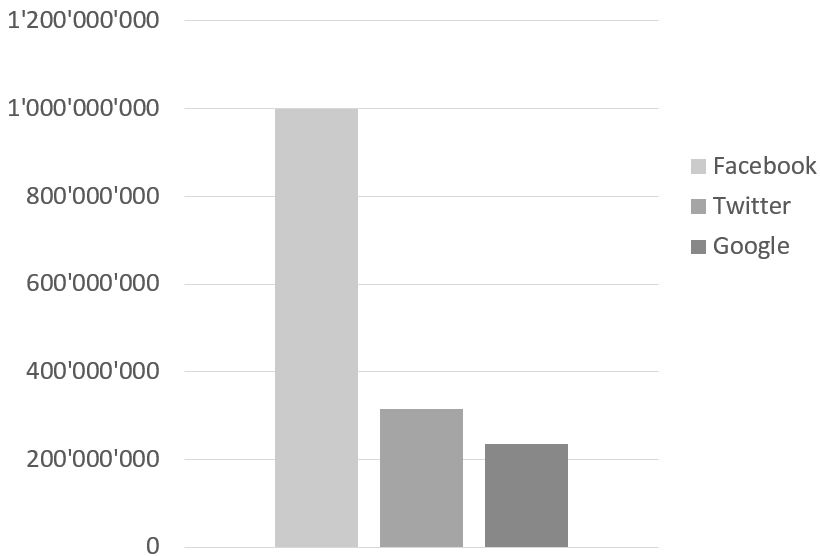
\includegraphics{images/excel-statistik/socialmedia-aktivenutzer.jpg}
\caption[Aktive Nutzer Weltweit ]{Aktive Nutzer Weltweit
\footnotemark{}}
\end{figure}
\footnotetext{Das Statistik wurde basierend auf den Daten von
  socialmedia-institute \autocite{smi}erstellt. Facebook und Twitter
  Daten sind am 5. November 2015 und die Google Daten sind im 2014
  erhoben worden.}

Ganze \emph{78\%} \autocite{goldbachsocial} der Schweizer Bevölkerung
nutzten SocialMedia und besitzen dadurch einen OAuth-Account:

\begin{figure}[htbp]
\centering
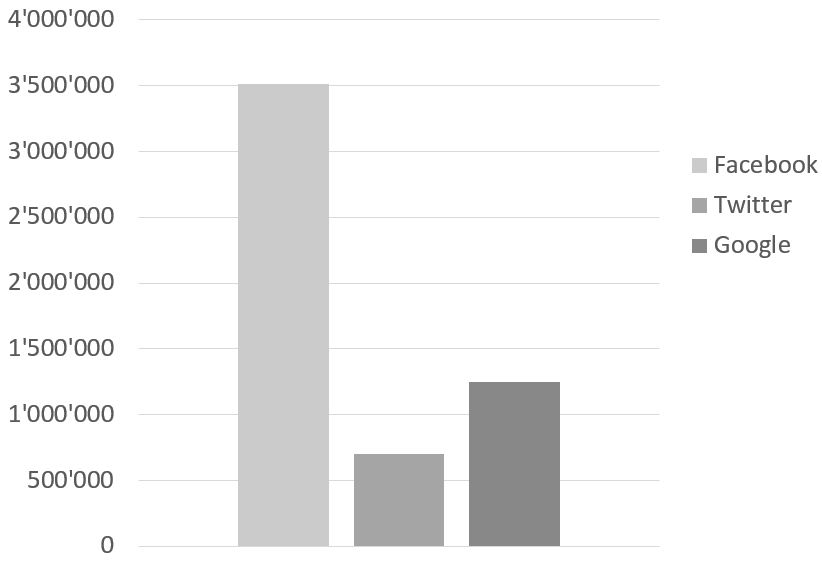
\includegraphics{images/excel-statistik/socialmedia-schweiz.jpg}
\caption[Anzahl Schweizer Nutzer ]{Anzahl Schweizer Nutzer
\footnotemark{}}
\end{figure}
\footnotetext{Das Statistik wurde basierend auf den Daten von Goldbach
  Interactive \autocite{goldbachsocial} generiert. Die Daten sind im
  März 2015 erhoben.}

\newpage

\subsubsection{Vorteile}\label{vorteile}

Mindestes 78\% der Schweizer Bevölkerung besitzt bereits einen OAuth
Account. Das Protokoll ist ein etablierter Standard.

\subsubsection{Nachteile}\label{nachteile}

Mehrfachregistrierungen sind möglich. Jenach OAuth-Provider werden
verschiedene Daten zur Verfügung gestellt. Pro OAuth Provider kann man
sich registrieren einen Abgleich der verschiedenen OAuth Provider wird
vom \protect\hyperlink{oauth}{OAuth}-Protokoll nicht zur Verfügung
gestellt. Ein Teil der Bevölkerung müsste sich vor Nutzung noch
registrieren. Die Implementierung ist trotz vielen Libaries nicht ohne
tiefere Programmierkenntnisse möglich.

\newpage

\subsection{playbuzz.com}\label{playbuzz.com}

Youtube von Google ist im Jahr 2015 mit Abstand die meist verbreiteste
Videopublishing-Plattform\footnote{\autocite{statista}}. Medienhäuser
nutzen Youtube um einfach Ihren Artikel mit einem Video zu ergänzen.
Neben der einfachen Integration profitieren die Medienhäuser von der
zusätzlichen Verbreitung über youtube.com und der einfachen viralen
Verbreitungsmöglichkeiten von youtube. PlayBuzz möchte das Youtube für
Votings, Quiz und ähnlicher Embeded Content zu werden. Neben MTV, Focus,
Time oder Bild verwendet seit Herbst 2015 auch ein grosses Medienhaus
der Schweiz die Plattform. Tamedia erfasst neu auf 20minuten Votings und
Umfragen mit PlayBuzz.

2012 wurde Playbuzz von Shaul Olmert (Sohn des Premie Minster von Israel
Ehuad Olmert) und Tom Pachys ins Leben gerufen. Der offizielle Launch
war im Dezember 2013. Im Juni 2014 wurde Playbuzz bereits das 1. Mal
unter den Top 10 Facebook Shared Publishers aufgelistet. Im Juni 2014
konnte Playbuzz bereits 70 millionen unique views aufweisen. Im
September 2014 kamen 7 von den 10 Top Shares auf Facebook laut
forbes.com von Playbuzz. Playbuzz setzt nach eigenen Angaben auf Content
wie Votes und Quizes welcher gerne Viral geteilt wird und ermöglicht
Endnutzer und Redaketeueren einfache Verwendung. \footnote{\autocite{t3nplaybuzz}}
\footnote{\autocite{playbuzz}}

\subsubsection{Vorteile}\label{vorteile-1}

Playbuzz ist kostenlos und lässt sich einfach integrieren. Durch
Verwendung von Playbuzz kann die Verbreitung des eigenen Inhalts
gesteigert werden. Die Verwaltungsoberfläche und Reports sind
übersichtlich und einfach zu bedienen.

\subsubsection{Nachteile}\label{nachteile-1}

Der Verweis auf Playbuzz ist ersichtlich. Auch beim Posten auf den
SocialMedia-Kanälen ist die Herkunft von Playbuzz offensichtlich. Die
Möglichkeiten in Funktionalität und Design haben Grenzen. Individuelle
Erweiterungen sind nicht einfach möglich.

\newpage

\subsection{WebSMS.com
Zwei-Faktor-Authentifizierung}\label{websms.com-zwei-faktor-authentifizierung}

WebSMS.com bittet eine Zwei-Faktor-Authentifizierung über SMS an. Der
User gibt seine Mobilnummer in der Webmaske der Schnittstelle ein und
erhält einen Code welcher der User danach in der Webschnittstelle
eingibt. Dadurch kann sichergestellt werden dass der User zur
eingegebenen Mobilenummer passt. Der Service kostet monatlich 20 CHF und
weitere 0.08 CHF pro SMS \footnote{Die Kosten sind am 28. Dezember 2015
  unter folgendem Link abgerufen worden:
  https://websms.ch/preise\#at-preisuebersicht}

Die Stärke und Sicherheit dieses Service ist direkt mit mit dem Umgang
von Mobilenummern/SIM-Karten und dessen Authentifizierung verbunden.

Seit 1. Juli 2004 müssen auch bei Prepaid-Karten in der Schweiz
Personalien hinterlegt werden.\footnote{Meldung des UVEKS über
  Gesetzesänderung: \autocite{uvek}} Dadurch ist eine eindeutige
Authentifizierung über Mobilennummer gewährleistet. Die
Mobilefunkanbieter schrenken die Anzahl SIM-Karten auf maximal 5 pro
Person ein. Dieses Maximum konnte aber auf den Webseiten der Anbieter
nicht direkt gefunden werden. Daher galt es den Wert zu untersuchen und
mögliche abweichungen ausfindig zu machen.

\subsubsection{Swisscom}\label{swisscom}

Die Swisscom hat kein öffentlich zugängigliches Dokument welches die
maximale Anzahl SIM-Karten pro Person beschreibt. Mündlich durch das
Verkaufspersonal des Swisscom-Shops Zürich HB Dezember 2015 und im
Chatprotokoll \footnote{Chat-Protokoll Swisscom 12.Februar 2016
  http://bit.ly/swisscom-chat} wurde der Wert bestätigt. Es hingewiesen,
dass nicht ein Dokument mit dieser Zahl vorhanden ist.

\paragraph{Selbstversuch}\label{selbstversuch}

Es wurde versucht bei zwei unabhängigen Handyanbieter mehr als 5
Swisscom-Perpaid-Abos abzuschliessen. Dabei wurden von Thomas Bachmann
über 4 Wochen verteilt bei dem Anbieter Interdiscount im Manor
Winterthur bei verschiedenem Kaufspersonal ein Prepaidhandy eingekauft.
Beim Einkauf des 6. Handys wurde der Verkauf von der Kasse abgelehnt.
Die Fehlermeldung der Kasse beinhaltete den Hinweis, dass sich die
Nummer nicht erneut auf den Kunden registrieren lassen kann, da er schon
5 SIM Karten bei der Swisscom besitzt. Christian Bachmann kaufte über 2
Wochen verteilt bei dem Anbieter Migros Electronics in der Migros
Limmat, Interdiscount im Manor Winterthur, Interdiscount im Zürich HB
bei verschiedenem Kaufspersonal ein Swisscom Prepaidhandy. Beim Einkauf
des 6. Handys wurde der Verkauf von der Kasse abgelehnt. Die Nummer
liess sich nicht erneut auf den Kunden registrieren, da er schon 5 SIM
Karten bei der Swisscom besitzt.

\subsubsection{Sunrise}\label{sunrise}

Die Sunrise hat nach Rücksprache ein PDF mit Ihren Bestell- und
Lieferbedingunge zugesendet.\footnote{Kopie Bestell- und
  Lieferbedingungen http://bit.ly/sunrise-bedienungen} Die maximale
Anzahl SIM-Karten ist in diesen Bestell- und Lieferbedingungen
festgelegt. Auch die Sunrise hat das Maximum auf 5 pro Person
festgelegt.

\subsubsection{SALT}\label{salt}

Bei der Die Firma SALT konnte mir ebenfalls kein Dokument mit der
Kennzahl gegeben werden. SALT stellt vergibt ihrer schriftlichen
Auskunft \footnote{E-Mail von Salt 13.Februar 2016
  http://bit.ly/salt-email} pro Person maximum 3 SIM Karten.

\subsubsection{Vorteile}\label{vorteile-2}

Die mehrfache Registrierung ist auf maximal 5 beschränkt. Durch die
Kosten für eine SIM-Karte/Mobilenummer wird der Wert zusätzlich
gemindert. Bei Missbrauch kann der User eindeutig identifiziert werden.
Eine Automatisierung ist nahe zu unmöglich.

\subsubsection{Nachteile}\label{nachteile-2}

Der Versand von SMS verursacht Kosten. Die Implementation bedarf hohes
technisches Know-How.

\newpage

\section{Grundlegende
Sicherheitsprinzipien}\label{grundlegende-sicherheitsprinzipien}

In diesem Unterkapitel werden die Grundlagen der Sicherheitsprinzipien
vermittelt auf denen eine Authentifizierungssoftware aufgebaut werden
kann.

\subsection{KISS}\label{kiss}

\textbf{K}eep \textbf{I}t \textbf{S}tupid \emph{and} \textbf{S}imple

Ein verbreitetes Problem unter Software Engineers und Programmier heute
ist, dass sie dazu tendiert wird, Probleme zu kompliziert und
verschachtelt zu lösen. 8-9 von 10 Entwickeln machen den Fehler,
Probleme zu wenig auseinander zu brechen und alles in einem grossen
Programm zu lösen. Anstatt es in kleinen Paketen verständlich zu
programmieren.{[}\^{}apachekiss{]}

Die folgenden Punkte listen die Vorteile für Software Entwickler bei
verwenden von Kiss auf:

\begin{itemize}
\tightlist
\item
  Mehr Probleme sollen schneller gelöst werden
\item
  Der Entwickler kann komplexe Probleme in wenigen Zeilen Code lösen
\item
  Die Codequalität steigt
\item
  Der Entwickler kann grössere System erstellen und unterhalten
\item
  Der Code wird flexibler werden, einfach wieder zu verwenden und zu
  modifizieren
\item
  Die Zusammenarbeit in grösseren Entwicklerteams und Projekten wird
  vereinfacht da der Code bei allen ``stupid simple'' ist
\end{itemize}

\subsubsection{KISS fördert die
Sicherheit}\label{kiss-fuxf6rdert-die-sicherheit}

Die Begründung warum KISS die Sicherheit fördert, liefert Saltzer und
Schroeder: Ungewollte Zugriffspfade können nur durch zeilenweise
Codeinspektion entdeckt werden und die wiederum setzt voraus, dass
Designs einfach und klein sein sind. Designs müssen so beschaffen sein,
dass sie abgeschlossene Bereiche enthalten, über die konkrete und
sichere Aussagen über Zugriffsmöglichkeiten und Effekte getroffen werden
können. {[}\^{}sicheresysteme\_93{]}

\subsection{Default-is-deny}\label{default-is-deny}

Ob eine Person oder Programm Zugriff auf Daten/Funktionen haben, sollte
nicht durch Verbote sondern durch explizite Erlaubnis geregelt werden.
Dies bedeutet solange keine explizite Erlaubnis gesetzt ist, kann das
Programm oder die Person nicht auf die Daten oder Funktionen zugreifen.
You \emph{deny} it. So simpel und logisch diese Idee klingt, umso
verwunderlich ist wie viele Organisationen und Entwicklungsfirma nicht
dieses vorgehen verwenden. z.B. Filesysteme setzten auf Verbote anstatt
auf explizite Erlaubnise.{[}\^{}sicheresysteme\_94{]}
{[}\^{}defaultdeny{]}

\subsection{Open Design}\label{open-design}

Abgeleitet von der Kryprotografie: Nicht das Design der Software sollte
die Sicherheit sein, sondern der verwendete Schlüssel. Dieses Konzept
gilt es in der Softwareentwicklung und Systemtechnik nur bedingt
einzuhalten. Die Software soll nach dem Ansatz entworfen werden.
Mindestens intern soll das Software-Design durch einen Design-Review
Prozess analysiert werden. In manchen Fällen macht es jedoch das
Softwaredesign geheimzuhalten um einem Angreifer nicht zu viele
Informationen zur Verfügung zu stellen. {[}\^{}sicheresysteme\_95{]}

\subsection{Zusammenfassung der
Sicherheitsprinzipien}\label{zusammenfassung-der-sicherheitsprinzipien}

Die wichtigsten Sicherheitsprinzipien zusammengefasst:

\begin{itemize}
\tightlist
\item
  Software muss aus kleinen, isolierten Einheiten aufgebaut werden,
  deren externe Beziehungen am Interface deutlich werden. Damit wird
  sowohl praktische Schadensreduzierung durch Isolation als auch eine
  schnelle und einfache Sicherheitsanalyse möglich.
\item
  Zugriffsentscheidungen dürfen nur auf der Basis expliziter, minimaler
  und keinesfalls durch immer und global verfügbare Permissions fallen.
\item
  Das Softwaredesign von Applikationen sollte wenn möglich öffentlich
  sein. Zumindest sollte ein interner Review-Prozess stattfinden, in
  dessen Verlauf eine Sicherheitsanalyse durch nicht an der Entwicklung
  Beteiligte erstellt wird.
\end{itemize}

{[}\^{}sicheresysteme\_93{]} : \autocite[ pp.93]{sicheresysteme}
{[}\^{}sicheresysteme\_94{]} :\autocite[ pp.94]{sicheresysteme}
{[}\^{}sicheresysteme\_95{]} :\autocite[ pp.95]{sicheresysteme}
{[}\^{}apachekiss{]}: \autocite{apachekiss} {[}\^{}defaultdeny{]}:
\autocite{defaultdeny}

\section{Authetentifizierungskomponenten}\label{authetentifizierungskomponenten}

Die Authentifizierung kann mit verschiedenen Komponenten durchgeführt
werden. Folgend gilt es die Komponenten zu erklären.

\subsection{Captcha}\label{captcha}

Captcha - Test, mit dem festgestellt werden kann, ob sich ein Mensch
oder ein Computer eines Programms bedient \footnote{\autocite{duden}}

Im Jahre 2000 wurde das Captcha an der Carnegie Mellon University
erfunden. Captcha steht für \textbf{C}ompletely \textbf{A}utomated
\textbf{P}ublic \textbf{T}uring test to tell \textbf{C}omputers and
\textbf{H}umans \textbf{A}part. Luis von Ahn, Professor der
Entwickler-Gruppe, erklärte die Dringlichkeit von Captcha damals so:
``Anybody can write a program to sign up for millions of accounts, and
the idea was to prevent that''. **** \footnote{\autocite{captcha}}

\subsubsection{Captcha Zahlen}\label{captcha-zahlen}

In 2014 wurden 200 Million Captchas pro Tag eingegeben. Dabei braucht
ein User durchschnittlich 10 Sekunden das entspricht 500'000
Stunden.\footnote{Die statistischen Daten wurden von Google 2014 in
  ihrem Blog publiziert \autocite{googlecaptcha}}

\begin{figure}[htbp]
\centering

\includegraphics{images/captcha.png}
\caption{Beispiele von Captchas \emph{Quelle:drupal.org}}
\end{figure}

\subsection{Zweiweg Authentifizierung}\label{zweiweg-authentifizierung}

Die Zwei-Faktor-Authentifizierung wird häufig 2FA genannt. Der User wird
mittels zweier unabhängigen Faktoren identifiziert. Der Begriff Faktor
umschreibt dabei eine Komponente oder Authentifizierungsmethode.
{[}\^{}cnet-2fa{]}

Die Zwei-Faktor-Authentifizierung ist in der Schweiz durch das E-Banking
bekannt geworden. Der User gibt als 1. Faktor Username/Vertragnummer und
Passwort ein. In einem 2. Schritt gibt er vom System gewünschten Code
aus der Codekarte oder des elektirschen Rechners als 2. Faktor ein. Im
Alltag bei einem Einkauf im Detailhandel authentifiziert sich der
EC-Karten Chip als 1. Faktor. Als 2. Faktor hat sich der Kunde ein
Passwort auswendig gemerkt welches er eingibt.

Diese 2 Faktor Authentifizierung hatte die Entwicklung und Förderung der
Vielfalt von Faktoren/Komponenten zu folge von welchen wir nun für
unsere Authentifizierung profitieren können:

\subsection{E-Mail Bestätigungs-Code}\label{e-mail-bestuxe4tigungs-code}

Im Registrationsprozess ist das Erhalten eines E-Mails mit
Bestätigungs-Code zum quasi Standart geworden. Durch diese Methodik kann
man garantieren, dass die angegebene E-Mail Adresse auch tatsächlich
existiert und der User darauf Zugriff hat. Der User soll also auch bei
der Authentifizierungsschnittstelle seine E-Mail eintragen und erhält
dann umgehend den Bestätigungslink an seine E-Mail Adresse zugesandt.

\subsubsection{Automatisierungsmöglichkeit}\label{automatisierungsmuxf6glichkeit}

Das automatische Auslesen von E-Mails ist möglich. Jedoch ist der
Aufwand dafür sehr hoch.

\subsubsection{Mehrfach Teilnahme}\label{mehrfach-teilnahme}

Ein User kann verschiedene E-Mail Adressen besitzen. Dass Erstellen von
neuen E-Mail Adressen ist mit Aufwand verbunden. Aber einfach möglich.

Anbieter wie 10-Minutes Mail \footnote{10-Minute Mail
  \autocite{10minutemail}} stellen auf Knopfdruck für einige Minuten
eine temporäre E-Mail Adresse zur Verfügung. Dadurch können schnell
einige E-Mail Adressen erstellt werden. Diese Domains müssen über eine
aufwendige Blacklist gefiltert werden oder durch zeitversetztes
Bestätigungsmail ausgehebelt werden.

\subsubsection{Kosten}\label{kosten}

Das Versenden von E-Mails über einen SMTP Server ist generell kostenlos.
Bei hohem Gebrauch dieser Komponente lohnt es sich die E-Mails über eine
professionelle Inrastruktur für Massenversendung zu versenden und
analysieren. Beispiele dafür sind Mailchimp \footnote{www.mailchimp.com}
oder Sendgrid \footnote{sendgrid.com}

\subsection{SMS Bestätigungs-Code}\label{sms-bestuxe4tigungs-code}

Das Konzept des im einem vorherigen Kapitel Anbieters WebSMS soll von
der Authentifizierungsschnittstelle ebenfalls implementiert werden. Der
User gibt im 1. Schritt seine Mobilenummer ein. Er hält dann einen Code
per SMS zu gesandt. Im 2. Schritt gibt der User der erhaltene Mobilecode
im Webform ein und bestätigt so, dass ihm die Mobilenummer gehört. Zum
Versenden der SMS ist ein SMS-Gateway nötig.

\subsubsection{Automatisierungsmöglichkeit}\label{automatisierungsmuxf6glichkeit-1}

Die Automatisierung kann als nicht möglich eingestuft werden

\subsubsection{Mehrfach Teilnahme}\label{mehrfach-teilnahme-1}

Die mehrfache Teilnahme wurde bereits im Kapitel zum Anbieter WebSMS
eingehenden behandelt. Daraus resultierte, dass in der Schweiz maximal 5
Mobilenummern pro Anbieter und Person bezogen werden können.

\subsubsection{Kosten}\label{kosten-1}

Je nach SMS-Gateway, Mobileanbieter des Empfängers und
Verwendungsintensität belaufen sich der Versand eines SMS zwischen 0.04
CHF und 0.15 CHF \footnote{Die Preise wurden am 1. März 2016 auf
  aspsms.ch/instruction/prices.asp, tropo.com/pricing und
  twilio.com/sms/pricing abgefragt}

\subsection{Telefonanruf mit
Bestätigungscode}\label{telefonanruf-mit-bestuxe4tigungscode}

Nacheingabe der Telefonnummer oder Mobilenummer erhält der User einen
digitalen Anruf. Die Computerstimme liest dem User einen Code vor,
welcher er danach in der Webpage einggibt.

\subsubsection{Automatisierungsmöglichkeit}\label{automatisierungsmuxf6glichkeit-2}

Die Automatisierung kann als nicht möglich eingestuft werden

\subsubsection{Mehrfach Teilnahme}\label{mehrfach-teilnahme-2}

Die Teilnahmeanzahl ist von den vorhandenen Telefonanschlüssen abhängig
und daher nur eingschrenkt möglich.

\subsubsection{Kosten}\label{kosten-2}

Die Kosten berechnen sich bei den analysierten Anbietern basierend auf
einer geringen Monatspauschle zwischen CHF 1.00 und CHF 2.00 und Kosten
pro Minute je nach Telefonanbieter des Empfängers und Voicegateway
zwischen CHF 0.10 und CHF 0.65.\footnote{Die Preise wurden am 1. März
  2016 auf nexmo.com/products/voice/, tropo.com/pricing und
  twilio.com/voice/pricing abgefragt}

\subsection{Postversand}\label{postversand}

Wie kann sichergestellt werden, dass eine Person auch tatsächlich am
angegebenen Ort wohnt? Im Telefonbuch digital oder analog waren früher
fast alle Personen erfasst. Immer weniger Personen haben heute einen
Fixanschluss und einige lassen Ihre Nummern nicht mehr eintragen. Nur
vereinzelte Personen tragen Ihre mobile Telefonnumer und Adresse im
Telefonbuch ein. Google steht vor dem gleichen Problem mit Ihrem Produkt
Google Maps. In Google Maps sollen schnell neue Firmendaten,
Veranstaltungslocations oder andere Adresseintröge erfasst werden
können. Doch sollen Betrügern oder Spassvögel daran gehindert werden
Falscheinträge zu machen. Daher versendet Google zur Verifikation
einfach einen Code per Brief bzw.Postkarte an die Adresse.\footnote{\autocite{googlebusiness}}
Das simple Konzept kann auch für den Authentifizierungsschnittstelle
umsetzt werden um die Adresse eindeutig zu verifizieren. Einen Haken hat
dieses Konzept jedoch. Jemand muss den Brief ausdrucken, in ein Couvert
legen, frankieren und per Post versenden. Dieser Jemand kann als Service
z.b. beim schweizer Startup pingen.com eingekauft werden.

\subsubsection{Automatisierungsmöglichkeit}\label{automatisierungsmuxf6glichkeit-3}

Die Automatisierung kann als nicht möglich eingestuft werden.

\subsubsection{Mehrfach Teilnahme}\label{mehrfach-teilnahme-3}

Die Teilnahmeanzahl ist von den vorhandenen Adressanschriften abhängig
und daher nur eingschrenkt möglich.

\subsubsection{Kosten}\label{kosten-3}

Die Kosten berechnen sich für den Versand in der Schweiz bei dem
analysierten Anbietern je nach Druck und Versandart des Empfängers
zwischen CHF 1.20 und CHF 1.65.\footnote{Die Preise wurdem am 10. März
  2016 auf pingen.com abgefragt}

\subsection{Browser Fingerprints}\label{browser-fingerprints}

Der Fingerabdruck ist aus der Kriminaltechnik nicht mehr wegzudenken.
Bereits vor 2000 Jahren haben Chinesen ihre Schuldscheine mit
Fingerabdrücke unterzeichnet. Es sollten über 19 Jahrhunderte gehen bis
der Fingerabdrücke auch in der Kriminaltechnik ein gesetzt wurde. Seit
über 100 Jahren 1913 ist der Fingerabdruck auch im Dienst der Schweizer
Eidgenossenschaft. Im Gegensatz zur DNA unterscheidet sich der
Fingerabdruck bei Zwillingen klar auch wenn ähnliche Merkmale erkennbar
sind. Bereits nach nur 4 Monaten Schwangerschaft sind die Muster der
Papilarleisten beim Embryo festgelegt. Der einzigartige Fingerabdruck
des Menschen ist fertig. Dieses Muster ändert sich bis zur Auflösung des
Körpers nach dem Tod nicht mehr. \footnote{\autocite{derfingerabdruck}}

\begin{figure}[htbp]
\centering
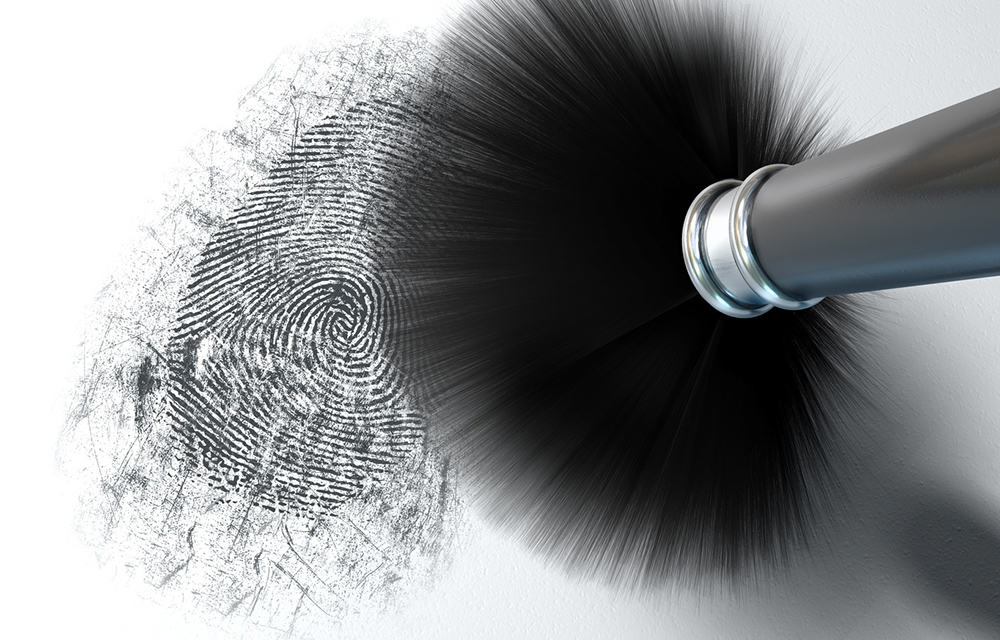
\includegraphics{images/fingerabdruck.jpg}
\caption{Fingerabdruck Mit Kohlepulver werden Fingerabdrücke sichtbar
gemacht und auf Klebefolie gesichert \emph{Quelle:phi-hannover.de}}
\end{figure}

Der Fingerabdruck eignet sich zur Authentifizierung einer Person durch
folgende Merkmale: - Der Fingerabdruck ist eindeutig - Der Fingerabdruck
ist über den Tod hinaus beständig - Der Fingerabdruck ist von aussen
einfach ``abrufbar''. Er ist von blossem Augenn sichtbar und wir
hinterlassen das Muster der Papilarleiste auf Gegenständen wie Glas.

\subsubsection{Fingerabdruck des
Browsers}\label{fingerabdruck-des-browsers}

Im Gegensatz zum Datenschutz wäre es aus Sicht der eindeutigen
Identifikation wünschenswert, wenn digitale Personen oder deren Geräte
auch einen Fingerabdruck von sich geben würde, der sowohl eindeutig,
beständig und abrufbar ist. Immer wieder versuchten unter dem Thema
``Browser Fingerprint'' Personen ein Verfahren zu entwickeln die genau
dies ermöglicht. Microsoft führte laut eigenen Angaben \footnote{\autocite{xpactivation}}
mit Windows XP Produktaktivierung einen Verfahren ein das aus
Prozesser-Typ, Grafikkarten Informationen und Festplatte einen
Fingerabdruck des Geräts erstellt. So konnte bei einer zweiten
Aktivierung mit dem selben Registrationsschlüssel Massnahmen getroffen
werden.

Auch der Browser übermittelt an den Server verschiedene Informationen:

{[}\^{}cnet-2fa{]} {[}\^{}cnet-2fa{]}: \autocite{cnet-2fa}

\chapter{Anforderungen}\label{anforderungen}

Dieses Kapitel beschreibt das Durchführen einer Anforderungsanalyse
festgehalten. Anhand der Anforderungsanalyse sollen die Anforderungen
für die entwickelnden Software ermittelt werden. Die Anforderungen
bilden die Basis für die Architektur, das Softwaredesign, die
Implementationund die Testfälle. Ihnen ist dem entsprechend ein sehr
grosser Stellenwert zuzuschreiben.

\section{Use-Cases}\label{use-cases}

Im Nachfolgenden werden alle UseCases aufgelistet die im Rahmen dieser
Thesis gefunden wurden.

\section{Akteure}\label{akteure}

\begin{longtable}[c]{@{}ll@{}}
\toprule
\begin{minipage}[b]{0.34\columnwidth}\raggedright\strut
\textbf{Akteure}
\strut\end{minipage} &
\begin{minipage}[b]{0.60\columnwidth}\raggedright\strut
\strut\end{minipage}\tabularnewline
\midrule
\endhead
\begin{minipage}[t]{0.34\columnwidth}\raggedright\strut
\textbf{Programmierer}
\strut\end{minipage} &
\begin{minipage}[t]{0.60\columnwidth}\raggedright\strut
Der Programmierer ist der Entwickler der Webseite. Er möchte sein
programmiertes oder sein verwendetes Social-Media Modul mit dem
Authentifizierungsschnittstellen-Service schützen.
\strut\end{minipage}\tabularnewline
\begin{minipage}[t]{0.34\columnwidth}\raggedright\strut
\textbf{User}
\strut\end{minipage} &
\begin{minipage}[t]{0.60\columnwidth}\raggedright\strut
Der User ist der Endkunde. Er nimmt am Social-Media Modul teil und
authentifiziert sich über den Authentifizierungsschnittstellen-Service
\strut\end{minipage}\tabularnewline
\bottomrule
\end{longtable}

\newpage

\subsection{Diagramm}\label{diagramm}

Das Use-Case Diagramm illustriert die nachfolgenden Use Cases. Dadurch
kann rasch ein Überblick über die zu entwickelnde Lösung geschaffen
werden.

\begin{figure}[htbp]
\centering
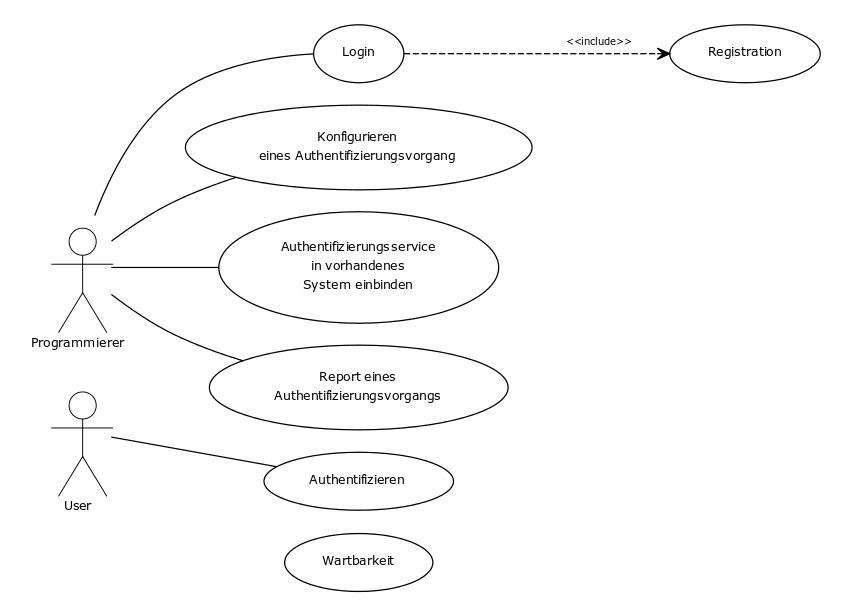
\includegraphics{images/use-case-diagram.png}
\caption{Use-Case Diagram}
\end{figure}

\newpage

\subsubsection{UC-11 Registration}\label{uc-11-registration}

\begin{longtable}[c]{@{}ll@{}}
\toprule
\begin{minipage}[b]{0.34\columnwidth}\raggedright\strut
\textbf{UseCase}
\strut\end{minipage} &
\begin{minipage}[b]{0.60\columnwidth}\raggedright\strut
\strut\end{minipage}\tabularnewline
\midrule
\endhead
\begin{minipage}[t]{0.34\columnwidth}\raggedright\strut
\textbf{Ziel}
\strut\end{minipage} &
\begin{minipage}[t]{0.60\columnwidth}\raggedright\strut
Ein Programmierer ist am Authentifizierungsschnittstellen-Service
registrieren
\strut\end{minipage}\tabularnewline
\begin{minipage}[t]{0.34\columnwidth}\raggedright\strut
\textbf{Beschreibung}
\strut\end{minipage} &
\begin{minipage}[t]{0.60\columnwidth}\raggedright\strut
Ein Programmierer muss sich am Authentifizierungsschnittstellen-Service
registrieren können
\strut\end{minipage}\tabularnewline
\begin{minipage}[t]{0.34\columnwidth}\raggedright\strut
\textbf{Akteure}
\strut\end{minipage} &
\begin{minipage}[t]{0.60\columnwidth}\raggedright\strut
Programmierer
\strut\end{minipage}\tabularnewline
\begin{minipage}[t]{0.34\columnwidth}\raggedright\strut
\textbf{Vorbedingung}
\strut\end{minipage} &
\begin{minipage}[t]{0.60\columnwidth}\raggedright\strut
Keine
\strut\end{minipage}\tabularnewline
\begin{minipage}[t]{0.34\columnwidth}\raggedright\strut
\textbf{Ergebnis}
\strut\end{minipage} &
\begin{minipage}[t]{0.60\columnwidth}\raggedright\strut
Registrierter Programmierer
\strut\end{minipage}\tabularnewline
\begin{minipage}[t]{0.34\columnwidth}\raggedright\strut
\textbf{Hauptszenario}
\strut\end{minipage} &
\begin{minipage}[t]{0.60\columnwidth}\raggedright\strut
Der Programmierer füllt ein Registrationsformular aus und bestätigt
seine E-Mail Adresse
\strut\end{minipage}\tabularnewline
\begin{minipage}[t]{0.34\columnwidth}\raggedright\strut
\textbf{Alternativszenario}
\strut\end{minipage} &
\begin{minipage}[t]{0.60\columnwidth}\raggedright\strut
-
\strut\end{minipage}\tabularnewline
\bottomrule
\end{longtable}

\subsubsection{UC-12 Login}\label{uc-12-login}

\begin{longtable}[c]{@{}ll@{}}
\toprule
\begin{minipage}[b]{0.34\columnwidth}\raggedright\strut
\textbf{UseCase}
\strut\end{minipage} &
\begin{minipage}[b]{0.60\columnwidth}\raggedright\strut
\strut\end{minipage}\tabularnewline
\midrule
\endhead
\begin{minipage}[t]{0.34\columnwidth}\raggedright\strut
\textbf{Ziel}
\strut\end{minipage} &
\begin{minipage}[t]{0.60\columnwidth}\raggedright\strut
Ein Programmierer kann sich beim
Authentifizierungsschnittstellen-Service
\strut\end{minipage}\tabularnewline
\begin{minipage}[t]{0.34\columnwidth}\raggedright\strut
\textbf{Beschreibung}
\strut\end{minipage} &
\begin{minipage}[t]{0.60\columnwidth}\raggedright\strut
Ein Programmierer muss sich am Authentifizierungsschnittstellen-Service
authentifizieren können
\strut\end{minipage}\tabularnewline
\begin{minipage}[t]{0.34\columnwidth}\raggedright\strut
\textbf{Akteure}
\strut\end{minipage} &
\begin{minipage}[t]{0.60\columnwidth}\raggedright\strut
Programmierer
\strut\end{minipage}\tabularnewline
\begin{minipage}[t]{0.34\columnwidth}\raggedright\strut
\textbf{Vorbedingung}
\strut\end{minipage} &
\begin{minipage}[t]{0.60\columnwidth}\raggedright\strut
Der Programmierer ist registriert.
\strut\end{minipage}\tabularnewline
\begin{minipage}[t]{0.34\columnwidth}\raggedright\strut
\textbf{Ergebnis}
\strut\end{minipage} &
\begin{minipage}[t]{0.60\columnwidth}\raggedright\strut
Authentifizierter und eigeloggter Programmierer
\strut\end{minipage}\tabularnewline
\begin{minipage}[t]{0.34\columnwidth}\raggedright\strut
\textbf{Hauptszenario}
\strut\end{minipage} &
\begin{minipage}[t]{0.60\columnwidth}\raggedright\strut
Der Programmierer loggt sich mit E-Mail und Passwort am
Authentifizierungsschnittstellen-Service ein.
\strut\end{minipage}\tabularnewline
\begin{minipage}[t]{0.34\columnwidth}\raggedright\strut
\textbf{Alternativszenario}
\strut\end{minipage} &
\begin{minipage}[t]{0.60\columnwidth}\raggedright\strut
Der Programmierer sendet sich das verpasste Passwort per E-Mail zu.
Erstellt über den im erhaltenden E-Mail enthaltenen Link ein neues
Passwort und loggt sich mit E-mail und dem neuen Passwort am
Authentifizierungsschnittstellen-Service ein.
\strut\end{minipage}\tabularnewline
\bottomrule
\end{longtable}

\subsubsection{UC-21 Konfigurieren eines
Authentifizierungsvorgang}\label{uc-21-konfigurieren-eines-authentifizierungsvorgang}

\begin{longtable}[c]{@{}ll@{}}
\toprule
\begin{minipage}[b]{0.34\columnwidth}\raggedright\strut
\textbf{UseCase}
\strut\end{minipage} &
\begin{minipage}[b]{0.60\columnwidth}\raggedright\strut
\strut\end{minipage}\tabularnewline
\midrule
\endhead
\begin{minipage}[t]{0.34\columnwidth}\raggedright\strut
\textbf{Ziel}
\strut\end{minipage} &
\begin{minipage}[t]{0.60\columnwidth}\raggedright\strut
Es ist eine neuer Authentifizierungsvorgang für ein neus Social
Media-Modul konfiguriert
\strut\end{minipage}\tabularnewline
\begin{minipage}[t]{0.34\columnwidth}\raggedright\strut
\textbf{Beschreibung}
\strut\end{minipage} &
\begin{minipage}[t]{0.60\columnwidth}\raggedright\strut
Der Programmierer kann ein neuer Authentifizierungsvorgang eröffnen
\strut\end{minipage}\tabularnewline
\begin{minipage}[t]{0.34\columnwidth}\raggedright\strut
\textbf{Akteure}
\strut\end{minipage} &
\begin{minipage}[t]{0.60\columnwidth}\raggedright\strut
Programmierer
\strut\end{minipage}\tabularnewline
\begin{minipage}[t]{0.34\columnwidth}\raggedright\strut
\textbf{Vorbedingung}
\strut\end{minipage} &
\begin{minipage}[t]{0.60\columnwidth}\raggedright\strut
Der Programmierer hat sich am System angemeldet
\strut\end{minipage}\tabularnewline
\begin{minipage}[t]{0.34\columnwidth}\raggedright\strut
\textbf{Ergebnis}
\strut\end{minipage} &
\begin{minipage}[t]{0.60\columnwidth}\raggedright\strut
Neuer Authentifizierungsvorgang
\strut\end{minipage}\tabularnewline
\begin{minipage}[t]{0.34\columnwidth}\raggedright\strut
\textbf{Hauptszenario}
\strut\end{minipage} &
\begin{minipage}[t]{0.60\columnwidth}\raggedright\strut
Der Programmierer eröffnet einen neuen Authentifizierungsvorgang. Er
benennt ihn sinnig. Die zu verwende(n) Authentifizierungskomponennten
werden ausgewählt. Bei der Konfiguration unterstützen die Resultate die
Studie den Programmierer für die optimalte Konfiguration. Am Ende der
Konfiguration werden die Akzeptanzkritieren für eine erfolgreiche
Authtentifizierung festgelegt.
\strut\end{minipage}\tabularnewline
\begin{minipage}[t]{0.34\columnwidth}\raggedright\strut
\textbf{Alternativszenario}
\strut\end{minipage} &
\begin{minipage}[t]{0.60\columnwidth}\raggedright\strut
Ein bestehender Authentifizierungsvorgang wird dupliziert
\strut\end{minipage}\tabularnewline
\bottomrule
\end{longtable}

\subsubsection{UC-25 Einbinden in vorhandenes
System}\label{uc-25-einbinden-in-vorhandenes-system}

\begin{longtable}[c]{@{}ll@{}}
\toprule
\begin{minipage}[b]{0.34\columnwidth}\raggedright\strut
\textbf{UseCase}
\strut\end{minipage} &
\begin{minipage}[b]{0.60\columnwidth}\raggedright\strut
\strut\end{minipage}\tabularnewline
\midrule
\endhead
\begin{minipage}[t]{0.34\columnwidth}\raggedright\strut
\textbf{Ziel}
\strut\end{minipage} &
\begin{minipage}[t]{0.60\columnwidth}\raggedright\strut
Die Authentifizierungsschnittstelle kann in ein (bestehendes) System
eingebunden werden
\strut\end{minipage}\tabularnewline
\begin{minipage}[t]{0.34\columnwidth}\raggedright\strut
\textbf{Beschreibung}
\strut\end{minipage} &
\begin{minipage}[t]{0.60\columnwidth}\raggedright\strut
Der Programmierer kann die Authentifizierungsschnittstelle in seinem
System integrieren
\strut\end{minipage}\tabularnewline
\begin{minipage}[t]{0.34\columnwidth}\raggedright\strut
\textbf{Akteure}
\strut\end{minipage} &
\begin{minipage}[t]{0.60\columnwidth}\raggedright\strut
Programmierer
\strut\end{minipage}\tabularnewline
\begin{minipage}[t]{0.34\columnwidth}\raggedright\strut
\textbf{Vorbedingung}
\strut\end{minipage} &
\begin{minipage}[t]{0.60\columnwidth}\raggedright\strut
Der Programmierer hat sich am System angemeldet. Der Programmierer hat
ein neues Authentifizierungsvorgang konfiguriert
\strut\end{minipage}\tabularnewline
\begin{minipage}[t]{0.34\columnwidth}\raggedright\strut
\textbf{Ergebnis}
\strut\end{minipage} &
\begin{minipage}[t]{0.60\columnwidth}\raggedright\strut
Der Programmierer hat eine Möglichkeit die
Authentifizierungsschnittstelle mit seinem konfigurierten
Authentifizierungsvorgangs in seiner Software einzubinden
\strut\end{minipage}\tabularnewline
\begin{minipage}[t]{0.34\columnwidth}\raggedright\strut
\textbf{Hauptszenario}
\strut\end{minipage} &
\begin{minipage}[t]{0.60\columnwidth}\raggedright\strut
Der Programmierer öffnet die Einbindeseite. Es werden ihm alle Schritte
zur Erfolgreichen Einbindung aufgelistet. Der Code liegt
individualisiert vor. Der Programmierer kopiert den Code in sein
Programm
\strut\end{minipage}\tabularnewline
\begin{minipage}[t]{0.34\columnwidth}\raggedright\strut
\textbf{Alternativszenario}
\strut\end{minipage} &
\begin{minipage}[t]{0.60\columnwidth}\raggedright\strut
-
\strut\end{minipage}\tabularnewline
\bottomrule
\end{longtable}

\subsubsection{UC-31 Authentifizieren}\label{uc-31-authentifizieren}

\begin{longtable}[c]{@{}ll@{}}
\toprule
\begin{minipage}[b]{0.34\columnwidth}\raggedright\strut
\textbf{UseCase}
\strut\end{minipage} &
\begin{minipage}[b]{0.60\columnwidth}\raggedright\strut
\strut\end{minipage}\tabularnewline
\midrule
\endhead
\begin{minipage}[t]{0.34\columnwidth}\raggedright\strut
\textbf{Ziel}
\strut\end{minipage} &
\begin{minipage}[t]{0.60\columnwidth}\raggedright\strut
Der User ist authtentifiziert oder der User abgelehnt
\strut\end{minipage}\tabularnewline
\begin{minipage}[t]{0.34\columnwidth}\raggedright\strut
\textbf{Beschreibung}
\strut\end{minipage} &
\begin{minipage}[t]{0.60\columnwidth}\raggedright\strut
Der User probiert sich über den Authentifizierungsschnittstellen-Service
zu authentifizieren um an einem Social-Media Modul teilzunehmen
\strut\end{minipage}\tabularnewline
\begin{minipage}[t]{0.34\columnwidth}\raggedright\strut
\textbf{Akteure}
\strut\end{minipage} &
\begin{minipage}[t]{0.60\columnwidth}\raggedright\strut
User
\strut\end{minipage}\tabularnewline
\begin{minipage}[t]{0.34\columnwidth}\raggedright\strut
\textbf{Vorbedingung}
\strut\end{minipage} &
\begin{minipage}[t]{0.60\columnwidth}\raggedright\strut
Der Programmierer hat den Authentifizierungsvorgang konfiguriert und in
seinem System eingebunden.
\strut\end{minipage}\tabularnewline
\begin{minipage}[t]{0.34\columnwidth}\raggedright\strut
\textbf{Ergebnis}
\strut\end{minipage} &
\begin{minipage}[t]{0.60\columnwidth}\raggedright\strut
Der Authentifizierungsschnittstellen-Service authentifiziert den User
oder lehnt ihn ab.
\strut\end{minipage}\tabularnewline
\begin{minipage}[t]{0.34\columnwidth}\raggedright\strut
\textbf{Hauptszenario}
\strut\end{minipage} &
\begin{minipage}[t]{0.60\columnwidth}\raggedright\strut
Der User wird vom Social Media Modul an den
Authentifizierungsschnittstellen-Service weitergeleitet. Der User
authentifziert sich. Der User kann die Eingabe des Social Media Modul
erfolgreich abschliessen
\strut\end{minipage}\tabularnewline
\begin{minipage}[t]{0.34\columnwidth}\raggedright\strut
\textbf{Alternativszenario}
\strut\end{minipage} &
\begin{minipage}[t]{0.60\columnwidth}\raggedright\strut
Der User wird vom Social Media Modul an den
Authentifizierungsschnittstellen-Service weitergeleitet. Der User wird
vom System abgelehnt. Der User kann die Eingabe des Social-Media Modul
nicht erfolgreich abschliessen.
\strut\end{minipage}\tabularnewline
\bottomrule
\end{longtable}

\subsubsection{UC-41 Report eines
Authentifizierungsvorgangs}\label{uc-41-report-eines-authentifizierungsvorgangs}

\begin{longtable}[c]{@{}ll@{}}
\toprule
\begin{minipage}[b]{0.34\columnwidth}\raggedright\strut
\textbf{UseCase}
\strut\end{minipage} &
\begin{minipage}[b]{0.60\columnwidth}\raggedright\strut
\strut\end{minipage}\tabularnewline
\midrule
\endhead
\begin{minipage}[t]{0.34\columnwidth}\raggedright\strut
\textbf{Ziel}
\strut\end{minipage} &
\begin{minipage}[t]{0.60\columnwidth}\raggedright\strut
Die Verwendung des Authentifizierungsvorgangs ist übersichtlich
dargestellt
\strut\end{minipage}\tabularnewline
\begin{minipage}[t]{0.34\columnwidth}\raggedright\strut
\textbf{Beschreibung}
\strut\end{minipage} &
\begin{minipage}[t]{0.60\columnwidth}\raggedright\strut
Um den Verwendung des Authentifizierungsvorgangs auszuwerten soll ein
Report erstellt werden
\strut\end{minipage}\tabularnewline
\begin{minipage}[t]{0.34\columnwidth}\raggedright\strut
\textbf{Akteure}
\strut\end{minipage} &
\begin{minipage}[t]{0.60\columnwidth}\raggedright\strut
Programmierer
\strut\end{minipage}\tabularnewline
\begin{minipage}[t]{0.34\columnwidth}\raggedright\strut
\textbf{Vorbedingung}
\strut\end{minipage} &
\begin{minipage}[t]{0.60\columnwidth}\raggedright\strut
Der Programmierer hat sich am System angemeldet. Der Programmierer hat
ein neues Authentifizierungsvorgang konfiguriert. (Der
Authentifizerungsvorgang ist eingebunden und verwendet worden)
\strut\end{minipage}\tabularnewline
\begin{minipage}[t]{0.34\columnwidth}\raggedright\strut
\textbf{Ergebnis}
\strut\end{minipage} &
\begin{minipage}[t]{0.60\columnwidth}\raggedright\strut
Report eines Authentifizierungsvorgangs
\strut\end{minipage}\tabularnewline
\begin{minipage}[t]{0.34\columnwidth}\raggedright\strut
\textbf{Hauptszenario}
\strut\end{minipage} &
\begin{minipage}[t]{0.60\columnwidth}\raggedright\strut
Nach Beenden eines Quizes, Votings, Wettbewerbs logt sich der
Programmierer im System ein und generiert einen automatisierten Report
um die Verwendung des Authentifizierungsvorgangs auszuwerten.
\strut\end{minipage}\tabularnewline
\begin{minipage}[t]{0.34\columnwidth}\raggedright\strut
\textbf{Alternativszenario}
\strut\end{minipage} &
\begin{minipage}[t]{0.60\columnwidth}\raggedright\strut
Um den Zwischenstand deines Quizes, Votings, Wettbewerbs auszuwerten
logt sich der Programmierer im System ein und generiert einen
automatisierten Report um die Verwendung des Authentifizierungsvorgangs
auszuwerten.
\strut\end{minipage}\tabularnewline
\bottomrule
\end{longtable}

\subsubsection{UC-51 Wartbarkeit}\label{uc-51-wartbarkeit}

\begin{longtable}[c]{@{}ll@{}}
\toprule
\begin{minipage}[b]{0.34\columnwidth}\raggedright\strut
\textbf{UseCase}
\strut\end{minipage} &
\begin{minipage}[b]{0.60\columnwidth}\raggedright\strut
\strut\end{minipage}\tabularnewline
\midrule
\endhead
\begin{minipage}[t]{0.34\columnwidth}\raggedright\strut
\textbf{Ziel}
\strut\end{minipage} &
\begin{minipage}[t]{0.60\columnwidth}\raggedright\strut
Der Authentifizierungsschnittstellen-Service soll mit geringen Aufwand
angepasst werden können.
\strut\end{minipage}\tabularnewline
\begin{minipage}[t]{0.34\columnwidth}\raggedright\strut
\textbf{Beschreibung}
\strut\end{minipage} &
\begin{minipage}[t]{0.60\columnwidth}\raggedright\strut
\strut\end{minipage}\tabularnewline
\begin{minipage}[t]{0.34\columnwidth}\raggedright\strut
\textbf{Akteure}
\strut\end{minipage} &
\begin{minipage}[t]{0.60\columnwidth}\raggedright\strut
Entwicklungsteam-Mitglied
\strut\end{minipage}\tabularnewline
\begin{minipage}[t]{0.34\columnwidth}\raggedright\strut
\textbf{Vorbedingung}
\strut\end{minipage} &
\begin{minipage}[t]{0.60\columnwidth}\raggedright\strut
Das Entwicklungsteam-Mitglied hat Zugriff auf das
Entwicklungs-Repository, Testsystem und Livesystem
\strut\end{minipage}\tabularnewline
\begin{minipage}[t]{0.34\columnwidth}\raggedright\strut
\textbf{Ergebnis}
\strut\end{minipage} &
\begin{minipage}[t]{0.60\columnwidth}\raggedright\strut
Die Anpassung ist integriert
\strut\end{minipage}\tabularnewline
\begin{minipage}[t]{0.34\columnwidth}\raggedright\strut
\textbf{Hauptszenario}
\strut\end{minipage} &
\begin{minipage}[t]{0.60\columnwidth}\raggedright\strut
Dank eingehaltenen Coderichtlinien ist es einfach möglich die Anpassung
einzupflegen
\strut\end{minipage}\tabularnewline
\begin{minipage}[t]{0.34\columnwidth}\raggedright\strut
\textbf{Alternativszenario}
\strut\end{minipage} &
\begin{minipage}[t]{0.60\columnwidth}\raggedright\strut
-
\strut\end{minipage}\tabularnewline
\bottomrule
\end{longtable}

\newpage

\section{Anforderungen}\label{anforderungen-1}

Die Anforderungen sollen basierend auf der Satzschablone erstellt
werden. Ziel ist sprachliche Missverständnisse dadurch zu vermeiden. Die
Schablone fördert eine syntaktische Eindeutigkeit der Anforderungen und
eine optimalen Zeit- und Kostenrahmen für die Verfassung.

\subsection{Aufbau}\label{aufbau}

Die folgenden Abbildungen zeigen den Aufbau der Satzschablonen. Es wird
zwischen der grundlegenden Version ohne zeitlichem oder
Bedienungsorientiertem Aspekt und der Schablone mit diesen Eigenschaften
unterschieden.

\begin{figure}[htbp]
\centering
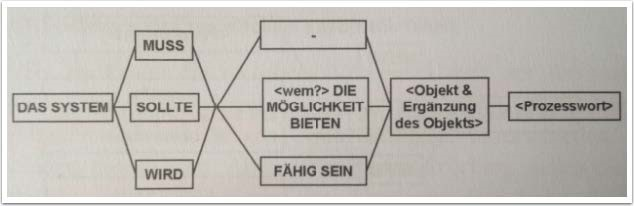
\includegraphics{images/basis-schablone.jpg}
\caption[Basis Schablone \emph{Quelle Rupp}]{Basis Schablone
\emph{Quelle Rupp}\footnotemark{}}
\end{figure}
\footnotetext{Rupp Bilder sind aus dem Buch Basiswissen Requirements
  Engineering \autocite{rupp}}

\begin{figure}[htbp]
\centering
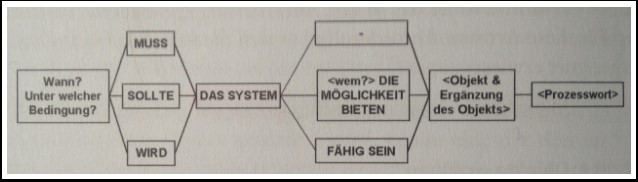
\includegraphics{images/erweiterte-schablone.jpg}
\caption[Erweiterte Schablone \emph{Quelle Rupp}]{Erweiterte Schablone
\emph{Quelle Rupp}\footnotemark{}}
\end{figure}
\footnotetext{Rupp Bilder sind aus dem Buch Basiswissen Requirements
  Engineering \autocite{rupp}}

\newpage

\section{Funktionale Anforderungen}\label{funktionale-anforderungen}

Die funktionalen Anforderungen legen die Funktionen des
Authentifizierungsschnittstellen-Service fest. Die Wünsche des
Arbeitgebers aus sind als Anforderungen umformuliert. Die funktionalen
Anforderungen dienen als Grundlage für die Testfälle. Die Testfälle
wiederum, bringen den Beweis dar, dass alle gewünschten Funktionen
implementiert wurden.

Funktionale Anforderungen werden als FREQ-\emph{Identifikation}
bezeichnet

\subsection{FREQ-111 Programmierer
Registration}\label{freq-111-programmierer-registration}

\begin{longtable}[c]{@{}ll@{}}
\toprule
\begin{minipage}[t]{0.20\columnwidth}\raggedright\strut
\textbf{UC-Referenz}
\strut\end{minipage} &
\begin{minipage}[t]{0.74\columnwidth}\raggedright\strut
UC-11
\strut\end{minipage}\tabularnewline
\begin{minipage}[t]{0.20\columnwidth}\raggedright\strut
\textbf{Beschreibung}
\strut\end{minipage} &
\begin{minipage}[t]{0.74\columnwidth}\raggedright\strut
Ein Programmierer kann sich an der
Authentifizierungsschnittstellen-Service registrieren.
\strut\end{minipage}\tabularnewline
\begin{minipage}[t]{0.20\columnwidth}\raggedright\strut
\textbf{Techn. Risiko}
\strut\end{minipage} &
\begin{minipage}[t]{0.74\columnwidth}\raggedright\strut
Niedrig
\strut\end{minipage}\tabularnewline
\begin{minipage}[t]{0.20\columnwidth}\raggedright\strut
\textbf{Business Value}
\strut\end{minipage} &
\begin{minipage}[t]{0.74\columnwidth}\raggedright\strut
Hoch
\strut\end{minipage}\tabularnewline
\bottomrule
\end{longtable}

\subsection{FREQ-112 Programmierer
Login}\label{freq-112-programmierer-login}

\begin{longtable}[c]{@{}ll@{}}
\toprule
\begin{minipage}[t]{0.20\columnwidth}\raggedright\strut
\textbf{UC-Referenz}
\strut\end{minipage} &
\begin{minipage}[t]{0.74\columnwidth}\raggedright\strut
UC-12
\strut\end{minipage}\tabularnewline
\begin{minipage}[t]{0.20\columnwidth}\raggedright\strut
\textbf{Beschreibung}
\strut\end{minipage} &
\begin{minipage}[t]{0.74\columnwidth}\raggedright\strut
Ein Programmierer muss sich an der
Authentifizierungsschnittstellen-Service mittels E-Mail und Passwort
anmelden.
\strut\end{minipage}\tabularnewline
\begin{minipage}[t]{0.20\columnwidth}\raggedright\strut
\textbf{Techn. Risiko}
\strut\end{minipage} &
\begin{minipage}[t]{0.74\columnwidth}\raggedright\strut
Niedrig
\strut\end{minipage}\tabularnewline
\begin{minipage}[t]{0.20\columnwidth}\raggedright\strut
\textbf{Business Value}
\strut\end{minipage} &
\begin{minipage}[t]{0.74\columnwidth}\raggedright\strut
Hoch
\strut\end{minipage}\tabularnewline
\bottomrule
\end{longtable}

\subsection{FREQ-113 Programmierer Passwort
vergessen}\label{freq-113-programmierer-passwort-vergessen}

\begin{longtable}[c]{@{}ll@{}}
\toprule
\begin{minipage}[t]{0.20\columnwidth}\raggedright\strut
\textbf{UC-Referenz}
\strut\end{minipage} &
\begin{minipage}[t]{0.74\columnwidth}\raggedright\strut
UC-11, UC-12
\strut\end{minipage}\tabularnewline
\begin{minipage}[t]{0.20\columnwidth}\raggedright\strut
\textbf{Beschreibung}
\strut\end{minipage} &
\begin{minipage}[t]{0.74\columnwidth}\raggedright\strut
Ein Programmierer kann ein Passwort per E-Mail anfordern.
\strut\end{minipage}\tabularnewline
\begin{minipage}[t]{0.20\columnwidth}\raggedright\strut
\textbf{Techn. Risiko}
\strut\end{minipage} &
\begin{minipage}[t]{0.74\columnwidth}\raggedright\strut
Niedrig
\strut\end{minipage}\tabularnewline
\begin{minipage}[t]{0.20\columnwidth}\raggedright\strut
\textbf{Business Value}
\strut\end{minipage} &
\begin{minipage}[t]{0.74\columnwidth}\raggedright\strut
Hoch
\strut\end{minipage}\tabularnewline
\bottomrule
\end{longtable}

\subsection{FREQ-114 Programmierer Passwort
ändern}\label{freq-114-programmierer-passwort-uxe4ndern}

\begin{longtable}[c]{@{}ll@{}}
\toprule
\begin{minipage}[t]{0.20\columnwidth}\raggedright\strut
\textbf{UC-Referenz}
\strut\end{minipage} &
\begin{minipage}[t]{0.74\columnwidth}\raggedright\strut
UC-11, UC-12
\strut\end{minipage}\tabularnewline
\begin{minipage}[t]{0.20\columnwidth}\raggedright\strut
\textbf{Beschreibung}
\strut\end{minipage} &
\begin{minipage}[t]{0.74\columnwidth}\raggedright\strut
Ein Programmierer kann sein Passwort ändern. Dafür muss der
Programmierer das alte und neue Passwort angeben.
\strut\end{minipage}\tabularnewline
\begin{minipage}[t]{0.20\columnwidth}\raggedright\strut
\textbf{Techn. Risiko}
\strut\end{minipage} &
\begin{minipage}[t]{0.74\columnwidth}\raggedright\strut
Niedrig
\strut\end{minipage}\tabularnewline
\begin{minipage}[t]{0.20\columnwidth}\raggedright\strut
\textbf{Business Value}
\strut\end{minipage} &
\begin{minipage}[t]{0.74\columnwidth}\raggedright\strut
Hoch
\strut\end{minipage}\tabularnewline
\bottomrule
\end{longtable}

\subsection{FREQ-211 Konfigurieren einer neuen Social-Media Modul
Authentifizierungsvorgang}\label{freq-211-konfigurieren-einer-neuen-social-media-modul-authentifizierungsvorgang}

\begin{longtable}[c]{@{}ll@{}}
\toprule
\begin{minipage}[t]{0.20\columnwidth}\raggedright\strut
\textbf{UC-Referenz}
\strut\end{minipage} &
\begin{minipage}[t]{0.74\columnwidth}\raggedright\strut
UC-21
\strut\end{minipage}\tabularnewline
\begin{minipage}[t]{0.20\columnwidth}\raggedright\strut
\textbf{Beschreibung}
\strut\end{minipage} &
\begin{minipage}[t]{0.74\columnwidth}\raggedright\strut
Ein Programmierer kann ein neuer Authentifizierungsvoragn für sein neus
Social-Media Modul erfassen.
\strut\end{minipage}\tabularnewline
\begin{minipage}[t]{0.20\columnwidth}\raggedright\strut
\textbf{Techn. Risiko}
\strut\end{minipage} &
\begin{minipage}[t]{0.74\columnwidth}\raggedright\strut
Niedrig
\strut\end{minipage}\tabularnewline
\begin{minipage}[t]{0.20\columnwidth}\raggedright\strut
\textbf{Business Value}
\strut\end{minipage} &
\begin{minipage}[t]{0.74\columnwidth}\raggedright\strut
Sehr Hoch
\strut\end{minipage}\tabularnewline
\bottomrule
\end{longtable}

\subsection{FREQ-214 Studien Ergebnis zur Konfiguration
nutzten}\label{freq-214-studien-ergebnis-zur-konfiguration-nutzten}

\begin{longtable}[c]{@{}ll@{}}
\toprule
\begin{minipage}[t]{0.20\columnwidth}\raggedright\strut
\textbf{UC-Referenz}
\strut\end{minipage} &
\begin{minipage}[t]{0.74\columnwidth}\raggedright\strut
UC-21
\strut\end{minipage}\tabularnewline
\begin{minipage}[t]{0.20\columnwidth}\raggedright\strut
\textbf{Beschreibung}
\strut\end{minipage} &
\begin{minipage}[t]{0.74\columnwidth}\raggedright\strut
Ein Programmierer kann zur Konfiguration des Authentifizierungsvorangs
die Studien-Ergebnisse visualisiert nutzen
\strut\end{minipage}\tabularnewline
\begin{minipage}[t]{0.20\columnwidth}\raggedright\strut
\textbf{Techn. Risiko}
\strut\end{minipage} &
\begin{minipage}[t]{0.74\columnwidth}\raggedright\strut
Niedrig
\strut\end{minipage}\tabularnewline
\begin{minipage}[t]{0.20\columnwidth}\raggedright\strut
\textbf{Business Value}
\strut\end{minipage} &
\begin{minipage}[t]{0.74\columnwidth}\raggedright\strut
Mittel
\strut\end{minipage}\tabularnewline
\bottomrule
\end{longtable}

\subsection{FREQ-214 Anpassen eines
Authentifizierungsvorgangs}\label{freq-214-anpassen-eines-authentifizierungsvorgangs}

\begin{longtable}[c]{@{}ll@{}}
\toprule
\begin{minipage}[t]{0.20\columnwidth}\raggedright\strut
\textbf{UC-Referenz}
\strut\end{minipage} &
\begin{minipage}[t]{0.74\columnwidth}\raggedright\strut
UC-21
\strut\end{minipage}\tabularnewline
\begin{minipage}[t]{0.20\columnwidth}\raggedright\strut
\textbf{Beschreibung}
\strut\end{minipage} &
\begin{minipage}[t]{0.74\columnwidth}\raggedright\strut
Ein Programmierer kann ein neues Social-Media Modul erfassen
\strut\end{minipage}\tabularnewline
\begin{minipage}[t]{0.20\columnwidth}\raggedright\strut
\textbf{Techn. Risiko}
\strut\end{minipage} &
\begin{minipage}[t]{0.74\columnwidth}\raggedright\strut
Hoch
\strut\end{minipage}\tabularnewline
\begin{minipage}[t]{0.20\columnwidth}\raggedright\strut
\textbf{Business Value}
\strut\end{minipage} &
\begin{minipage}[t]{0.74\columnwidth}\raggedright\strut
Mittel
\strut\end{minipage}\tabularnewline
\bottomrule
\end{longtable}

\subsection{FREQ-215 Authentifizerungs-Stufe
auswählen}\label{freq-215-authentifizerungs-stufe-auswuxe4hlen}

\begin{longtable}[c]{@{}ll@{}}
\toprule
\begin{minipage}[t]{0.20\columnwidth}\raggedright\strut
\textbf{UC-Referenz}
\strut\end{minipage} &
\begin{minipage}[t]{0.74\columnwidth}\raggedright\strut
UC-21
\strut\end{minipage}\tabularnewline
\begin{minipage}[t]{0.20\columnwidth}\raggedright\strut
\textbf{Beschreibung}
\strut\end{minipage} &
\begin{minipage}[t]{0.74\columnwidth}\raggedright\strut
Ein Programmierer muss eine Authentifizerungs-Stufe für den
Authentifizierungsvorgangs auswählen
\strut\end{minipage}\tabularnewline
\begin{minipage}[t]{0.20\columnwidth}\raggedright\strut
\textbf{Techn. Risiko}
\strut\end{minipage} &
\begin{minipage}[t]{0.74\columnwidth}\raggedright\strut
Niederig
\strut\end{minipage}\tabularnewline
\begin{minipage}[t]{0.20\columnwidth}\raggedright\strut
\textbf{Business Value}
\strut\end{minipage} &
\begin{minipage}[t]{0.74\columnwidth}\raggedright\strut
Hoch
\strut\end{minipage}\tabularnewline
\bottomrule
\end{longtable}

\subsection{FREQ-251 Generierung von Code für einbinden in vorhandenes
System}\label{freq-251-generierung-von-code-fuxfcr-einbinden-in-vorhandenes-system}

\begin{longtable}[c]{@{}ll@{}}
\toprule
\begin{minipage}[t]{0.20\columnwidth}\raggedright\strut
\textbf{UC-Referenz}
\strut\end{minipage} &
\begin{minipage}[t]{0.74\columnwidth}\raggedright\strut
UC-25
\strut\end{minipage}\tabularnewline
\begin{minipage}[t]{0.20\columnwidth}\raggedright\strut
\textbf{Beschreibung}
\strut\end{minipage} &
\begin{minipage}[t]{0.74\columnwidth}\raggedright\strut
Ein Programmierer kann einen Code generieren lassen. Dieser Code soll
ihm die Integration in sein System vereinfachen
\strut\end{minipage}\tabularnewline
\begin{minipage}[t]{0.20\columnwidth}\raggedright\strut
\textbf{Techn. Risiko}
\strut\end{minipage} &
\begin{minipage}[t]{0.74\columnwidth}\raggedright\strut
Sehr Hoch
\strut\end{minipage}\tabularnewline
\begin{minipage}[t]{0.20\columnwidth}\raggedright\strut
\textbf{Business Value}
\strut\end{minipage} &
\begin{minipage}[t]{0.74\columnwidth}\raggedright\strut
Hoch
\strut\end{minipage}\tabularnewline
\bottomrule
\end{longtable}

\subsection{FREQ-311 Authentifizieren}\label{freq-311-authentifizieren}

\begin{longtable}[c]{@{}ll@{}}
\toprule
\begin{minipage}[t]{0.20\columnwidth}\raggedright\strut
\textbf{UC-Referenz}
\strut\end{minipage} &
\begin{minipage}[t]{0.74\columnwidth}\raggedright\strut
UC-31
\strut\end{minipage}\tabularnewline
\begin{minipage}[t]{0.20\columnwidth}\raggedright\strut
\textbf{Beschreibung}
\strut\end{minipage} &
\begin{minipage}[t]{0.74\columnwidth}\raggedright\strut
Ein User kann isch über den Authentifizierungsschnittstellen-Service
authentifizieren um am Social-Media Modul teilzunehmen. Der
Authentifizierungsschnittstellen-Service authentifiziert oder lehnt den
User ab.
\strut\end{minipage}\tabularnewline
\begin{minipage}[t]{0.20\columnwidth}\raggedright\strut
\textbf{Techn. Risiko}
\strut\end{minipage} &
\begin{minipage}[t]{0.74\columnwidth}\raggedright\strut
Mittel
\strut\end{minipage}\tabularnewline
\begin{minipage}[t]{0.20\columnwidth}\raggedright\strut
\textbf{Business Value}
\strut\end{minipage} &
\begin{minipage}[t]{0.74\columnwidth}\raggedright\strut
Sehr Hoch
\strut\end{minipage}\tabularnewline
\bottomrule
\end{longtable}

\subsection{FREQ-411 Report
generieren}\label{freq-411-report-generieren}

\begin{longtable}[c]{@{}ll@{}}
\toprule
\begin{minipage}[t]{0.20\columnwidth}\raggedright\strut
\textbf{UC-Referenz}
\strut\end{minipage} &
\begin{minipage}[t]{0.74\columnwidth}\raggedright\strut
UC-41
\strut\end{minipage}\tabularnewline
\begin{minipage}[t]{0.20\columnwidth}\raggedright\strut
\textbf{Beschreibung}
\strut\end{minipage} &
\begin{minipage}[t]{0.74\columnwidth}\raggedright\strut
Der Programmierer kann ein Report generieren. Der Report soll die
Verwendung übersichtlich darstellen.
\strut\end{minipage}\tabularnewline
\begin{minipage}[t]{0.20\columnwidth}\raggedright\strut
\textbf{Techn. Risiko}
\strut\end{minipage} &
\begin{minipage}[t]{0.74\columnwidth}\raggedright\strut
Mittel
\strut\end{minipage}\tabularnewline
\begin{minipage}[t]{0.20\columnwidth}\raggedright\strut
\textbf{Business Value}
\strut\end{minipage} &
\begin{minipage}[t]{0.74\columnwidth}\raggedright\strut
Sehr Hoch
\strut\end{minipage}\tabularnewline
\bottomrule
\end{longtable}

\newpage

\section{Nicht Funktionale
Anforderungen}\label{nicht-funktionale-anforderungen}

Nicht Funktionale Anforderungen werden als FREQ-\emph{Identifikation}
bezeichnet.

\subsection{NFREQ-110
Betriebsystemunabhängigkeit}\label{nfreq-110-betriebsystemunabhuxe4ngigkeit}

\begin{longtable}[c]{@{}ll@{}}
\toprule
\begin{minipage}[t]{0.20\columnwidth}\raggedright\strut
\textbf{UC-Referenz}
\strut\end{minipage} &
\begin{minipage}[t]{0.74\columnwidth}\raggedright\strut
Alle
\strut\end{minipage}\tabularnewline
\begin{minipage}[t]{0.20\columnwidth}\raggedright\strut
\textbf{Beschreibung}
\strut\end{minipage} &
\begin{minipage}[t]{0.74\columnwidth}\raggedright\strut
Der Authentifizierungsschnittstellen-Service muss auf allen bekannten
Betriebsystemen mit HTML5 und javascritfähigen Browser vewerdent werden
können.
\strut\end{minipage}\tabularnewline
\begin{minipage}[t]{0.20\columnwidth}\raggedright\strut
\textbf{Techn. Risiko}
\strut\end{minipage} &
\begin{minipage}[t]{0.74\columnwidth}\raggedright\strut
Mittel
\strut\end{minipage}\tabularnewline
\begin{minipage}[t]{0.20\columnwidth}\raggedright\strut
\textbf{Business Value}
\strut\end{minipage} &
\begin{minipage}[t]{0.74\columnwidth}\raggedright\strut
Sehr Hoch
\strut\end{minipage}\tabularnewline
\bottomrule
\end{longtable}

\subsection{NFREQ-115 Wartbarkeit}\label{nfreq-115-wartbarkeit}

\begin{longtable}[c]{@{}ll@{}}
\toprule
\begin{minipage}[t]{0.20\columnwidth}\raggedright\strut
\textbf{UC-Referenz}
\strut\end{minipage} &
\begin{minipage}[t]{0.74\columnwidth}\raggedright\strut
UC-51
\strut\end{minipage}\tabularnewline
\begin{minipage}[t]{0.20\columnwidth}\raggedright\strut
\textbf{Beschreibung}
\strut\end{minipage} &
\begin{minipage}[t]{0.74\columnwidth}\raggedright\strut
Die Wartbarkeit des sSystems soll sichergestellt werden
\strut\end{minipage}\tabularnewline
\begin{minipage}[t]{0.20\columnwidth}\raggedright\strut
\textbf{Techn. Risiko}
\strut\end{minipage} &
\begin{minipage}[t]{0.74\columnwidth}\raggedright\strut
Mittel
\strut\end{minipage}\tabularnewline
\begin{minipage}[t]{0.20\columnwidth}\raggedright\strut
\textbf{Business Value}
\strut\end{minipage} &
\begin{minipage}[t]{0.74\columnwidth}\raggedright\strut
Mittel
\strut\end{minipage}\tabularnewline
\bottomrule
\end{longtable}

\subsection{NFREQ-120 Einfache
Integration}\label{nfreq-120-einfache-integration}

\begin{longtable}[c]{@{}ll@{}}
\toprule
\begin{minipage}[t]{0.20\columnwidth}\raggedright\strut
\textbf{UC-Referenz}
\strut\end{minipage} &
\begin{minipage}[t]{0.74\columnwidth}\raggedright\strut
UC-25, UC-21, UC22
\strut\end{minipage}\tabularnewline
\begin{minipage}[t]{0.20\columnwidth}\raggedright\strut
\textbf{Beschreibung}
\strut\end{minipage} &
\begin{minipage}[t]{0.74\columnwidth}\raggedright\strut
Der Authentifizierungsschnittstellen-Service soll einfach im vorhandenen
System eingebunden werden können.
\strut\end{minipage}\tabularnewline
\begin{minipage}[t]{0.20\columnwidth}\raggedright\strut
\textbf{Techn. Risiko}
\strut\end{minipage} &
\begin{minipage}[t]{0.74\columnwidth}\raggedright\strut
Sehr hoch
\strut\end{minipage}\tabularnewline
\begin{minipage}[t]{0.20\columnwidth}\raggedright\strut
\textbf{Business Value}
\strut\end{minipage} &
\begin{minipage}[t]{0.74\columnwidth}\raggedright\strut
Mittel
\strut\end{minipage}\tabularnewline
\bottomrule
\end{longtable}

\subsection{NFREQ-120 Performance}\label{nfreq-120-performance}

\begin{longtable}[c]{@{}ll@{}}
\toprule
\begin{minipage}[t]{0.20\columnwidth}\raggedright\strut
\textbf{UC-Referenz}
\strut\end{minipage} &
\begin{minipage}[t]{0.74\columnwidth}\raggedright\strut
UC-31
\strut\end{minipage}\tabularnewline
\begin{minipage}[t]{0.20\columnwidth}\raggedright\strut
\textbf{Beschreibung}
\strut\end{minipage} &
\begin{minipage}[t]{0.74\columnwidth}\raggedright\strut
Das System soll insbesondere an der Stelle der Authentifzierung
Performant sein.
\strut\end{minipage}\tabularnewline
\begin{minipage}[t]{0.20\columnwidth}\raggedright\strut
\textbf{Techn. Risiko}
\strut\end{minipage} &
\begin{minipage}[t]{0.74\columnwidth}\raggedright\strut
Sehr hoch
\strut\end{minipage}\tabularnewline
\begin{minipage}[t]{0.20\columnwidth}\raggedright\strut
\textbf{Business Value}
\strut\end{minipage} &
\begin{minipage}[t]{0.74\columnwidth}\raggedright\strut
Mittel
\strut\end{minipage}\tabularnewline
\bottomrule
\end{longtable}

\subsection{NFREQ-120 Hohe
Verfügbarkeit}\label{nfreq-120-hohe-verfuxfcgbarkeit}

\begin{longtable}[c]{@{}ll@{}}
\toprule
\begin{minipage}[t]{0.20\columnwidth}\raggedright\strut
\textbf{UC-Referenz}
\strut\end{minipage} &
\begin{minipage}[t]{0.74\columnwidth}\raggedright\strut
UC-25, UC-21, UC22
\strut\end{minipage}\tabularnewline
\begin{minipage}[t]{0.20\columnwidth}\raggedright\strut
\textbf{Beschreibung}
\strut\end{minipage} &
\begin{minipage}[t]{0.74\columnwidth}\raggedright\strut
Der Authentifizierungsschnittstellen-Service soll eine Hohe
Verfügbarkeit von 99.9\%
\strut\end{minipage}\tabularnewline
\begin{minipage}[t]{0.20\columnwidth}\raggedright\strut
\textbf{Techn. Risiko}
\strut\end{minipage} &
\begin{minipage}[t]{0.74\columnwidth}\raggedright\strut
Hoch
\strut\end{minipage}\tabularnewline
\begin{minipage}[t]{0.20\columnwidth}\raggedright\strut
\textbf{Business Value}
\strut\end{minipage} &
\begin{minipage}[t]{0.74\columnwidth}\raggedright\strut
Mittel
\strut\end{minipage}\tabularnewline
\bottomrule
\end{longtable}

\newpage

\newpage

\section{Risiken}\label{risiken}

Nachfolgend sind die im Gespräch mit dem Auftraggeber gefundenen
Riskiken bezüglich der Bachelorarbeit, sowie deren Auswirkungen,
aufgeführt.

\subsection{R-01 Akzeptanz}\label{r-01-akzeptanz}

Programmierer und insbesondere auch User, welche den
Authentifizierungsschnittstellen-Service verwenden soll, sind völlig
unterschiedlich. Deren unterschiedliche Ansprüche machen es schwierig,
eine Lösung zu entwickeln welchen Akteuren gerecht wird.

Da der Auftraggeber sowohl die Zielgruppe Programmierer wie auch User
kenn, kann er hier gezielt Feedback geben.

Die Auswirkung bei Eintritt dieses Risikos ist im Rahmen der
Bachelorarbeit gering, da der Erfolg der Arbeit nicht von der
tatsächlichen Verwendung im produktiven Umfeld abhängt.

\subsection{R-02 Kosten}\label{r-02-kosten}

Da es sich bei diesem Projekt um eine Bachelorarbeit handelt, besteht
kein Personalkostenrisiko. Kostenpflichtige Produkte Dritter werden
nicht verwendet. Einzig der Betrieb/Hosting der Bachelorarbeit
verursacht Kosten. Das Kostenrisiko kann dank fixen Leistungsparameter
auf ein Minimum reduziert werden.

\subsection{R-03 Überkomplexität}\label{r-03-uxfcberkomplexituxe4t}

Es besteht die Möglichkeit, dass die Komplexität des zu entwickelnden
Systems viel höher ist, als angenommen. Da die Komplexität nur zu einem
gewissen Grad durch Architekturentscheide beeinflusst werden kann, muss
besonderes Augenmerk auf dieses Risiko gelegt werden.

Dieses Risiko wird mit hoher Wahrscheinlichkeit eintreten.

Die Auswirkung bei Eintritt dieses Risikos ist, dass nicht der gesamte
Umfang der Bachelorarbeit erarbeitet werden kann, weil zur Lösung der
Komplexitätsprobleme zusätzliche Zeit benötigt wird.

\subsection{R-04
Systemumfeldänderungen}\label{r-04-systemumfelduxe4nderungen}

Umsysteme könnten während der Projektphase dieser Bachelorarbeit
massgeblich verändert werden.

Dieses Risiko wird mit sehr geringer Wahrscheinlichkeit eintreten.

Die Auswirkung bei Eintritt dieses Risikos kann nicht abgeschätzt
werden. Situativ muss dieses Risiko behandelt werden.

\subsection{R-05 Schlechte/Unzureichende
Framework}\label{r-05-schlechteunzureichende-framework}

Die Bachelorarbeit wird basierend auf verschiedenen Frameworks
umgesetzt. Das Risiko, dass Frameworks nicht wie beschrieben
funktionieren, schlecht dokumtiert oder instabil sind besteht.

Dieses Risiko wird mit mittlerer Wahrscheinlichkeit eintreten Als
Auswirkungen dieses Risikos sind Wechsel des Frameworks oder gar
manuelle Entwicklungen und daraus zusätzliche nicht einschätzbare
Aufwendungen nötig.

\subsection{R-06 Termineinhaltung}\label{r-06-termineinhaltung}

Der fixe Abgabetermin der Semesterarbeit gilt es einzuhalten. Das Risiko
das die Arbeit verspätet abgegeben wird besteht.

Dieses Risiko wird mit geringer Wahrscheinlichkeit eintreten. Die
Auswirkung bei Eintritt dieses Risikos ist das nicht Bestehen der
Arbeit.

\subsection{R-07 Auslastung}\label{r-07-auslastung}

Das Projekt wird durch einen Mitarbeiter getragen. Dieser ist sowohl im
Beruf wie auch privat stark ausgelastet. Der hohe schulische Aufwand
kann beeinflusst werden. Mit zusätzliche Ausfälle durch Krankheit oder
nicht vorhersehbaren Vorfällen muss gerechnet werden.

Das Risiko wird mit mittlerer Wahrscheinlichkeit eintreten. Die
Auswirkungen bei Eintritt dieses Risikos werden sich in der Qualität und
Quantität der Arbeit wiederspiegeln.

\newpage

\subsection{Risikomatrix}\label{risikomatrix}

\begin{figure}[htbp]
\centering
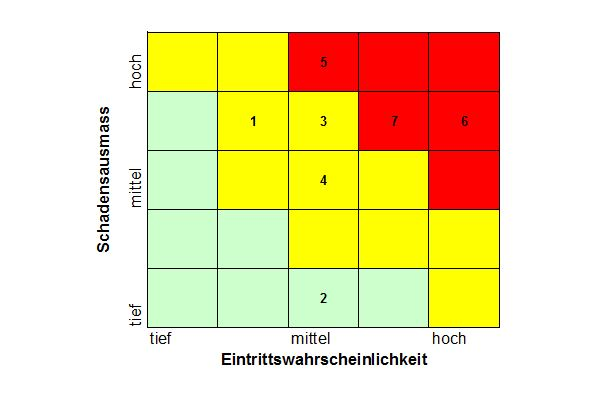
\includegraphics{images/excel-statistik/risikomatrix.JPG}
\caption[Risikomatrix ]{Risikomatrix \footnotemark{}}
\end{figure}
\footnotetext{Die Risikomatrix wurde basierend auf der Excel-Vorlage der
  Stadtpolizei Zürich Abteilung Informatik entworfen}

Rot: Massnahmen erforderlich

Gelb: Risiken beobachten

Grün: Keine Massnahmen erforderlich

1 Akzeptanz

2 Kosten

3 Überkomplexität

4 Systemumfeldänderungen

5 Schlechte/Unzureichende Frameworks

6 Termineinhaltung

7 Auslastung

\subsection{Massnahmen}\label{massnahmen}

Um das Zusammenspiel der verschiedenen Technologien und die daraus
resultierende Komplexität einschätzen zu können wird vor Projektbeginn
ein Prototyp mittels Durchstich durch alle Technologien erstellt. Danach
kann die Komplexität im Zusammenspiel der Technologie eingeschätzt und
bei Bedarf eine Technologie durch eine andere Ersetzt werden. So kann
das Risiko 3 Überkomplexität und Risiko 5 Schlechte/Unzureichende
Frameworks minimiert werden.

Das Projekt ist über eine Anzahl von Feiertagen gelegt, welche gebraucht
werden könnten. Zusätzlich wurden vom Studenten eine Arbeitswoche Ferien
genommen, welche im Notfall auch für die Arbeit verwendet werden könnte.
Durch diese Massnahmen sollte das Risiko 6 Termineinhaltung minimal
bleiben. Das Risiko 7 Auslastung kann nicht direkt vermindert werden.
Die Aktivitäten im Bereich der freiwilligen Arbeit wurde auf ein Minimum
reduziert. Für die restliche freiwilige Arbeit wurde mit Freunden ein
Nofallszenario entwickelt, so kann der Student bei Bedarf seine
freiwillige Arbeit durch andere Personen übernehmen lassen. Der Kontakt
mit dem mit Arbeitgeber wird intensiv gepflegt um, so bei Bedarf die
Arbeitsbelastung zu vermindern. Die Massnahmen welche für Risiko 6
ergriffen wurden entschärfen auch Risiko 7.

\chapter{Konzept}\label{konzept}

In diesem Kapitel soll ein System für den Authentifizierungsservice
entworfen werden. Das System soll den Anforderungen, welche im
vorherigen Kapitel definiert wurden, entsprechen.

Um die Komponenten unabhängig von einander zu entwickeln, wird bei der
Entwicklung der Architektur des Authtenifizierungsservice darauf geachte
möglichst gerine Kopplung aufzuweisen.

\section{Architektur}\label{architektur}

Der Authtentifizierungsservice besteht aus drei Hauptkomponenten:
Web-API, Konfigurator und Autorisierung. Die folgende Abbildung zeigt
die Verbindungen der drei Hauptkomponenten im Systemkontext des
Authentifizierungservice auf.

\begin{figure}[htbp]
\centering
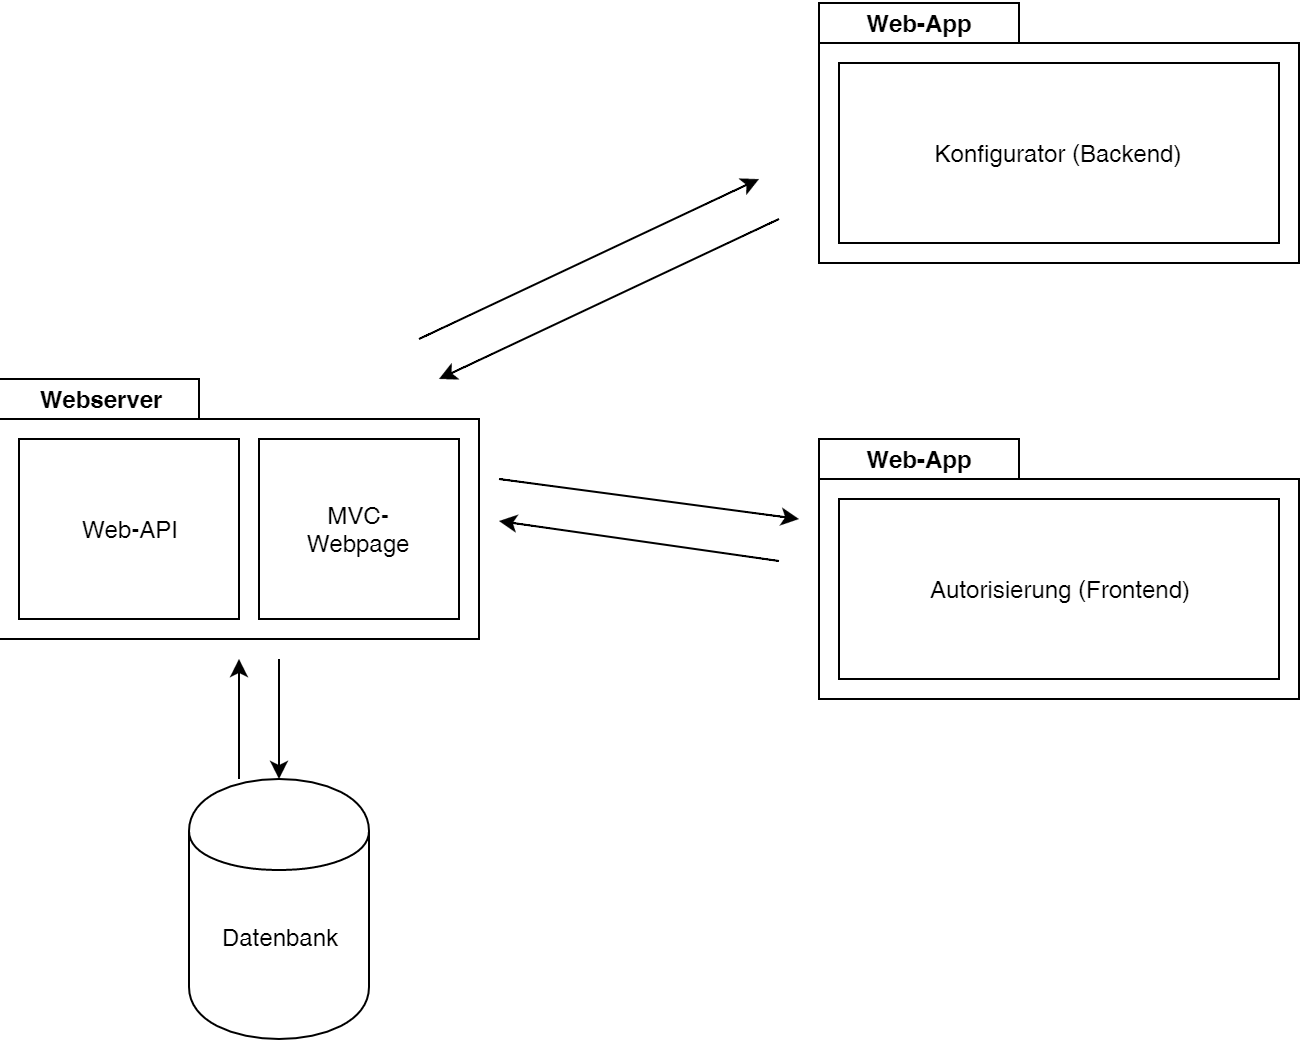
\includegraphics{images/draw_io/BA_KomponentenDiagramm.png}
\caption{Übersicht der Hauptkomponenten}
\end{figure}

\section{Software Design}\label{software-design}

\subsection{Webservice}\label{webservice}

\subsection{}\label{section}

\newpage

\section{Ablauf Authentifizierung}\label{ablauf-authentifizierung}

Der User nimmt an einer Interaktivität eines Anbieters teil. Dabei füllt
er den Wettbewerb, Umfrage aus oder löst die gegebene Aufgabe und sendet
einmal oder mehrmals ein Feedback an die Anbieter Webseite zurück. Nach
Abschluss der Interaktivität, werden die Datengespeichert und mit der
daraus resultierenden eindeutigen Identität des Feedbacks wird die
Authentifizierung gestartet. Das vom Programmierer definierte
Authentifizierungsverfahren wird durchgeführt um Identität im
gewünschten Masse sicher zustellen. User und das Anbieter System werden
über erfolgreiche Authentifizierung informiert. Nach Möglichkeit wird
auch eine fehlerhafte Authentifizierung mitgeteilt.

\begin{figure}[htbp]
\centering
\includegraphics{images/draw_io/BA_AutorisationOverview.png}
\caption{Aufbau Inhalt im Card-Design}
\end{figure}

\section{Domänenmodel
Differenziert}\label{domuxe4nenmodel-differenziert}

Ein differenziertes Domänemodel oder auch Domänenmodel Basis Level
genannt, erlaubt eine vereinfachte Kommunikation zwischen
Kunde/Auftraggeber und Entwicklungsteam/Entwicklungsperson. Die
Denkweise im Model erfordert keine Programmierkenntnisse und fördert die
strukturierte Wiedergabe von Datengefässen. Beim Domänenmodel werden die
Begriffe aus der Domäne des Kunden verwendet und fördern so die
Verständlichkeit auf beiden Seiten.

\begin{figure}[htbp]
\centering
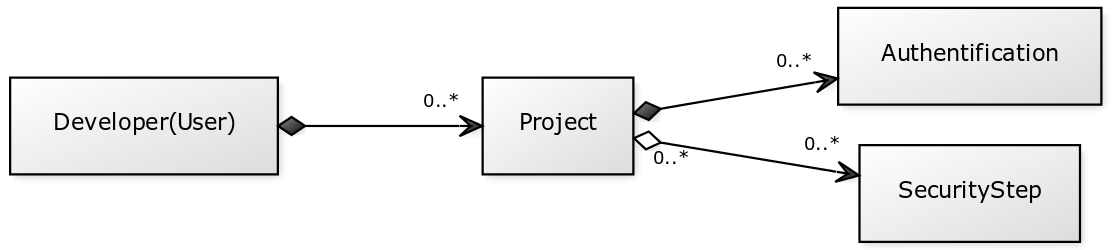
\includegraphics{images/domaenenmodell.png}
\caption{Differenziertes Domänemodel des Authentifizierungservice}
\end{figure}

\newpage

\section{Datenbankdesign}\label{datenbankdesign}

In der Systemarchitektur des Authentifizierungservice stehen Objekte nur
während der Ausführungszeit zur Verfügung. Um sie zu persitieren, werden
sie in einer relationalen Datenbank gespeichert. Die Pradigmen der
Objektorientierten Programmiersprache und der relationalen Datenbank
sind grundlegend verschieden. So kapseln Objekte ihren Zustand und ihr
Verhalten hinter einer Schnittstelle und haben eine eindeutige
Identität. Relationale Datenbanken basieren dagegen auf dem
mathematischen Konzept der relationalen Algebra. Dieser konzeptionelle
Widerspruch wurde in den 1990er Jahren als ``object-relational impedance
mismatch'' bekannt.{[}\^{}the-vietnam-of-computer-science{]} Um diesen
Wiederspruch zu mindern stellt Microsoft das Entity-Framework zur
Verfügung. Das Entity-Framework hat verschiedene Konzeptionelle Ansätze.
Es gilt nun den richtigen Ansatz für den Authenifizierungsservice zu
wählen

\subsection{Database First}\label{database-first}

Beim Database First Ansatz wird zuerst die Datenbank designt. Das
Entity-Framework bildet aus der Datenbank die POCO-Klassen ab. Sollten
Anpassungen an den Entitäten ergeben, werden diese zuerst in der
Datenbank implementiert und daraus werden wiederum neuen POCO-Klassen
generiert.

\subsection{Code First}\label{code-first}

Beim Code First Ansatz werden zuerst die POCO-Klassen erstellt. Das
Entity-Framework bildet aus den POCO-Klassen die Tabellen in der
Datenbank. Alle Anpassungen werden gleich in den POCO-Klassen umgesetzt
und durch das Entity-Framework in der Datenbank geändert erstellt.

\subsection{Entscheidung}\label{entscheidung}

Wenn die POCO-Klassen gleich mehrheitlich für die
Schnittstellendefinition als Parameterdefinition verwendet werden
könnten, fallen Mehraufwendungen für Umwandlungen im Programmcode weg.
Eine Schnittstellendefinition sollte aber nicht willkürlich durch eine
Datenbankänderung beeinflusst werden. Der umgekehrte Fall ist aber
minder wichtig, da die Datenbank nur von der Schnittstelle verwendet
wird. Deshalb wird das Konzept Code First eingesetzt.

\subsection{ERD}\label{erd}

Durch den Codefirst Ansatz werden die Datenbank und alle zugehörigen
Tabellen durch das Entity Framework selbständig generiert
{[}\^{}the-vietnam-of-computer-science{]}:
\autocite{the-vietnam-of-computer-science}

\section{Integration der
Schnittstelle}\label{integration-der-schnittstelle}

Wie in der Anforderungsanalyse und Aufgabenstellung geschrieben, soll
die Schnittstelle möglichst einfach in Bestehende Systeme integriert
werden können. Bevor wir untersuchen wie wir die Integration umsetzten
können, bedarf es die wichtigsten bestehenden Systeme zu kennen um evtl
für diese Systeme eine spezifisch einfach Integration zu entwickeln.

\subsection{Bestehende Systeme für Votings, Wettbewerbe und
Quizes}\label{bestehende-systeme-fuxfcr-votings-wettbewerbe-und-quizes}

Das bestehende Social-Media Modul wird als Teil einer Webseite in einer
Webapplikation geführt. Webapplikation, welche Inhalte verwalten, werden
sinngemäss Content Management Systeme genannt. Die Abkürzung CMS hat
sich im IT-Fachjargon etabliert. Statista.com wertetet mehrmals im Jahr
die Verbreitung der verschiedenen CMS aus \footnote{CMS
  Nutzungsstatistik von statista.com \autocite{statisticinfostatista}}.
Folgend ist die Erhebung aus dem November 2015 abgebildet:

\begin{figure}[htbp]
\centering
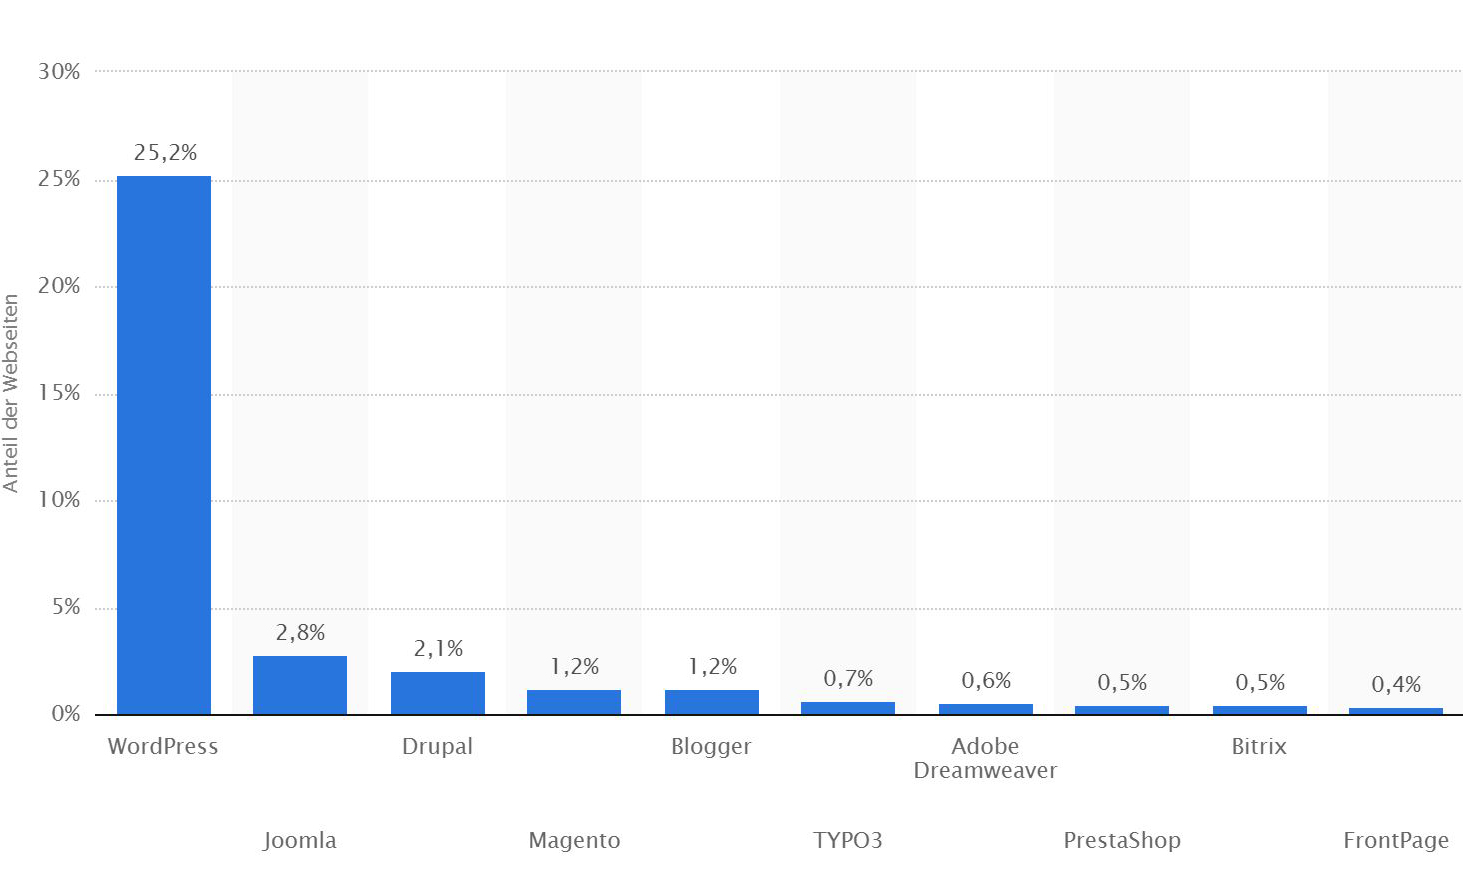
\includegraphics{images/cms_statistik_november2015.JPG}
\caption{Nutzungsanteil CMS weltweit \emph{Quelle:de.statista.com}}
\end{figure}

Die von statista.com veröffentlichten Zahlen wurden mit Werten von
W3techs.com verglichen\footnote{CMS Nutzungsstatistik von w3techs.com
  \autocite{statisticinfow3techs}}. Die Unterschiede sind für unsere
Verwendung minimal und liegen im 10tels Prozentbereich. Da beide
bekannten Statistik unternehmen auf die selben Werte gekommen sind, kann
von einem hohen Warheitsgrad ausgegangen werden. Beim Betrachten der
Statistik fällt auf das Wordpress mit 25,2 mit Abstand am meisten
genutzt wird. Alle dynamischen Webseiten unter den Top 10 basieren auf
Systemen in PHP\footnote{Die Information wurde von den jeweiligen
  Hersteller- bzw. Communitywebseiten bezogen.}. Adobe Dreamviewer und
FrontPage sind keine Systeme welche auf dem Server betrieben werden. Sie
sind Editoren welche auf dem jeweiligen Computer ausgeführt werden und
danach mehrheitlich HTML, CSS und Javascript Code an den Server
ausliefern. Funktionalitäten werden mit den beiden Editoren manuell
geschrieben.

Basierend auf diesen statistischen Erkenntnissen lohnt es sich die
Wordpress Welt kennen zu lernen und recherchieren wie dort eine
Authentifizierungsschnittstelle eingebunden werden könnte.

\subsection{Wordpress PlugIn Hook}\label{wordpress-plugin-hook}

Erweiterungen im Wordpress nennen sich Plugins. Die Plugins können
direkt über das CMS-Backend eingespielt werden. Alternativ können Sie
natürlich manuell installiert werden. Zum Beispiel in dem man ein Plugin
selber Programmiert oder beim Hersteller oder über das
Plugin-Verzeichnis von Wordpress{[}\^{}plugin-verzeichnis{]}
downloadedt. Wordpress sammelt zugleich die aktiven Installationen der
PlugIns (sofern man als Entwickler den Informationsaustausch nicht
unterbindet). Die Gesamtzahl wird im CMS-Backend Wordpress und auf Ihrer
Plugin-Verzeichnis Webseite{[}\^{}plugin-verzeichnis{]} veröffentlicht.
Dank dieser Kennzahl kann nun die meist verbreiteten Plugins
herrausgefunden werden.

Wordpress basiert auf einem sogennanten Hook-System. ``Hook'' eins zu
eins übersetzt bedeutet ``Haken'', ``Aufhänger'' oder ``Greifer''. Ein
Hook ist im Wordpress eine definierte Codestelle bei der man seinen
eigenen Code einhaken kann. Der PlugIn Entwickler definiert diese Hooks
um anderen PlugIns oder Funktionalitäten zu erlauben sein PlugIn zu
erweitern. Auch der Core vom Wordpress enthält solche Hooks. Dadurch
soll verhindert werden, dass PlugIn's oder der Core von Wordpress direkt
umgeschrieben werden muss und dann nicht mehr einfach so unabhängig
upgedatet werden kann. Um unsere Schnittstelle einzubinden, könnten wir
evtuell also solche Hooks verwenden. Dieser ``Hook''/Haken hat
lustigerweise auch einen Haken: Der PlugIn-Entwickler kann selbständig
bestimmen ob und wo er solche Hooks einsetzen will und welche
Möglichkeiten dann zur Verfügung stehen. Kommerzielle PlugIn's verfolgen
vielfach den Weg möglichst verschlossen zu agieren um mögliche
Erweiterungen monetär umzusetzen und so eine Abhängigkeit zu erzeugen.
Diese These gilt es nun zu untersuchen. Dafür wurden verschiedene Social
Plugin's ausgewählt. Die Top 1000 installierten Wordpress PlugIns welche
von der Art Social-Media Modul waren, ein paar Stichproben von
kommerziellen Plugins und Stichproben aus in Beiträgen empfohlenen
PlugIns: \footnote{Das Pluginverzeichnis befindet sich unter
  http://de.wordpress.org/plugins}, \footnote{Envato bietet eine
  Plattform für den Verkauf von Wordpress-Plugin's an
  http://market.envato.com}

\begin{longtable}[c]{@{}llll@{}}
\caption{Recherche PlugIn's}\tabularnewline
\toprule
\begin{minipage}[b]{0.33\columnwidth}\raggedright\strut
\textbf{PlugIn}
\strut\end{minipage} &
\begin{minipage}[b]{0.14\columnwidth}\raggedright\strut
\strut\end{minipage} &
\begin{minipage}[b]{0.14\columnwidth}\raggedright\strut
\strut\end{minipage} &
\begin{minipage}[b]{0.28\columnwidth}\raggedright\strut
\strut\end{minipage}\tabularnewline
\midrule
\endfirsthead
\toprule
\begin{minipage}[b]{0.33\columnwidth}\raggedright\strut
\textbf{PlugIn}
\strut\end{minipage} &
\begin{minipage}[b]{0.14\columnwidth}\raggedright\strut
\strut\end{minipage} &
\begin{minipage}[b]{0.14\columnwidth}\raggedright\strut
\strut\end{minipage} &
\begin{minipage}[b]{0.28\columnwidth}\raggedright\strut
\strut\end{minipage}\tabularnewline
\midrule
\endhead
\begin{minipage}[t]{0.33\columnwidth}\raggedright\strut
\textbf{WP-Polls}
\strut\end{minipage} &
\begin{minipage}[t]{0.14\columnwidth}\raggedright\strut
kostenlos
\strut\end{minipage} &
\begin{minipage}[t]{0.14\columnwidth}\raggedright\strut
100000+
\strut\end{minipage} &
\begin{minipage}[t]{0.28\columnwidth}\raggedright\strut
Über ``wp\_polls\_add\_poll'' könnte man den erstellten Poll
authentfizieren und bei fehlerhafter Authentifizierung löschen
\strut\end{minipage}\tabularnewline
\begin{minipage}[t]{0.33\columnwidth}\raggedright\strut
\_\_Polldaddy Polls \& Ratings\_
\strut\end{minipage} &
\begin{minipage}[t]{0.14\columnwidth}\raggedright\strut
\_ Freemium
\strut\end{minipage} &
\begin{minipage}[t]{0.14\columnwidth}\raggedright\strut
20000+
\strut\end{minipage} &
\begin{minipage}[t]{0.28\columnwidth}\raggedright\strut
-
\strut\end{minipage}\tabularnewline
\begin{minipage}[t]{0.33\columnwidth}\raggedright\strut
\textbf{Wp-Pro-Quiz}
\strut\end{minipage} &
\begin{minipage}[t]{0.14\columnwidth}\raggedright\strut
kostenlos
\strut\end{minipage} &
\begin{minipage}[t]{0.14\columnwidth}\raggedright\strut
20000+
\strut\end{minipage} &
\begin{minipage}[t]{0.28\columnwidth}\raggedright\strut
Hooks vorhanden. Nicht für eine Authentifizierungsschnittstelle zu
gebrauchen.
\strut\end{minipage}\tabularnewline
\begin{minipage}[t]{0.33\columnwidth}\raggedright\strut
\textbf{Responsive Poll}
\strut\end{minipage} &
\begin{minipage}[t]{0.14\columnwidth}\raggedright\strut
15\$
\strut\end{minipage} &
\begin{minipage}[t]{0.14\columnwidth}\raggedright\strut
-
\strut\end{minipage} &
\begin{minipage}[t]{0.28\columnwidth}\raggedright\strut
Keine Hooks. Laut Hersteller sind welche geplant (Zeitpunkt ungewiss)
\strut\end{minipage}\tabularnewline
\begin{minipage}[t]{0.33\columnwidth}\raggedright\strut
\textbf{TotalPoll Pro}
\strut\end{minipage} &
\begin{minipage}[t]{0.14\columnwidth}\raggedright\strut
18\$
\strut\end{minipage} &
\begin{minipage}[t]{0.14\columnwidth}\raggedright\strut
-
\strut\end{minipage} &
\begin{minipage}[t]{0.28\columnwidth}\raggedright\strut
Hooks vorhanden. Ähnlich wie bei WP-Polls könnte man evtl. den
erstellten Datensatz löschen. Jedoch ist dies ohne Kauf nicht
ersichtlich.
\strut\end{minipage}\tabularnewline
\begin{minipage}[t]{0.33\columnwidth}\raggedright\strut
\textbf{Easy Polling}
\strut\end{minipage} &
\begin{minipage}[t]{0.14\columnwidth}\raggedright\strut
15\$
\strut\end{minipage} &
\begin{minipage}[t]{0.14\columnwidth}\raggedright\strut
-
\strut\end{minipage} &
\begin{minipage}[t]{0.28\columnwidth}\raggedright\strut
-
\strut\end{minipage}\tabularnewline
\begin{minipage}[t]{0.33\columnwidth}\raggedright\strut
\textbf{Opinion Stage}
\strut\end{minipage} &
\begin{minipage}[t]{0.14\columnwidth}\raggedright\strut
kostenlos
\strut\end{minipage} &
\begin{minipage}[t]{0.14\columnwidth}\raggedright\strut
10000+
\strut\end{minipage} &
\begin{minipage}[t]{0.28\columnwidth}\raggedright\strut
-
\strut\end{minipage}\tabularnewline
\begin{minipage}[t]{0.33\columnwidth}\raggedright\strut
\textbf{Wedgies}
\strut\end{minipage} &
\begin{minipage}[t]{0.14\columnwidth}\raggedright\strut
Freemium
\strut\end{minipage} &
\begin{minipage}[t]{0.14\columnwidth}\raggedright\strut
800+
\strut\end{minipage} &
\begin{minipage}[t]{0.28\columnwidth}\raggedright\strut
-
\strut\end{minipage}\tabularnewline
\bottomrule
\end{longtable}

Wir haben nun verschiedene Wordpress-Plugin's für Umfragen, Wettbewerbe
\& Abstimmungen auf Hooks untersucht. Alle PlugIn's bieten gar keinen
Hook an oder keinen Hook, welcher unseren Anforderungen einer einfachen
Integration genügt. Die aufgelisteten Plugins bilden eine wesentliche
Verbreitung ab. Selbst wenn wieder erwartet alle nicht untersuchten
Plugin's eine perfekte Hookanbindung liefern würden, hätten wir, mit den
nicht getesteten Plugin's eine zu geringe Verbreitung. Der Ansatz die
Integration per Hooks zu machen muss also fallen gelassen werden.

\newpage

\subsection{Parallellen im ähnliches
Anwendungsfeld}\label{parallellen-im-uxe4hnliches-anwendungsfeld}

Der vertieften Research der letzten Kapitel wird verlassen und es wird
probiert einen anderen Herangehensweise zur Findung der Lösung zu
nehmen: Forscher adaptieren immer wieder erfolgreiche Modelle aus
anderen Bereich in ihr Gebiet. Vielfach wird die Natur als erfolgreiches
Vorlagemodell genommen. Ganz soweit wird hier nicht gegangen.
Payment-Gateways wie der Schweizer Anbieter Datatrans müssen
Webshop-Entwicklern auch eine Möglichkeit bieten das Gateway einfach in
Ihren Webshop einbinden zu können. Auch bei Ihnen steht die Sicherheit
auf der obersten Stufe und eine einfache Integration ist für den Erfolg
trotz internationalem Druck von nöten. Dabei fährt Datatrans eine
Zweiwegstrategie. Sie stellen für bekannte Shopsysteme gleich ganze
PlugIns zur Verfügung\footnote{Übersicht der Web-Shop PlugIn's
  \autocite{datatrans-plugin}}. Auf der anderen Seite bieten Sie
ausführliche beschriebene und einfache Schnittstellen an.

\subsubsection{Datatrans Zahlungsablauf}\label{datatrans-zahlungsablauf}

Um die Gateway-Implementation der Datatrans als Ganzes zu verstehen,
führen wir uns der generellen Ablauf eines Payment Gateways eines
Webshopeinkaufs bei Datatrans vor Augen. Der Ablauf:

\begin{figure}[htbp]
\centering
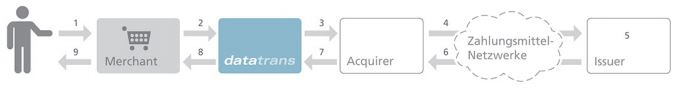
\includegraphics{images/datatrans-autorisierung.JPG}
\caption{Nutzungsanteil Zahlungsablauf Webshop mit Datatrans
\emph{Quelle:datatrans}}
\end{figure}

\begin{enumerate}
\def\labelenumi{\arabic{enumi}.}
\tightlist
\item
  Der Endkunde wählt Produkt aus und schliesst die Bestellung ab
\item
  Der Webshop/Merchant zeigt Zahlungsseite von Datatrans, Karteninhaber
  gibt seine Kartendaten ein. 3.-7.Datatrans autorisiert und verarbeitet
  wennmöglich die Transaktion zum Acquirer.
\item
  Datatrans zeigt den Status dem Kunden an und sendet Status dem
  Merchant zurück.
\item
  Merchant zeigt dem Karteninhaber die Antwortseite (erfolgreich oder
  abgelehnt) \footnote{Für die Bachelorarbeit wurde die V 9.1.13
    verwendet \autocite{datatrans-api}}
\end{enumerate}

\newpage

\subsubsection{Datatrans XML/SOAP API Lightbox
Mode}\label{datatrans-xmlsoap-api-lightbox-mode}

Bei Schritt 2 des Zahlungsablaufs ruft der Webshop das Datatransgateway
auf. Beim ``Lightbox Mode'' wird dabei ein iframe in einem Overlay über
die Webseite gelegt und der Webshop ansich verdunkelt dargestellt.

\begin{figure}[htbp]
\centering
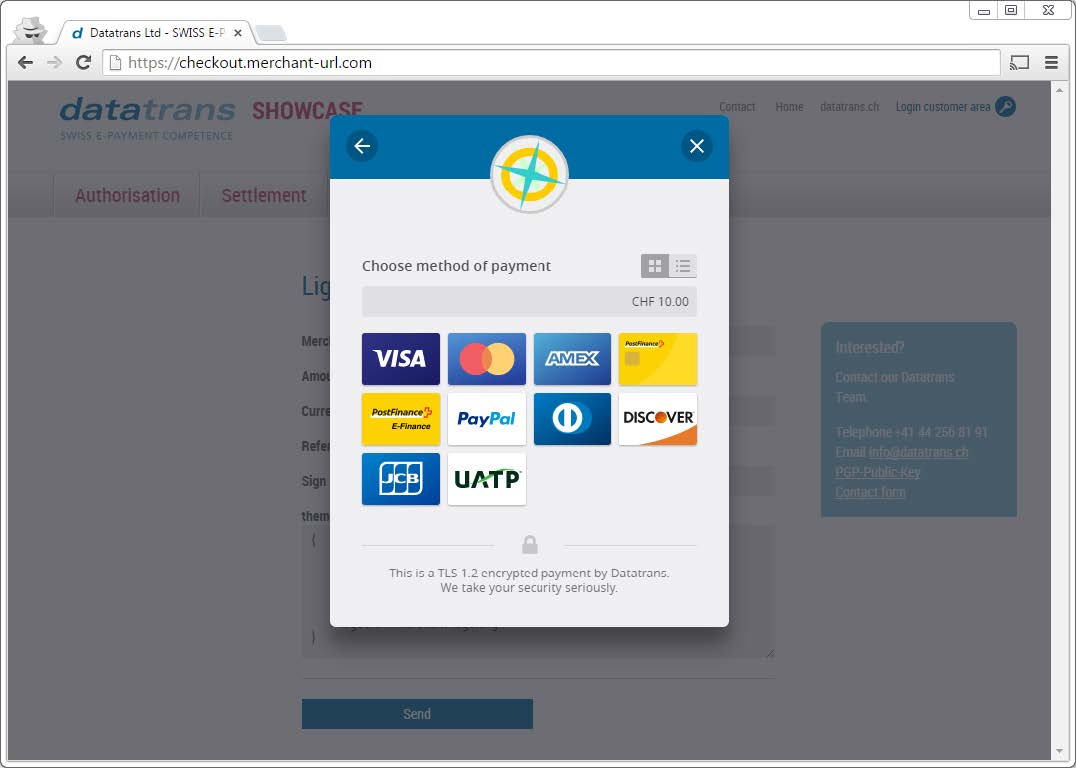
\includegraphics{images/datatrans-lightbox.JPG}
\caption{Datatrans Lightbox Integration \emph{Quelle:datatrans}}
\end{figure}

Das Gateway muss eine minimum an Informationen erhalten, um den
Zahlungsvorgang überhaupt starten zu können. So muss es wissen, wer der
Verchäufer ist. Datatrans regelt dies über eine Merchan-ID. Wie viel
Geld in welcher Währung verkauft werden sollte, muss Datatrans über
amount und currceny mitgeteilt werden. Um dem Shop später mitteilen zu
können, welche Bestellung erfolgreich verarbeitet wurde, braucht es eine
Referenznummer. Die Referenznummer nennt Datatrans singemäss refno. Die
Ganzen Parameter werden optional mit einem sign-Parameter gesichert und
mittels Html-Form dem Javascript übergeben:\footnote{Für die
  Bachelorarbeit wurde die V 9.1.13 verwendet \autocite{datatrans-api}}

\newpage

Implementierungscode der Datatrans:

\begin{verbatim}
<script src="https://code.jquery.com/jquery-1.11.2.min.js"></script>
<script src="https://pilot.datatrans.biz/upp/payment/js/datatrans-1.0.2.js"></script>

    <form id="paymentForm"
         data-merchant-id="1100004624"
         data-amount="1000"
         data-currency="CHF"
         data-refno="123456789"
         data-sign="30916165706580013">
         <button id="paymentButton">Pay</button>
    </form>
    
<script type="text/javascript">
     $("#paymentButton").click(function () {
        Datatrans.startPayment({'form': '#paymentForm'});
     });
</script>
\end{verbatim}

\subsection{Integrationsentscheid}\label{integrationsentscheid}

Die Stragtegie der Paymentintegration von Datatrans soll für den
Authentifizierungservice genutzt werden.

Durch automatisches Öffnen der Lightbox erreicht der Endbenutzer mühelos
den Schritt der Authentifizierung. Die Authentifzierung springt ihm nahe
zu entgegen. Dadurch ist eine Hohe Effiktivität gegeben. Der User bleibt
auf der selben Seite und wird dadurch nicht aus dem Fluss der
Abarbeitung der Interaktivität geworfen. Das Verfahren ist sehr
effizient. Die Javascript und CSS Daten werden beim Laden der
Interaktivität bereits mit geladen. So entsteht eine minimale Wartezeit
beim Einblenden der Lightbox. Dies ist für den User nicht spürbar oder
störend.

Bei der Darstellung der Authentifizierung auf einer einzelnen Seite
müsste das Web-Design des Interaktivitäs-Anbiter adaptiert werden
können. Da die Authentifizierungs-Lightbox auf seiner Seite dargestellt
wird, braucht der Interaktivitäts-Anbieter nicht sein Design mühsam für
eine Authentifizierungsseite zu konfigurieren.

Die Lightbox des Authenifizierungsservice wird mit einer grösseren
Verbreitung einen gewissen Wiedererkennungswert erhalten. So wird die
Lösung als professionelles Produkt wahrgenommen werden. Das Ziel das
Benutzer und Entwickler den Authenifizierungsservice als ein sicheres
und glaubwürdiges Produkt für Interaktivitäten wahrnehmen wird so
versteckt werden.

\subsection{Integrationskonzept}\label{integrationskonzept}

\subsection{Integrationsparameter}\label{integrationsparameter}

\begin{longtable}[c]{@{}lll@{}}
\caption{Parameter Authenifizierungsservice Lightbox}\tabularnewline
\toprule
\begin{minipage}[b]{0.30\columnwidth}\raggedright\strut
\textbf{Feldname}
\strut\end{minipage} &
\begin{minipage}[b]{0.17\columnwidth}\raggedright\strut
\textbf{Wert}
\strut\end{minipage} &
\begin{minipage}[b]{0.43\columnwidth}\raggedright\strut
\textbf{Beschreibung}
\strut\end{minipage}\tabularnewline
\midrule
\endfirsthead
\toprule
\begin{minipage}[b]{0.30\columnwidth}\raggedright\strut
\textbf{Feldname}
\strut\end{minipage} &
\begin{minipage}[b]{0.17\columnwidth}\raggedright\strut
\textbf{Wert}
\strut\end{minipage} &
\begin{minipage}[b]{0.43\columnwidth}\raggedright\strut
\textbf{Beschreibung}
\strut\end{minipage}\tabularnewline
\midrule
\endhead
\begin{minipage}[t]{0.30\columnwidth}\raggedright\strut
\textbf{as\_projectid}
\strut\end{minipage} &
\begin{minipage}[t]{0.17\columnwidth}\raggedright\strut
Integer
\strut\end{minipage} &
\begin{minipage}[t]{0.43\columnwidth}\raggedright\strut
Project ID
\strut\end{minipage}\tabularnewline
\begin{minipage}[t]{0.30\columnwidth}\raggedright\strut
\textbf{as\_id\_provider}
\strut\end{minipage} &
\begin{minipage}[t]{0.17\columnwidth}\raggedright\strut
String
\strut\end{minipage} &
\begin{minipage}[t]{0.43\columnwidth}\raggedright\strut
Die ID um die Interaktivität seitens Interaktionsanbieter eindeutig zu
erkennen
\strut\end{minipage}\tabularnewline
\begin{minipage}[t]{0.30\columnwidth}\raggedright\strut
\textbf{as\_sign}
\strut\end{minipage} &
\begin{minipage}[t]{0.17\columnwidth}\raggedright\strut
String
\strut\end{minipage} &
\begin{minipage}[t]{0.43\columnwidth}\raggedright\strut
Signatur, welche die Eingaben überprüft.
\strut\end{minipage}\tabularnewline
\bottomrule
\end{longtable}

\subsubsection{Einfache Signature}\label{einfache-signature}

Die Verwendung einer einfachen Signatur beugt Eingabefehler vor. Wenn
auch nur geringfügig, der Aufwand erschwert den Missbraucht. Um eine
korrekte Signatur zu erstellen werden folgende Parameter konkateniert
und mit einem Plus separiert.

\begin{itemize}
\tightlist
\item
  as\_projectid
\item
  as\_id\_provider
\end{itemize}

Beispiel: 30045+12

Der daraus resultierende String wird mit SHA1 verschlüsselt

Beim Beispiel gäbe es die Signatur
8a2298ebfe7208ebe63dd11cdbf5b6cafb56d09c

\newpage

\section{Sicherheitstufen
integrieren}\label{sicherheitstufen-integrieren}

Im Kapitel Recherche wurden einige Sicherheitskomponenten recherchiert
und illustriert. Es gilt nun ein Setting an Komponenten zu finden,
welche dem Developer eine Breite Auswahlmölgichkeit bietet ihn aber
nicht durch komplexes Auswählen der Sicherheitstufen aufhaltet.

\subsubsection{Cookie}\label{cookie}

Durch Speicherung des Cookies soll ein Benutzer der bereits an einer
Interaktivität teilgenommen hat, identifiziert werden. Da die Cookies
clientseitig verwaltet werden, können diese auch vom Anwender
manipuliert werden. Mit Browser Makro Tools wie iMacro kann ganz einfach
ein Cookie gelöscht werden. Dadurch ist sowohl das Verhindern mehrfacher
Teilnahme als auch das verhindern einer automatisierten Teilnahme an
einer Interaktivität ungenügend geschützt. Vorteilhaft für die
Cookiemethode ist, dass der Benutzer keinen Aufwand betreiben muss und
es keine Kosten verursacht.

\subsubsection{IP-Adresse}\label{ip-adresse}

Durch Speicherung der IP-Adresse soll ein Benutzer der bereits an einer
Interaktivität teilgenommen hat, identifiziert werden. Eine IP Adressen
vertritt gegen Aussen alle Benutzer mit dem selben
``Internetanschluss''\href{Der\%20Begriff\%20Internetanschluss\%20ist\%20schwamig\%20eingesetzt.}{!internetanschluss}.
Dadurch könnte nur einmal pro Internetanschluss an einer Interaktivität
teilgenommen werden. Dass durch Wechseln des Proxys eine andere
IP-Adresse verwendet werden kann und dies auch ohne IT-Know How durch
Tools möglich ist, lässt sowohl Eindeutigkeit und Verhinderung von
Automatisierung als ungenügend bewerten. Die Methode kann als kostenlos
eingestuft werden und generiert beim Endbenutzer keinen Aufwand

\subsubsection{Browser Fingerprint}\label{browser-fingerprint}

Durch Generierung eine Browser Fingerprints (siehe Recherche)
identifiziert werden. Das Verfahren kann zu 94\% ein User
wiedererkennen. Dass Verwenden mehrerer Browser oder Geräte führt zu
verschiedenen Browser Fingerprints. iPhone taugt nicht für die Methode.
Deshalb muss Eindeutigkeit und Verhinderung von Automatisierung als
ungenügend bewertet werden. Die Methode kann als kostenlos eingestuft
werden und generiert beim Endbenutzer keinen Aufwand.

\subsubsection{SMS Authentifizierung}\label{sms-authentifizierung}

Der Benutzer gibt seine Mobilenummer ein. Durch versenden eines Codes
wird sichergestellt, dass dem Benutzer die Telefonnumer gehört. In der
Schweiz können maximal 5 Mobilenummern bei den Anbietern gekauft
werden.(Siehe Kapitel Recherche) Der Benutzer kann eindeutig anhand der
Mobilenummer erkannt werden. Die möglichen Mobilenummern pro User sind
beschränkt. Eine Automatisierung ist praktisch unmöglich. Die Kosten pro
SMS sind tragbar. Der Benutzer muss bei dieser Methode sein Handy bei
sich tragen und den Code übertragen.

\subsubsection{Telefon
Authentifizierung}\label{telefon-authentifizierung}

Der Benutzer gibt seine Telefonnumer ein. Der Benutzer swird
automatisiert angerufen und die Computerstimme liest ein Code vor,
welcher der Benutzer im Rückbestätigungsformular einträgt. Dadurch wird
sichergestellt, dass die Telefonnummer dem Benutzer gehört.
Mobilenummern sind wie vorhin erwähnt eingeschränkt. Festnetzanschlüsse
unterliegen einer finanziellen Hürde.

\subsubsection{Postversand
Authentifizierung}\label{postversand-authentifizierung}

Der Benutzer gibt seine Adresse ein. Um sicherzustellen, dass die
Adresse dem User gehört wird automatisiert ein Brief an die Adresse
gesendet. Da die Gefahr besteht dass falsch adressierte Briefe den
Empfänger trotzdem erreichen, deshalb wird Unique mit gut und nicht sehr
gut bewertet. Eine Automatisierung ist praktisch unmöglich. Die Kosten
pro Brief sind von allen aufgelisteten Methoden am höchsten. Der
Benutzer muss bei dieser Methode den Brief nach erhalten auf einer
Webseite quittieren

\subsection{Übersicht}\label{uxfcbersicht}

\begin{longtable}[c]{@{}llllll@{}}
\caption{Übersicht der Authentifizierungs Methoden}\tabularnewline
\toprule
\begin{minipage}[b]{0.19\columnwidth}\raggedright\strut
\textbf{Komponente}
\strut\end{minipage} &
\begin{minipage}[b]{0.11\columnwidth}\raggedright\strut
\textbf{Unique}
\strut\end{minipage} &
\begin{minipage}[b]{0.15\columnwidth}\raggedright\strut
\textbf{Automat- isierung}
\strut\end{minipage} &
\begin{minipage}[b]{0.11\columnwidth}\raggedright\strut
\textbf{Kosten}
\strut\end{minipage} &
\begin{minipage}[b]{0.13\columnwidth}\raggedright\strut
\textbf{Aufwand Benutzer}
\strut\end{minipage} &
\begin{minipage}[b]{0.13\columnwidth}\raggedright\strut
\textbf{Verbreitung}
\strut\end{minipage}\tabularnewline
\midrule
\endfirsthead
\toprule
\begin{minipage}[b]{0.19\columnwidth}\raggedright\strut
\textbf{Komponente}
\strut\end{minipage} &
\begin{minipage}[b]{0.11\columnwidth}\raggedright\strut
\textbf{Unique}
\strut\end{minipage} &
\begin{minipage}[b]{0.15\columnwidth}\raggedright\strut
\textbf{Automat- isierung}
\strut\end{minipage} &
\begin{minipage}[b]{0.11\columnwidth}\raggedright\strut
\textbf{Kosten}
\strut\end{minipage} &
\begin{minipage}[b]{0.13\columnwidth}\raggedright\strut
\textbf{Aufwand Benutzer}
\strut\end{minipage} &
\begin{minipage}[b]{0.13\columnwidth}\raggedright\strut
\textbf{Verbreitung}
\strut\end{minipage}\tabularnewline
\midrule
\endhead
\begin{minipage}[t]{0.19\columnwidth}\raggedright\strut
\textbf{Cookie}
\strut\end{minipage} &
\begin{minipage}[t]{0.11\columnwidth}\raggedright\strut
2.5
\strut\end{minipage} &
\begin{minipage}[t]{0.15\columnwidth}\raggedright\strut
2.5
\strut\end{minipage} &
\begin{minipage}[t]{0.11\columnwidth}\raggedright\strut
6
\strut\end{minipage} &
\begin{minipage}[t]{0.13\columnwidth}\raggedright\strut
6
\strut\end{minipage} &
\begin{minipage}[t]{0.13\columnwidth}\raggedright\strut
6
\strut\end{minipage}\tabularnewline
\begin{minipage}[t]{0.19\columnwidth}\raggedright\strut
\textbf{IP}
\strut\end{minipage} &
\begin{minipage}[t]{0.11\columnwidth}\raggedright\strut
3
\strut\end{minipage} &
\begin{minipage}[t]{0.15\columnwidth}\raggedright\strut
3
\strut\end{minipage} &
\begin{minipage}[t]{0.11\columnwidth}\raggedright\strut
6
\strut\end{minipage} &
\begin{minipage}[t]{0.13\columnwidth}\raggedright\strut
6
\strut\end{minipage} &
\begin{minipage}[t]{0.13\columnwidth}\raggedright\strut
6
\strut\end{minipage}\tabularnewline
\begin{minipage}[t]{0.19\columnwidth}\raggedright\strut
\textbf{Browser Fingerprint}
\strut\end{minipage} &
\begin{minipage}[t]{0.11\columnwidth}\raggedright\strut
3.5
\strut\end{minipage} &
\begin{minipage}[t]{0.15\columnwidth}\raggedright\strut
3.5
\strut\end{minipage} &
\begin{minipage}[t]{0.11\columnwidth}\raggedright\strut
6
\strut\end{minipage} &
\begin{minipage}[t]{0.13\columnwidth}\raggedright\strut
6
\strut\end{minipage} &
\begin{minipage}[t]{0.13\columnwidth}\raggedright\strut
6
\strut\end{minipage}\tabularnewline
\begin{minipage}[t]{0.19\columnwidth}\raggedright\strut
\textbf{E-Mail}
\strut\end{minipage} &
\begin{minipage}[t]{0.11\columnwidth}\raggedright\strut
4
\strut\end{minipage} &
\begin{minipage}[t]{0.15\columnwidth}\raggedright\strut
4.5
\strut\end{minipage} &
\begin{minipage}[t]{0.11\columnwidth}\raggedright\strut
6
\strut\end{minipage} &
\begin{minipage}[t]{0.13\columnwidth}\raggedright\strut
4.5
\strut\end{minipage} &
\begin{minipage}[t]{0.13\columnwidth}\raggedright\strut
6
\strut\end{minipage}\tabularnewline
\begin{minipage}[t]{0.19\columnwidth}\raggedright\strut
\textbf{SMS}
\strut\end{minipage} &
\begin{minipage}[t]{0.11\columnwidth}\raggedright\strut
5.5
\strut\end{minipage} &
\begin{minipage}[t]{0.15\columnwidth}\raggedright\strut
5.75
\strut\end{minipage} &
\begin{minipage}[t]{0.11\columnwidth}\raggedright\strut
5
\strut\end{minipage} &
\begin{minipage}[t]{0.13\columnwidth}\raggedright\strut
4.5
\strut\end{minipage} &
\begin{minipage}[t]{0.13\columnwidth}\raggedright\strut
5.5
\strut\end{minipage}\tabularnewline
\begin{minipage}[t]{0.19\columnwidth}\raggedright\strut
\textbf{Telefon}
\strut\end{minipage} &
\begin{minipage}[t]{0.11\columnwidth}\raggedright\strut
5.25
\strut\end{minipage} &
\begin{minipage}[t]{0.15\columnwidth}\raggedright\strut
5.75
\strut\end{minipage} &
\begin{minipage}[t]{0.11\columnwidth}\raggedright\strut
5
\strut\end{minipage} &
\begin{minipage}[t]{0.13\columnwidth}\raggedright\strut
4.5
\strut\end{minipage} &
\begin{minipage}[t]{0.13\columnwidth}\raggedright\strut
5.75
\strut\end{minipage}\tabularnewline
\begin{minipage}[t]{0.19\columnwidth}\raggedright\strut
\textbf{Ausweis- nummer}
\strut\end{minipage} &
\begin{minipage}[t]{0.11\columnwidth}\raggedright\strut
3.5
\strut\end{minipage} &
\begin{minipage}[t]{0.15\columnwidth}\raggedright\strut
3.5
\strut\end{minipage} &
\begin{minipage}[t]{0.11\columnwidth}\raggedright\strut
6
\strut\end{minipage} &
\begin{minipage}[t]{0.13\columnwidth}\raggedright\strut
5
\strut\end{minipage} &
\begin{minipage}[t]{0.13\columnwidth}\raggedright\strut
6
\strut\end{minipage}\tabularnewline
\begin{minipage}[t]{0.19\columnwidth}\raggedright\strut
\textbf{SuisseID}
\strut\end{minipage} &
\begin{minipage}[t]{0.11\columnwidth}\raggedright\strut
5.5
\strut\end{minipage} &
\begin{minipage}[t]{0.15\columnwidth}\raggedright\strut
5.75
\strut\end{minipage} &
\begin{minipage}[t]{0.11\columnwidth}\raggedright\strut
5
\strut\end{minipage} &
\begin{minipage}[t]{0.13\columnwidth}\raggedright\strut
5
\strut\end{minipage} &
\begin{minipage}[t]{0.13\columnwidth}\raggedright\strut
3
\strut\end{minipage}\tabularnewline
\bottomrule
\end{longtable}

\subsection{Auswahl der zu integrierenden
Sicherheitsstufen}\label{auswahl-der-zu-integrierenden-sicherheitsstufen}

Um die geforderte Breite an Sicherheitsmethoden

\newpage

\section{Modularität und
Erweiterbarkeit}\label{modularituxe4t-und-erweiterbarkeit}

Wie in der Einführung zur Architektur erwähnt , sollte eine Architektur
so konstruiert werden dass Sie möglichst Modular aufgebaut ist. Auch
wenn wir die zu verwendenden Authentifizierungsmethoden im vorherigen
Kapitel definiert haben, werden sich diese in Zukunft ändern. Anderseits
kann sich auch die Authentifizierungsmethoden an sich komplett
verändern. Sehr realistisch ist, dass für einen Browser Fingerprint neue
Berechnungsmethodiken bekannt werden. Der Anbieter der hinter eine
Authentifizierungsmethode steht, kann sich verändern oder dessen
Anbindung. Kurz gesagt, die Modularität der Authentifizierungsmethoden
muss unbedingt gewährleistet sein. Eine Implementation der
Sicherheitsstufe SMS wie im folgenden einfachen Beispiel sollte nicht
verwendet werden.

\begin{verbatim}
SMSSecurityStep inst = new SMSSecurityStep();
\end{verbatim}

\subsection{Design by Contract}\label{design-by-contract}

Das Design Pattern ``Design by Contract'' soll das Zusammenspiel von
Modulen durch eine Definition/Vertrag regeln. Herr Bertrand Meyer führte
das Pattern bei der Enwicklung der Programmiersprache Eiffel ein. Die
Verträge enthält besteht aus

\begin{itemize}
\tightlist
\item
  precondition: ``Die Zusicherung die der Aufrufer einzuhalten hat''
\item
  postcondition: ``Die Zusicherung die der Aufgegrufene einhalten wird''
\item
  Invariants: ``Invariants sorgen dafür,dass bei Eintritts- und
  Austrittspunkten des Server Codes gewisse Conditions erfüllt bzw.
  Zustände gewahrt sind. Invariants sind in gewisser Weise also Pre- und
  Postconditions.''
\end{itemize}

Im Grunde geht es darum den Operator new zu eliminieren.

Der Beispielcode als Design by Contract Pattern:

\begin{verbatim}
ISecurityStep proxy = new SomeFactory.GetSecurityStep(...);
\end{verbatim}

ISecurityStep-Vertrag ist im Beispielcode der Vertrag. Die Instanz proxy
Liefert ein Objekt zurück, welches das nach ISecurityStep-Vertrag
definiert ist. Welches Objekt (Implementierung) sich dahinter verbirgt,
ist uninteressant da diese Komponente gegen eine andere Implementierung
ausgetauscht werden kann. In diesem konkreten Fall, könnten
beispielsweise die Komponenten SMSSecurityStep und CookieSecurityStep
die Schnittstelle ISecurityStep implementieren.

SomeFactory muss für die Umsetzung von Desing by Contract implementiert
werden. Dafür gibt es in der .net Welt einiges an Beispiel Code und
Frameworks zu finden. Ein beliebtes Framework ist die Windows
Communication Foundation \footnote{\autocite{design-By-Contract}}

\subsection{MEF - Managed Extensibility
Framework}\label{mef---managed-extensibility-framework}

MEF das Managed Extensibility Framework ist seit der Version 4.0
Bestandteil des Frameworks. MEF ist eine Bibliothekt und Implementiert
das Problem der Erweiterbarkeit sogar zur Laufzeit. Es vereinfacht die
Implementierung von erweiterbaren Anwendungen und bietet Ermittlung von
Typen, Erzeugung von Instanzen und Composition Fähigkeiten an.

\begin{figure}[htbp]
\centering
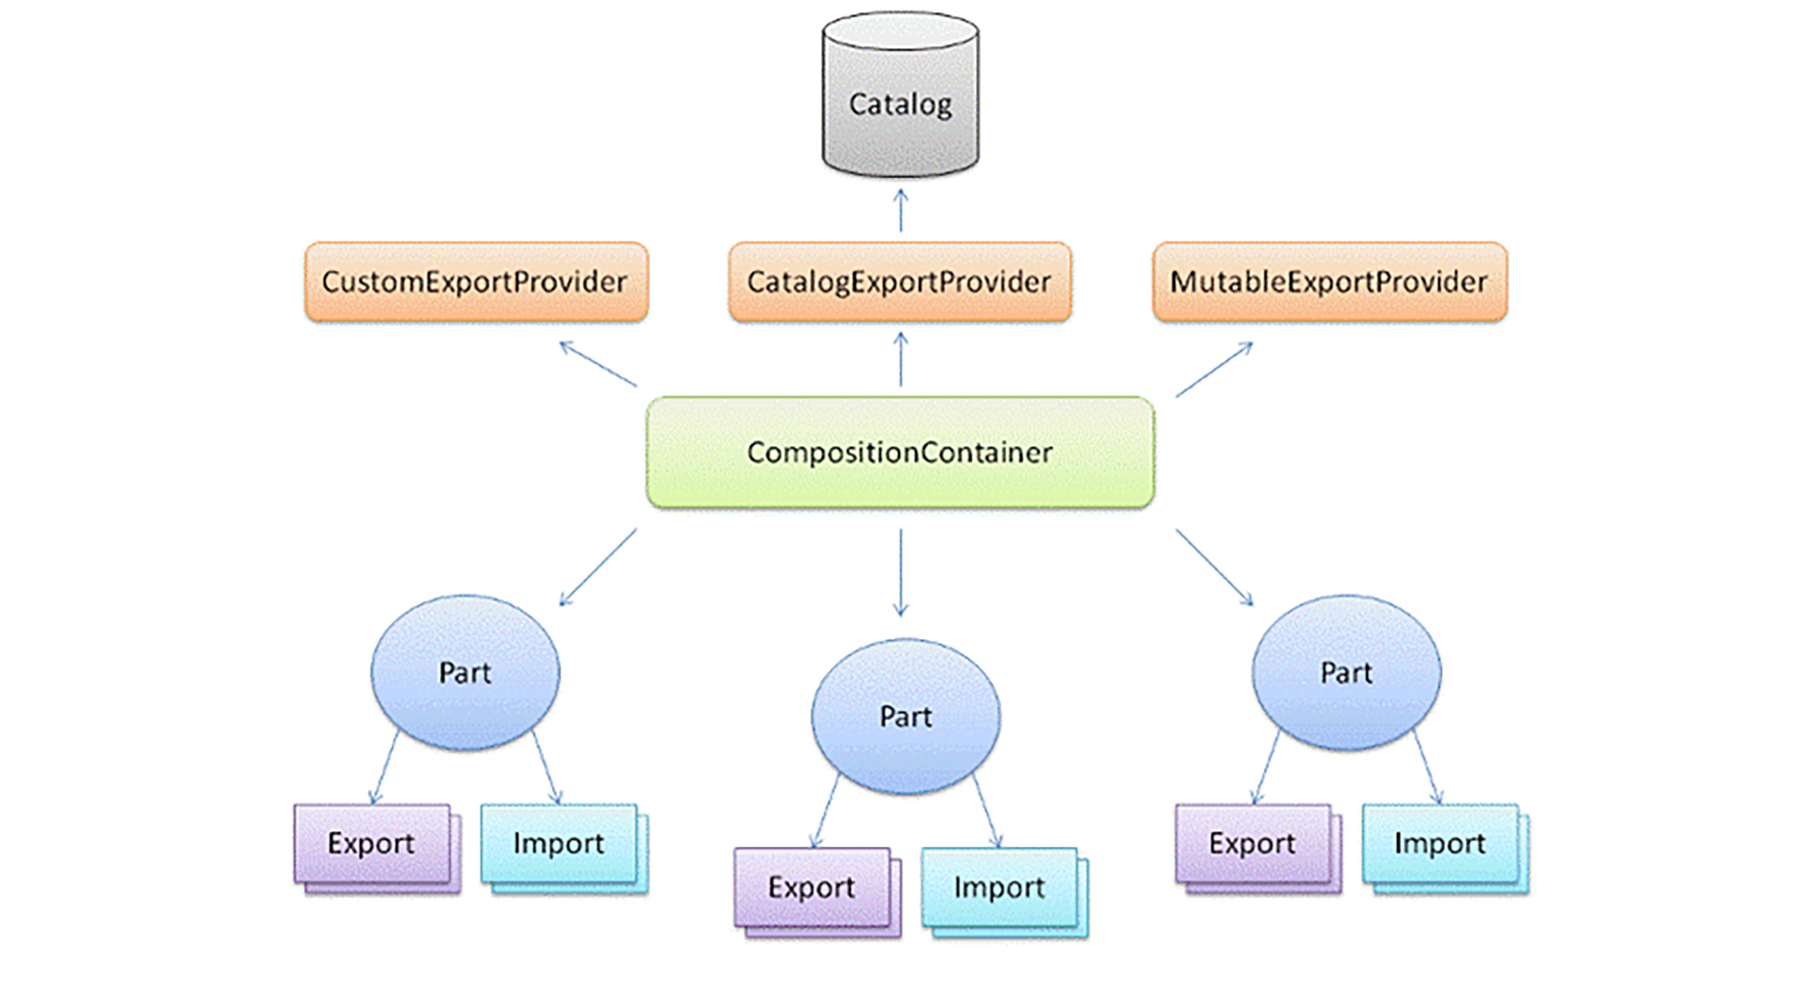
\includegraphics{images/mef_architektur.jpg}
\caption{Vereinfacht die Architektur des Managed Extensibility Framework
Quelle: msdn.microsoft.com}
\end{figure}

Die Abbilldung zeigt eine stark vereinfachte Architektur von MEF auf.
Die Hauptmodule vom MEF-Core sind Catalog und CompositionContainer. Der
Catalog kontrolliert und stellt das Laden der Komponenten sicher. Der
CompositionContainer erzeugt aus den Komponenten Instanzen und bindet
diese an die entsprechenden Variablen. Parts sind die Objekte die vom
Type Export oder Import sein können. Die Komponenten die geladen und
instanziert sind nennen sich Exports. Imports sind die Variabeln an den
Exports gebunden werden sollen.

Um das Konzept besser zu verstehen, soll der Beispielcode von Design by
Contract herangezogen werden. Die Variable proxy vom Type ISecurityStep
die die Instanz dieser Komponente enthalten soll, wäre ein „Import`` in
einer MEF Anwendung. Der SMSSecurityStep oder CookieSecurityStep wären
in einer MEF Anwendung ein Export.

MEF automatisiert die Instanzierung mit Hilfe von Catalog und Container.

\subsection{Entscheidung}\label{entscheidung-1}

MEF stellt den vollen Umfang an Funktionalität, zur Lösung der
Problematik, zu Verfügung. Der Ansatz der Umsetzung des Design by
Contract bräuchte eine geeignete Integration für die Factory. MEF bietet
des weiteren die Möglichkeit die DLL's zur Laufzeit auszutauschen und
eine automatisierte Instanzierung.

\newpage

\subsection{Sicherheitsstufen Libaray-Übersicht anhand
MEF}\label{sicherheitsstufen-libaray-uxfcbersicht-anhand-mef}

Basierend auf dem Managed Extensibility Framework wird wir der Aufbau
unstrukturiert. Neu wird nicht alles in einer Library im Webservice
gespeichert sondern mehrere Libarays erstellt. Die Libaray
SecurityStepContracts beinhaltet den Contract/Vertrag der
Sicherheitsstufen ISecurityStep. Es besteht keine Abhängigkeit zwischen
dem Authenifizierungsservice und den Sicherheitsstufen.

\begin{figure}[htbp]
\centering
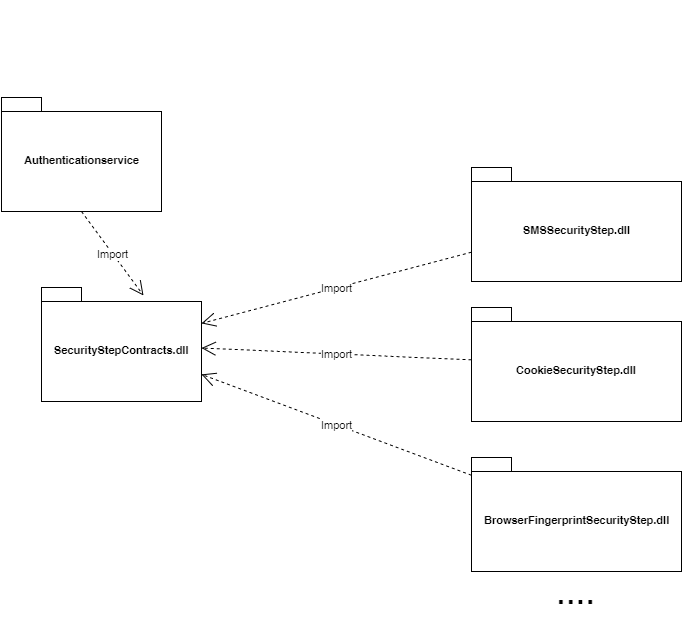
\includegraphics{images/mef_library_overview.png}
\caption{UML Library Overview}
\end{figure}

\newpage

\section{Mockup}\label{mockup}

Ein Mockup ist eine grobe Vorlage für die Design-Umsetzung. Es ist eine
ideale Möglichkeit das visuelle Konzept ab zu bilden und mit dem
Auftraggeber vorgängig anzuschauen. Die folgenden Unterkapitel bilden
die Mockups der App ab.

\subsection{Konfigurator Template}\label{konfigurator-template}

Der Konfigurator soll den Programmierer visuell beim Konfigurieren und
Verwalten seiner Authentifizierungssoftware unterstützen. Bei der
Zielgruppe handelt es sich um Programmierer. Es kann deshalb von einem
hohen Know-How ausgegangen werden. Die Oberfläche soll möglichst
effizient gestaltet sein. Die Designelemente sollen deshalb klar und
einheitlich gestaltet werden. Generell ist davon auszugehen, dass der
Programmierer beim Einrichten seines Projektes am Desktop arbeitet. Für
Auswertungen und Präsentationen kann der Programmierer durchaus auch
mobile Endgeräte verwenden. Deshalb soll die Umsetzung responsive
gestaltet werden.

\begin{figure}[htbp]
\centering
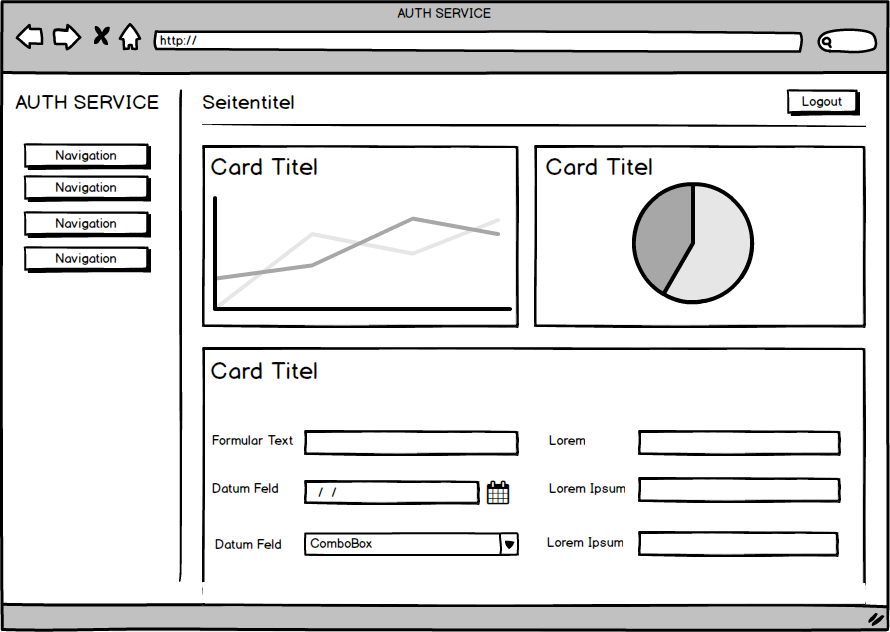
\includegraphics{images/mockups/General.png}
\caption{Mockup Konfigurator Template Desktop}
\end{figure}

\newpage

\begin{figure}[htbp]
\centering
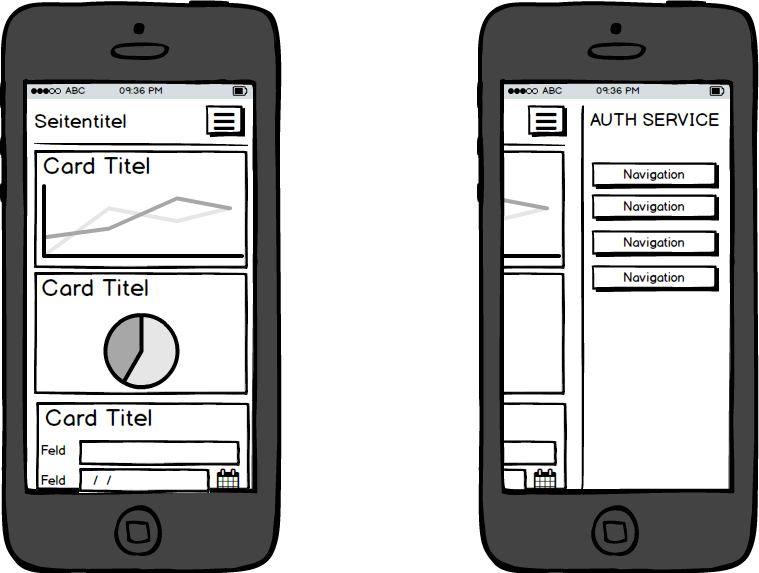
\includegraphics{images/mockups/Mobile.png}
\caption{Mockup Konfigurator Template Mobile}
\end{figure}

\subsubsection{Seitenaufbau}\label{seitenaufbau}

Im Header wird der Programmierer anhand des Seitentitels gleich über
seinen aktuellen Standort orientert.

\subsubsection{Navigation}\label{navigation}

Im Designkonzept wurde von einer Klappmenü oder Topnavigation abgesehen.
Die Wichtigkeit durch einen Klick alle Navigationspunkte zuerreichen,
überwiegte den Platzersparnissen in der Breite. Die wenigen
Navigationspunkte erlauben eine flache Navigationsstruktur. Dadurch kann
in der Desktopansicht links immer alle Navigationspunkte angezeigt
werden. Der Programmierer kann rasch auf die gewünsche Seite switchen.
In der Mobileansicht kann durch einen einzigen Klick auf die
``Burger-Navigation'' das gesamte Menü eingefahren werden. Der
Entscheid, für eine statische linke Navigationsstruktur in der
Desktopansicht, wurde ausserdem bekräftigt durch den Wunsch den
Konfigurator gestalterisch mit Farb und Bild aufzuwerten. Dies ist über
die linke Spalte einheitlich und einfach umsetzbar.

\subsubsection{Inhaltaufbau}\label{inhaltaufbau}

Trotz unterschiedlichstem Inhalt (Text, Tabellen, Diagramme, Bilder und
Formulare) und Grösse soll eine einheitliche Struktur geschaffen werden.
Die Struktur soll es erlauben einerseits Übersichten wie Dashboards mit
verschiedenen Inhalten auf einer Seite abzubilden. Die selbe Struktur
soll aber auch für Seiten mit nur einem Inhaltselement wie Registration
oder Login-Seite verwendet werden können. Verschiedene Designe lösen
diese Problematik mit einem Karten-Konzept English genannt Card Based
Design. Dabei wird jedes Inhaltselement als ``Card'' dargestellt. Die
``Card'' hat einen klar abgerenzten Darstellungsbereich. Die Card ist in
Header und Content unterteilt. Im Header wird mittels Titel (wenn auch
repetitiv) dem Anwender kommuniziert, was für ein Inhalt im Breich
Content der ``Card'' zu erwarten ist. \footnote{Weitere Informationen
  und Beispiele auf webdesigner.com \autocite{card-based-design}}

\begin{figure}[htbp]
\centering
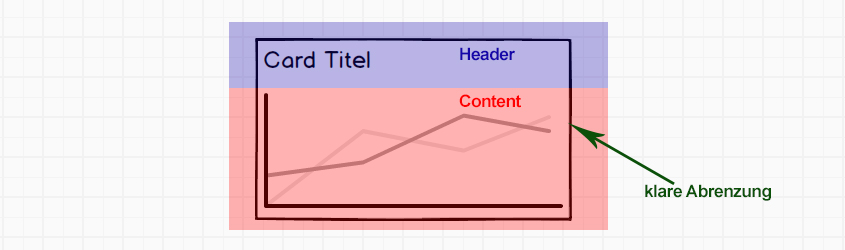
\includegraphics{images/mockups/card.jpg}
\caption{Aufbau Inhalt im Card-Design}
\end{figure}

\begin{figure}[htbp]
\centering
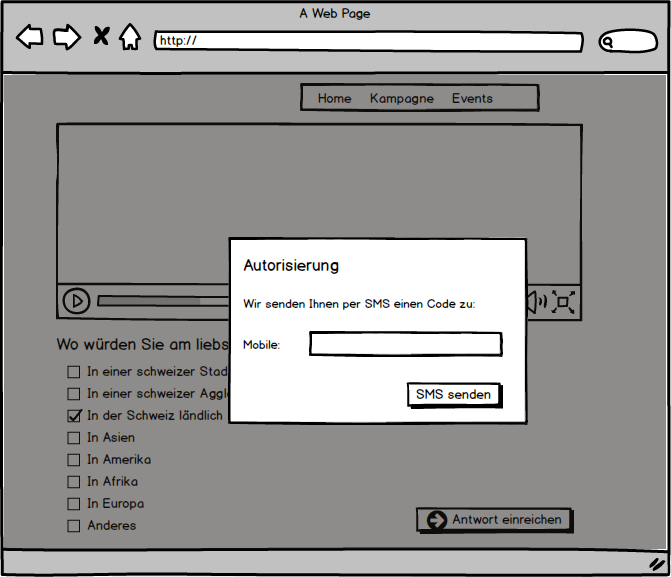
\includegraphics{images/mockups/Kundenimplementation-Desktop.png}
\caption{Aufbau Inhalt im Card-Design}
\end{figure}

\begin{figure}[htbp]
\centering
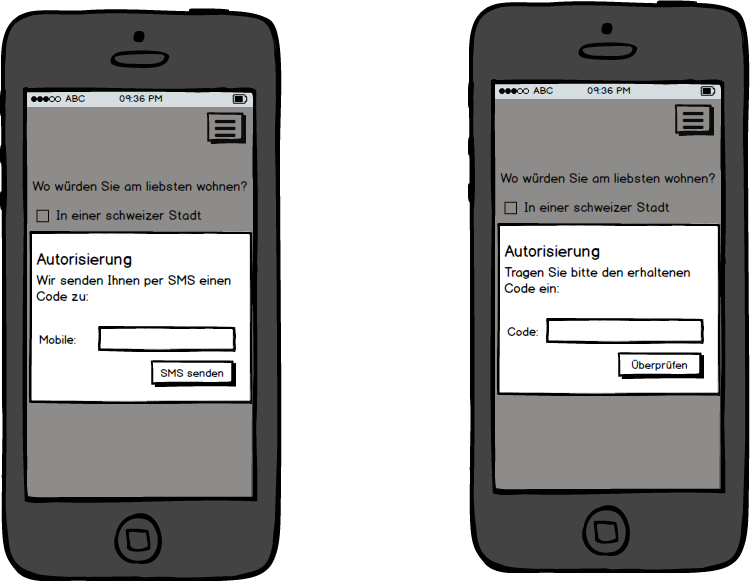
\includegraphics{images/mockups/Kundenimplementation-Mobile.png}
\caption{Aufbau Inhalt im Card-Design}
\end{figure}

\subsection{Hinweis zur Zusammenarbeit mit dem
Auftraggeber}\label{hinweis-zur-zusammenarbeit-mit-dem-auftraggeber}

Die hier abgebildeten Mockups und weitere Ansichten sind das Ergebnis
aus den Absprache mit dem Auftraggeber. Sie sind vom Auftraggeber
abgenommen und zur Impelmentation freigegeben\footnote{Alle Freigaben
  sind in der Beilage-Datei oder auf dem gihtub-Account einsehbar
  \newpage}

\section{Wahl des Applikation
Hosters}\label{wahl-des-applikation-hosters}

\subsection{Asp.net Shared Hosting}\label{asp.net-shared-hosting}

Ein Asp.net Shared Hosting ist durchaus für komplexere Webapplikationen
wie der Authentifizierungservice ausgerichtet. Die Kosten sind jährlich
fix und nicht abhängig von der eigentlichen Nutzung. Überschreitet die
Applikation den Speicherbedarf, Zugriffszahlen oder Traffic kann auf ein
grösseres Paket aktualisiert werden. Wechsel zu einem kleineren Paket
ist meist nur jährlich möglich. Die Skalierbarkeit ist stark
eingeschränkt. Die Daten können innerhalb der Schweiz gespeichert
werden. Der zuständige Systemtechniker ist meist direkt oder indirekt
kontaktierbar. Spezielle Konfigurationen am Hosting sind nicht möglich.
Die Datencenter sind meist nicht redundant geführt. Fällt das
Datencenter aus ist, die Applikation nicht verfügbar.

\subsection{Cloud Hosting}\label{cloud-hosting}

Die Serverkosten sind direkt von der eigentlichen Nutzung abhängig. Das
Hosting ist skalierbar und kann sich automatisiert an den aktuellen
Nutzungsbedürfnissen anpassen. Die realen Kosten sind im vornherein
schwerer zu definieren. Die Daten sind in der Cloud redundant geführt.
Fällt ein Datencenter aus kann ein anderes dessen Aufgabe übernehmen.
Ein Anbieter der direkt Asp.net Webservice als Hostingservice anbietet
wurde nicht gefunden.\footnote{Stand 18. Dezember 2015} Indirekt über
z.b. über ein Docker Image könnte auch ein Schweizer Anbieter
berücksichtigt werden. Die genutzten Serverdienste können komplett an
seinen eigenen Bedürfnissen angepasst werden.

\subsection{Entscheidung}\label{entscheidung-2}

Skalierbarkeit, nutzungsabhängige Kosten, Freiheit in der
Serverdienst-Konfiguration überwiegen der einfachen Speicherung der
Daten in der Schweiz. Ausserdem wird das einfache publishen
(veröffentlichen) einer Web-Application aus dem Visual Studio bei allen
Cloudanbieter angeboten (bei Shared Hosting sind es nur vereinzelte
Anbieter), was den Development Workflow erheblich unterstützt.

\section{Authentifizierungsmöglichkeiten}\label{authentifizierungsmuxf6glichkeiten}

\section{Domänenmodell}\label{domuxe4nenmodell}

\subsection{Entitäten}\label{entituxe4ten}

\section{Systemarchitektur}\label{systemarchitektur}

Gemäss den nichtfunktionalen Anforderungen muss die Serversoftware -
unter anderem - folgende Eigenschaften erfüllen:

\begin{itemize}
\tightlist
\item
  Hohe Verfügbarkeit von 99.9\%
\item
  Wartbarkeit
\item
  Performance
\end{itemize}

Die Softwarearchitektur wurde im Hinblick auf diese Anforderungen
erstellt.

\newpage

\chapter{Studie}\label{studie}

\section{Art der Studie}\label{art-der-studie}

Wie die Aufgabenstellung und der Auftraggeber fordert, wird eine Studie
in Form einer Umfrage mit Hilfe eines digitalen Fragebogens
durchgeführt. Bevor die Studie aufgebaut wird gilt es sich Vor- und
Nachteile einer schriftlichen Befragungen bewusst zu machen und
basierend auf diesem Wissen die Studie zu planen.

\subsection{Vor - und Nachteile schriftlicher
Fragebogen}\label{vor---und-nachteile-schriftlicher-fragebogen}

Schriftliche Befragungen mit Fragebogen können in verschiedenen
Varianten durchgeführt werden. Deshalb unterscheiden sich zwischen den
Varianten gewisse Vor- und Nachteile zu persönlich-mündlichen oder
telefonischen Studie. Es wird versucht, die Möglichkeiten und Grenzen
mit dem grössten gemeinsamen Nenner aufzuführen. Folgende Punkte ergeben
die wichtigsten Vorteile:

\begin{itemize}
\tightlist
\item
  Die Kosten sind geringer. Hippler \footnote{\autocite{hippler}}
  definiert den Richtwert von einem Viertel der Kosten zu einer
  persönlich-mündlichen oder telfonischen Studie.
\item
  Schriftliche Befragungen mit Fragebogen kann in einem relativ kurzen
  Zeitrum realisiert werden
\item
  Dem zu Befragenden kann eine grössere Anonymität gegeben werden
\item
  Verteilung in verschiedene Regionen einfach und zeitnah möglich.
  Insbesondere bei Online Umfrage.
\item
  Einfluss von aussen gering. Zahlreiche Studien\footnote{Studien und
    Erklärungen zu Fremdbestimmung durch François
    Höpflinger\autocite{umfragemethodik}} belegen, dass Personen welche
  eine Studie im Interview die Beantwortung beeinflussen
\item
  Die Antworten der befragten sind durch die Abwesenheit des
  Interviewers und durch die Anonymität ehrlicher. Dieser Punkt ist
  wissenschaftlich jedoch noch ziemlich umstritten. Schnell bezweifelen
  verschiedene Psychologen und Soziologen diesen Umstand. So auch
  Dr.~Reuband in seinem Paper ``Möglichkeiten und Probleme des Einsatzes
  postalischer Befragungen'' \footnote{\autocite{kzfss01}}
\end{itemize}

Diesen Vorteilen stehen auch gewisse Nachteile gegenüber. Die folgenden
Punkte erläutern die wichtigsten Nachteile die verschiedene Varianten
von Fragebögen gemeinsam haben:

\begin{itemize}
\tightlist
\item
  Wenn eine Studie eine zu grosse Nonresponse-Rate hat, ist eine
  Verallgemeinerung der Resultate unzulässig. Kurz die Bachelorarbeit
  würde mit der Studie das Ziel verfehlen. Bei einer schriftlichen
  Studie kann die Ausfallquote aber nicht im Vornherein eingeschätzt
  werden.
\item
  Die Datenerhebungssituation kann nicht kontrolliert oder bestimmt
  werden. Wo und unter welchen Umständen der Fragebogen beantwortet wird
  kann nicht bestimmt und höchstens erfragt werden.
\item
  Nachfragen basierend auf Antworten können nicht spontan gestellt
  werden, sondern müssen im Vornherein geplant werden.
\item
  Bestimmte Bevölkerungsteile werden durch diese Art der Studie
  ausgeschlossen. Zum Beispiel Analphabeten oder bei Onlineumfragen
  Personen mit zu wenig technischem Know-How oder Hardware.
\end{itemize}

\subsection{Fazit}\label{fazit}

Es gilt also die Vorteile der schriftlichen Fragebogen bei der
Gestaltung der Studie zu nutzen. Das bestimme Bevölkerungsteile
ausgeschlossen werden, verfältscht das Ergebniss nicht, da die
Anforderung für die Umfrage geringer oder gleich hoch ist wie die der
nutzung eines Social-Media Moduls. Die Nonresponse-Rate ist ein Risiko,
dass unbedingt Rechnung getragen werden muss um nicht eine ungültige
Studie zu erhalten. Damit die Problematik Nonresponse-Rate, der Umgang
mit der Datenerhubbssituation und eine geplante vorhersehbare
Fragestellung ausgefürt werdne kann gilt es sich weiter den korrekten
Aufbau einer Studie zu recherchieren.

\newpage

\section{Hauptziel der Studie}\label{hauptziel-der-studie}

In den vergangenen Kapiteln wurden immer wieder verschiedene
Authentzifizierungsarten erwähnt und beschrieben. Diese verschiedenen
Möglichkeiten gilt es mit einander zu vergleichen.

\section{Aufbau Gesamtkonzept}\label{aufbau-gesamtkonzept}

``Ein Fragebogen soll als Gesamtkomzept (Einleitung, Hauptteil, Endteil,
Design, Aufmachung) betrachtet werden, in dem die Reihenfolge und die
Struktur der Frage wichtige Einflussfaktoren zur Erlangung korrekter
Daten sind'' \footnote{Zitat vom Institut für webbasierte Kommunikation
  und E-Learning und Gräf et al. 2001 \autocite{fragebogen}}

In den folgenden Abschnitten wird die Theorie für die Entwicklung dieses
Gesamtkonzept abgebildet.

\subsection{Einleitung}\label{einleitung}

Die Einleitung soll die Befragten motivieren an der Studie teilzunehmen
und allgemeine Hinweise zur Studie geben. Die folgenden Fragen wurden
Batinic (WWW-Fragebogengenerator) und dem Institut für webbasierte
Kommunikation und E-Learning zusammen getragen und und für die Studie
der Bachelorarbeit beantwortet:

\subsubsection{Wer wird befragt?}\label{wer-wird-befragt}

Die Hauptzielgruppe sind Schweizer welche Deutsch sprechen. Die
Nebenzielgruppe sind Personen die Deutsch sprechen aus anderen Nationen.
Die Telnehmer sollen die technische Know-How besitzen an einem
Social-Media Modul teilzunehmen und den Internetzugriff haben.

\subsubsection{Was ist der Zweck bzw. das Ziel der
Untersuchung?}\label{was-ist-der-zweck-bzw.-das-ziel-der-untersuchung}

Die Studie dient dem Programmierer zur richtigen Konfiugration der
Authentifizierungsmethode für seinen aktuellen Verwendungszweck.

\subsubsection{Was passiert mit den
Ergebnissen?}\label{was-passiert-mit-den-ergebnissen}

Die Ergebnisse werden Programmierer zum Konfigurieren der
Authentifizierungsmethode zur Verfügung gestellt und in der
Bachelorarbeit veröffentlicht.

\subsubsection{Können die Ergebnisse eingesehen
werden?}\label{kuxf6nnen-die-ergebnisse-eingesehen-werden}

Durch diesen Punkt kann besonders Vertrauen und Wohlwollen gewonnen
werden \footnote{\autocite{fragebogen}}. Deshalb soll das Kapitel Studie
der Bachelorarbeit auf Wunsch den Befragten per E-Mail zugesendet
werden.

\subsubsection{Wer führt die Befragung
durch?}\label{wer-fuxfchrt-die-befragung-durch}

ZHAW Student Christian Bachmann im Auftrag der inaffect AG

\subsubsection{Kontakt für Support und
Fragen}\label{kontakt-fuxfcr-support-und-fragen}

Christian Bachmann, bachmch3@students.zhaw.ch

\subsubsection{Wie viel Zeit muss der Befragte
Investieren?}\label{wie-viel-zeit-muss-der-befragte-investieren}

Eine Einschätzung der durchschnittlich benötigen Zeit und Anzahl der
Fragen sollte genannt werden. Folgend ist das Diagramm aus der Studie
von Bosnjak und Batini abgebildet. Die Erkenntnis aus der Studie zeigt,
dass nicht nur unter dem Motto je kürzer desto besser gehandelt werden
sollte. Die Studie ist jedoch schon 15 Jahren alt und ist deshalb
differenzierter zu sehen. Die Studie der Bachelorarbeit streben einen
Aufwand von 8-12 Minuten an.

\newpage

\subsection{Hauptteil/Fragen}\label{hauptteilfragen}

Offensichtlich stellt der Hauptteil den Löwenanteil des Aufwands dar.

\subsubsection{Erste Frage}\label{erste-frage}

Die erste Frage ist nach Dillman\footnote{\autocite{dillman}} von
grosser Bedeutung. Mit ihr wird Motivation und Einsatz für den ganzen
Fragebogen gesetzt. Diese Frage soll als Interesse und Neugier der
Befragten bewirken.

Das Institut für webbasierte Kommunikation und E-Learning hat dafür aus
verschiedenen Studien die wichtigsten Kriterien für eine erfolgreiche
erste Frage zusammen getragen\footnote{\autocite{fragebogen}}: -
\textbf{Einfache Formulierung} Der Befragte versteht sofort um was es
geht und glaubt daran dass er die Fragen meistern kann - \textbf{Kurze
Beantwortungszeit, keine offenen Fragen} Ein schnelles überwinden der
ersten ``Hürde'' motiviert den Teilnehmer - \textbf{Angstabbauend}
Ängste wie z.b. die des nicht Beantworten können soll abgebaut werden. -
\textbf{Inhaltlich einführen} Die Frage soll in das Thema einführen und
im Idealfall Interesse und Neugier wecken - \textbf{Keine Fragen zur
Person oder zur Ihrem demographischen Eigenschaften}

Es kann Sinn machen eine ``perfekte'' Einstiegsfrage zu erstellen, die
in der Auswertung der Ergebnisse nicht berücksichtigt wird. Sie dient
lediglich die Anforderungen einzuhalten und en Teilnehmer einen
positives Einstiegserlebnis zu vermitteln.

Die 1. Frage der Studie dieser Bachelorarbeit: Hatten Sie schon einmal
das Gefühl, dass an einem Onlinewettbewerb gemogelt werden kann? 0 Ja 0
Nein

\subsubsection{Funktion der fragebogen}\label{funktion-der-fragebogen}

Fragen sollen eine Funktion übernehmen. Dabei schlägt Kleber\footnote{\autocite{kleber92}}
folgende Klassifizierung vor: - Übergangs- und Vorbereitungsfragen für
Themenwechsel, - Ablenkungs- und Pufferfragen zur Minderung von
Ausstrahlungseffekten, - Filterfragen zum Übergehen von eventuell
irrelevanten Fragen, - Rangier- und Konzentrationsfragen zum Auflockern
langer Darstellungen, - Motivationsfragen zur Stärkung des
Selbstvertrauens und Verminderung von Hemmungen, - Kontrollfragen als
Wahrheitskontrolle der Antworten bzw. Sichtbarmachen von Widersprüchen.

Diese Klassifizierung soll helfen den Fragebogen zu gestalten.

\subsubsection{Frageart}\label{frageart}

Bei der Stellung der Frage sollte festgestellt werden welche Art von
Frage gestellt wird. Da sich dadurch die Antwort markantlich
unterscheidet. Folgende 3 Hauptgruppen gibt es -
\textbf{Einstellungsfragen} Dieser Fragestellung bezieht sich auf
``Wunschbarkeit oder negativen bzw. Beurteilung , den Befragte mit
bestimmten Statements verbinden. - \textbf{Verhaltensfragen} Dabei wird
direkt auf das Verhalten des Befragten bezug genommen. Dabei muss
beachtet werden, dass der Befragte sein Verhalten selbst beschreibt.
Einerseits entspricht die Selbstwahrnehmung der Teilnehmer teilweise
nicht der Realität anderseits kann die Antwort auch dem Wunschdenken des
Befragten zugrunde liegen - \textbf{Eigenschftsfragen} Diese
Fragestellung fragt nach den Eigenschaften von Personen. Vielfach sind
es persönliche und demographische Daten.

\subsubsection{Fragetypen}\label{fragetypen}

Die Fragen können generell in zwei Typen unterteilt werden

\begin{longtable}[c]{@{}lc@{}}
\caption{Fragetypen}\tabularnewline
\toprule
\begin{minipage}[b]{0.24\columnwidth}\raggedright\strut
\textbf{Form}
\strut\end{minipage} &
\begin{minipage}[b]{0.70\columnwidth}\centering\strut
\textbf{Eigenschaften}
\strut\end{minipage}\tabularnewline
\midrule
\endfirsthead
\toprule
\begin{minipage}[b]{0.24\columnwidth}\raggedright\strut
\textbf{Form}
\strut\end{minipage} &
\begin{minipage}[b]{0.70\columnwidth}\centering\strut
\textbf{Eigenschaften}
\strut\end{minipage}\tabularnewline
\midrule
\endhead
\begin{minipage}[t]{0.24\columnwidth}\raggedright\strut
Offene Frage
\strut\end{minipage} &
\begin{minipage}[t]{0.70\columnwidth}\centering\strut
Der Aufwand bei der Auswertung ist sehr hoch. Ungeübte Teilnehmer können
unverwertbare Antworten niederschreiben. Antworten sind schwer
vergleichbar Dafür Teilnehmer kann sich so ausdrücken wie er möchte. Er
wird nicht durch vorgegebene Antworten beeinflusst.
\strut\end{minipage}\tabularnewline
\begin{minipage}[t]{0.24\columnwidth}\raggedright\strut
Geschlossene Frage
\strut\end{minipage} &
\begin{minipage}[t]{0.70\columnwidth}\centering\strut
Leichte Auswertung. Gefahr besteht, dass der Teilnehmer ratet und durch
die Antworten beeinflusst wird. Der Vorbereitungsaufwand für die Frage
ist hoch. Auswahlmöglichkeiten für die Antwort könnten irelevant sein.
\strut\end{minipage}\tabularnewline
\bottomrule
\end{longtable}

\subsection{Abschluss}\label{abschluss}

Der Abschluss des Fragebogens kann sehr kurz gehalten werden. Folgende
Elemente sollten enthalten sein:

\subsubsection{Dankensformel}\label{dankensformel}

Eine kurze Dankensformel gehört zum guten Ton und motiviert den
Teilnehmer die Umfrage korrekt abzuschliessen.

\subsubsection{Einladung zur
Kommentierung}\label{einladung-zur-kommentierung}

Durch Kommentare am Schluss können Befrate dem Untersucher Hinweise
zukommenlassen die für die Auswertung und weitere Untersuchungen
dienlich sind. Dieser Möglichkeit wird nach der Erfahrung von
Reuband\footnote{\autocite{kzfss01}} gewürdigt.

\section{Umsetzung Gesamtkonzept}\label{umsetzung-gesamtkonzept}

Basierend auf der Erarbeitung der Theoretischen Umsetzung eines
Gesamtkonzepts einer wissenschaftlichen Studie, gilt es nun dieses
Umzusetzen.

\chapter{ProofOfConcept}\label{proofofconcept}

\section{Techologien}\label{techologien}

Der Auftraggeber möchte dass die aktuell in seinem Betrieb eingesetzten
Technologien für die Implementation der Arbeit verwendet werden. Die
Technologien wurden abgesprochen und im folgenden Kapitel erklärt.

\subsection{C-Sharp}\label{c-sharp}

Im Rahmen der Einführung von .net veröffentlichte Microsoft 2002 die
Programmiersprache C-Sharp oder verkürzt C\#. C\# orientiert sich stark
an Java, C++, Haskell und Delphi. Daher liegt es Nahe das C\# eine
objektorientierte Programmiersprache ist und der Wechsel von den zu
vorgenannten Programmiersprachen auf C\# einfach fällt.

Neben Grundprinzipen der objektorientierten Programmierung resultiert
aus folgende innovativen Sprach-Konstrukte eine vereinfachte
Programmierung:

\begin{itemize}
\tightlist
\item
  Gekapselte Methodensignaturen, Delegaten genannt, die typsichere
  Ereignisbenachrichtigungen ermöglichen
\item
  Eigenschaften, die als Accessoren für private Membervariablen dienen
\item
  Attribute, die zur Laufzeit deklarative Metadaten zu Typen
  bereitstellen
\item
  Inline-XML-Dokumentationskommentare
\item
  Sprachintegrierte Abfrage (Language-Integrated Query, LINQ), die
  integrierte Abfragefunktionen für eine Vielzahl von Datenquellen
  bereitstellt
\end{itemize}

Der C\#-Erstellungsprozess ist im Vergleich zu C und C++ einfach und
flexibler als in Java. Es gibt keine separaten Headerdateien und es ist
nicht erforderlich, Methoden und Typen in einer bestimmten Reihenfolge
zu deklarieren. Eine C\#-Quelldatei kann eine beliebige Anzahl von
Klassen, Strukturen, Schnittstellen und Ereignissen definieren.
\footnote{Quelle:\autocite{csharpbasic}}

\subsection{ASP.net Web API 2 / ASP.net MVC
Framework}\label{asp.net-web-api-2-asp.net-mvc-framework}

Microsoft entwickelte mit dem ASP.net MVC Framework ein schlankes und
einfach zu testendes Präsentationsframework. Wie im Namen enthalten
basiert das Framework auf dem MVC-Pattern. Die klare Trennung von
Eingabelogik, Geschftslogik und Präsentationslogik wird durch die vom
Framework bereitgestellten Komponenten unterstützt. Um
RESTful-Webservices einfach entwickeln zu können stellt Microsoft mit
ASP.net Web API 2 eine einfache zu verwendendes und starkes Software
Paket zur Verfügung. ASP.net Web API 2 basiert auf dem ASP.net MVC
Framework. \footnote{Quelle:\autocite{csharpbasic}}

\newpage

\subsection{Entity Framework}\label{entity-framework}

Entity Framework (EF) ist eine objektrelationale Zuordnung, die
.NET-Entwicklern über domänenspezifische Objekte die Nutzung
relationaler Daten ermöglicht. Ein Grossteil des Datenzugriffscodes, den
Entwickler normalerweise programmieren, muss folglich nicht geschrieben
werden. {[}\^{}efbasic{]}

\subsection{AngularJS}\label{angularjs}

Mittels AngularJS wird die Client-Browser App entwickelt. AngularJS ist
ein Javascript Framework, welches OpenSource von Google Inc.
veröffentlicht wurde. AngularJS macht einen Grossteil des Codes, den man
normalerweise schreibt, überflüssig. Die Reduktion des Codes begründet
sich durch die Automatisierung von Standardaufgaben. Die manuelle
DOM-Selektion, DOM-Manipulation und Event-Behandlung werden durch
AngularJS überflüssig. Durch Einsatz von Direktiven und Modulen wird die
Wiederverwendbarkeit von Code ermöglicht.

Die normalen Datentypen von JavaScript können verwendet werden. Dadurch
ist es sehr einfach möglich, fremde Bibliotheken einzubinden, ohne eine
weitere Zwischenschicht (Glue Code) zu implementieren. Die Methode, die
AngularJS dazu verwendet nennt sich Dirty-Checking und wird im
Vertiefungskapitel näher erklärt.{[}\^{}angularjsbasic{]}

\subsection{JSON}\label{json}

Zwischen der AngularJS WebApp und dem Webservice dient JSON(JavaScript
Object Notation) als Datenübertragungsformat. JSON zeichnet sich durch
seine schlanke Notation und der objektnahen Darstellung aus
{[}\^{}efbasic{]}: Quelle \autocite{efbasic} {[}\^{}angularjsbasic{]}:
Quelle \autocite{angularjsbasic}

\chapter{Fazit}\label{fazit-1}

\newpage

\appendix

\hypertarget{glossar}{\chapter{Glossar}\label{glossar}}

\textbf{2FA} 2FA bedeutet Zwei-Faktor-Authentifizierung. Weitere Infos
im Kapitel Authentifizierungs Kompononten

\textbf{Github} Github ist ein Cloud basierter SourceCode
Verwaltungsdienst für Git. \url{https://github.com}

\textbf{Non-Response} Nichtbeantwortung einer oder mehrerer einzelner
Fragen. Die Repräsentativität einer Befragung hängt stark ab von der
Rücklaufquote, auch Response-Rate genannt.

\textbf{ORM} ORM steht für object-relational mapping und ist eine
Technik mit der Objekte einer Anwendung in einem relationalen
Datenbanksystem abgelegt werden kann.\\

\textbf{REST / Restfull} REST steht für Representational State Transfer.
REST ist eine Software Architektur des Webs. System welche die REST
Architektur einhalten nennt man RESTful. REST System kommunizieren
allgemein über das HTTP-Protokoll und nutzen die gleichen HTTP verbs wie
ein Browser der eine Webseite abfragt. Neben GET und POST werden die
weniger bekannten Verben PUT und Delete verwendet. Die URI beschreibt
die zu beziehende oder verändernde Webressource.

\chapter{Verzeichnisse}\label{verzeichnisse}

Neues Verzeichnisse

\section{Abbildungsverzeichnis}\label{abbildungsverzeichnis}

\renewcommand{\listfigurename}{} 

\begingroup\let\clearpage\relax
\listoffigures
\endgroup

\pagebreak

\section{Quellenverzeichnis}\label{quellenverzeichnis}

\renewcommand{\bibname}{}

\begingroup \let\clearpage\relax
\printbibliography
\endgroup

\pagebreak

\section{Tabellenverzeichnis}\label{tabellenverzeichnis}

\renewcommand{\listtablename}{} 

\begingroup \let\clearpage\relax
\listoftables
\endgroup





\end{document}